\documentclass[11pt,a4paper,twoside,openright]{book}

%\usepackage{hyperref}
\usepackage[dvips]{graphicx}
\usepackage{tabularx}
\usepackage{url}
\usepackage{subfigure}
\usepackage{afterpage}
\usepackage{amsmath,amssymb}            
\usepackage{rotating}  
\usepackage{fancyhdr}  
\usepackage[scriptsize]{caption} 
\usepackage{glossaries}
\makeglossaries
\hyphenation{a-gen-tiz-za-zio-ne}

\setlength{\paperwidth}{16cm}
\setlength{\paperheight}{24cm}
\setlength{\oddsidemargin} {2. cm}
\setlength{\evensidemargin} {2. cm}
\addtolength{\oddsidemargin} {-0.4 cm}
\addtolength{\evensidemargin} {-0.4 cm}

\usepackage[italian]{babel}
\usepackage[latin1]{inputenc}
\renewcommand{\captionfont}{\normalfont \sffamily \itshape \small}
\newcommand{\argmax}{\operatornamewithlimits{argmax}}
\pagestyle{empty}
\graphicspath{./pictures}

% Voci del glossario
\newglossaryentry{scena}{name={scena},description={luogo di interesse per una particolare applicazione di monitoraggio video}}

\newglossaryentry{inquadratura}{name={inquadratura},description={porzione dello spazio fisico che viene acquisito dal sensore della camera}}

\newglossaryentry{frame}{name={frame},description={immagine acquisita dal sensore della camera}}

\newglossaryentry{framerate}{name={framerate},description={frequenza di acquisizione dei frame da parte della camera}}

\newglossaryentry{tampering}{name={tampering},description={letteralmente \textit{manomissione}, nel contesto della tesi indica un qualsiasi evento che non permette una corretta ripresa della scena da parte della camera}}

\begin{document}
\thispagestyle{empty}
%\begin{titlepage}
\vspace*{-1.5cm} \bfseries{
\begin{center}
  \large
  POLITECNICO DI MILANO\\
  \normalsize
  Corso di Laurea Magistrale in Ingegneria Informatica\\
  Dipartimento di Elettronica, Informazione e Bioingegneria\\
  \begin{figure}[htbp]
    \begin{center}
      \includegraphics[width=3.5cm]{./pictures/logopm}
%	\psfig{file=./pictures/logopm.jpg,width=3.5cm}
    \end{center}
  \end{figure}
  \vspace*{0.3cm} \LARGE



  \textbf{ALGORITMO DI TAMPERING DETECTION OTTIMIZZATO TRAMITE SEGMENTAZIONE DELLA SCENA INQUADRATA}\\



%  \vspace*{.75truecm} \large
%  AI \& R Lab \\
%  Laboratorio di Intelligenza Artificiale \\
%  e Robotica del Politecnico di Milano
\end{center}
\vspace*{3.0cm} \large
\begin{flushleft}


	Relatore: Prof. Giacomo BORACCHI \\
	Correlatore: Ing. Claudio MARCHISIO\\

  

\end{flushleft}
\vspace*{1.0cm}
\begin{flushright}


  Tesi di Laurea di:\\ Adriano GAIBOTTI, matricola 780200 \\ 
		       


\end{flushright}
\vspace*{0.5cm}
\begin{center}



  Anno Accademico 2013-2014
\end{center} \clearpage
}

\frontmatter
\thispagestyle{empty} \normalfont \cleardoublepage
\vspace{17cm}

%\large
\begin{flushright}
\itshape{ A Gigino }
\end{flushright}

\thispagestyle{empty}  \cleardoublepage
\newpage
\chapter*{Sommario}

\addcontentsline{toc}{chapter}{Sommario}

Nel campo dei sistemi di monitoraggio video, uno dei principali problemi \`e quello di identificare eventi che possano compromettere la corretta ripresa della scena.
Pu\`o capitare, ad esempio, che dell'acqua piovana si depositi sulla lente della camera, rendendo l'immagine acquisita sfocata, oppure che la camera si sposti, a causa di un intenzionale intervento umano o per eventi naturali quali una raffica di vento, e non riprenda pi\`u la scena da sorvegliare.\\
Il problema di individuare, in maniera automatica, questo tipo di eventi prende il nome di \textit{tampering detection}. 
Nella letteratura scientifica questo problema \`e stato affrontato solamente per applicazioni di \textit{videosorveglianza}, dove la camera opera con acquisizione continua, dispone di una certa potenza computazionale e viene alimentata a corrente.
Lo scopo della tesi \`e lo sviluppo di un algoritmo di tampering detection per camere intelligenti (\textit{smart camera}) e a basso consumo, da utilizzarsi in scenari di monitoraggio. In particolare, l'algoritmo \`e caratterizzato da un basso carico computazionale ed \`e pensato per scenari, tipo il monitoraggio ambientale, dove il sistema, per ridurre il consumo energetico, acquisisce e analizza poche immagini al minuto o all'ora (\textit{framerate bassi}).
In questi casi scene ad \textit{alta dinamicit\`a}, come una strada in cui passano macchine e pedoni, non permettono di identificare eventi di tampering tramite un confronto tra frame consecutivi. 
Inoltre, operando a bassi framerate, si verificano sostanziali variazioni di luminosit\`a tra immagini consecutive. \\ 
L'algoritmo proposto si basa su indicatori, estratti dalle singole immagini, calcolati a bassa complessit\`a computazionale; tali indicatori vengono monitorati nel tempo attraverso tecniche \textit{sequenziali} e \textit{one-shot} per identificare l'istante in cui avviene l'evento di tampering.
Data l'alta variabilit\`a degli indicatori utilizzati, abbiamo introdotto una fase di \textit{segmentazione} della scena, in modo da limitare l'analisi ad alcune regioni specifiche:
questo permette di migliorare le prestazioni dell'algoritmo e diminuire il numero di falsi allarmi.\\
La tesi \`e stata svolta durante un lavoro di stage presso il gruppo \textit{Advanced System Technology} di \textit{STMicroelectronics}, dove la ricerca \`e volta allo sviluppo di algoritmi intelligenti di elaborazione immagini da integrare nei propri dispositivi embedded.
Sono stati messi a punto diversi sistemi di acquisizione operanti a diversi framerate, che hanno permesso di generare i dataset per testare l'efficacia della soluzione proposta e, in particolare, dei vantaggi nell'utilizzo della segmentazione a supporto del tampering detection. 

\thispagestyle{empty} \vspace*{.75truecm} \cleardoublepage
\chapter*{Ringraziamenti}

\addcontentsline{toc}{chapter}{Ringraziamenti}

Ringrazio ................

\tableofcontents
\listoffigures
\listoftables
%\printglossaries

\mainmatter
\thispagestyle{empty} \vspace*{.75truecm} \normalfont \cleardoublepage
\pagestyle{plain}\renewcommand{\chaptermark}[1]{\markboth{\chaptername\ \thechapter.\ #1}{}} 
\renewcommand{\sectionmark}[1]{\markright{\thesection.\ #1}}         
\fancyhead[LE,RO]{\bfseries\thepage}    
                                        
\fancyhead[RE]{\bfseries\leftmark}    
\fancyhead[LO]{\bfseries\rightmark}     
\renewcommand{\headrulewidth}{0.3pt} 


\chapter{Introduzione}
\label{Introduzione}
\thispagestyle{empty}

\begin{quotation}
	{\footnotesize
		\noindent\emph{``Terence: Mi fai un gelato anche a me? Lo vorrei di pistacchio. \\
			Bud: Non ce l'ho il pistacchio. C'ho la vaniglia, cioccolato, fragola, limone e caff\`e. \\
			Terence: Ah bene. Allora fammi un cono di vaniglia e di pistacchio. \\
			Bud: No, non ce l'ho il pistacchio. C'ho la vaniglia, cioccolato, fragola, limone e caff\`e. \\
			Terence: Ah, va bene. Allora vediamo un po', fammelo al cioccolato, tutto coperto di pistacchio. \\
			Bud: Ehi, macch\'e sei sordo? Ti ho detto che il pistacchio non ce l'ho! \\
			Terence: Ok ok, non c'\`e bisogno che t'arrabbi, no? Insomma, di che ce l'hai? \\
			Bud: Ce l'ho di vaniglia, cioccolato, fragola, limone e caff\`e! \\
			Terence: Ah, ho capito. Allora fammene uno misto: mettici la fragola, il cioccolato, la vaniglia, il limone e il caff\`e. Charlie, mi raccomando il pistacchio, eh.''}
		\begin{flushright}
			Pari e dispari
		\end{flushright}
	}
\end{quotation}
\vspace{0.5cm}
Punti da sviluppare:

\section{Aumento nell'interesse dei contenuti multimediali, tra cui il \textit{monitoraggio video} (IoT, domotica,...)}
\section{Esempi videosorveglianza e webcam meteo}
\section{Problema dell'affidabilit\`a del contenuto video}
\begin{itemize}
	\item Vitale nel caso della videosorveglianza
	\item Caso webcam limitare traffico in rete evitando di inviare frame compromessi
	\item Qualit\`a del servizio
\end{itemize}
\section{Tampering Detection}
\section{Riassunto soa}
Enfatizzare il fatto che il lavoro presente in letteratura \`e legato solamente ad applicazioni di videosorveglianza
\section{Scopo della tesi}
\section{Soluzione proposta}
\section{Esperimenti fatti}
\section{Problemi rimasti aperti}
\section{Struttura della tesi}
La tesi \`e strutturata nel seguente modo.\\
Nel capitolo \ref{StatoArte} si mostra lo stato dell'arte.\\
Nel capitolo \ref{FormulazioneProblema} si illustra come \`e stato formalizzato il problema.\\
Nel capitolo \ref{SoluzioneProposta} si illustra la soluzione proposta per risolvere il problema.\\
Nel capitolo \ref{ProveSperimentali} si mostrano le prove realizzate per validare la soluzione proposta, descrivendo anche la realizzazione dei dataset e i risultati ottenuti.\\
Nel capitolo \ref{Conclusioni} si mostrano le prospettive future di ricerca e si tirano le conclusioni.
	

\chapter{Stato dell'arte}
\label{StatoArte}
\thispagestyle{empty}

%\begin{quotation}
%{\footnotesize
%\noindent{\emph{``Terence: Rotta a nord con circospezione \\
%Bud: Ehi, gli ordini li do io qui!\\
%Terence: Ok, comante\\
%Bud: Rotta a nord\\
%Terence: Soltanto?\\
%Bud: Con circospezione!''}
%}
%\begin{flushright}
%Chi Trova un Amico Trova un Tesoro
%\end{flushright}
%}
%\end{quotation}
%\vspace{0.5cm}

\noindent In questo capitolo presentiamo i concetti fondamentali della teoria alla base della \textit{visione artificiale} e dell'elaborazione di segnali e lo studio fatto finora sul problema del \textit{tampering detection}.\\
Nei Paragrafi \ref{modelloCamera} e \ref{rappresentazImmagini} diamo una visione generale del modello della camera e di come vengono rappresentate le immagini digitali, in modo da comprendere meglio gli argomenti trattati nei capitoli successivi.\\
Nel Paragrafo \ref{cdt} illustriamo le tecniche maggiormente utilizzate per identificare cambiamenti nella stazionariet\`a di un segnale o una sequenza di dati.\\
Nel Paragrafo \ref{tamperingSOA} descriviamo le soluzioni al problema del tampering detection presenti nella letteratura scientifica, definendo inoltre i concetti e la terminologia che verr\`a utilizzata nel resto della trattazione.
\section{Modello della camera}
\label{modelloCamera}
Affinch\'e un sistema di visione artificiale possa risolvere il problema per cui \`e stato progettato, \`e necessario che esso sia in grado di acquisire una porzione della realt\`a che lo circonda.
Questo compito viene svolto da un particolare sensore chiamato \textit{camera}, il cui scopo principale \`e quello di creare una \textit{proiezione} dell'ambiente \textit{tridimensionale} in un sistema \textit{bidimensionale}.
Il principio alla base della camera \`e un concetto inventato da \textit{Filippo Brunelleschi} nel XV secolo, chiamato \textit{prospettiva a punto unico di fuga} (\textit{pinhole perspective}) \cite{manetti1976vita}.
Il modello matematico utilizzato considera uno spazio tridimensionale, detto \textit{ambiente}, e un piano bidimensionale chiamato \textit{immagine}. 
I punti su tale piano sono la \textit{proiezione} dell'ambiente tridimensionale.
La proiezione \`e dovuta a un punto, chiamato \textit{centro ottico}, in cui viene convogliata la luce emanata dall'ambiente tridimensionale.
In questa astrazione, ciascun punto dello spazio tridimensionale viene associato univocamente a un punto nel piano immagine attraverso il raggio di luce che passa dal centro ottico.
\begin{figure}[tb]
	\centering
	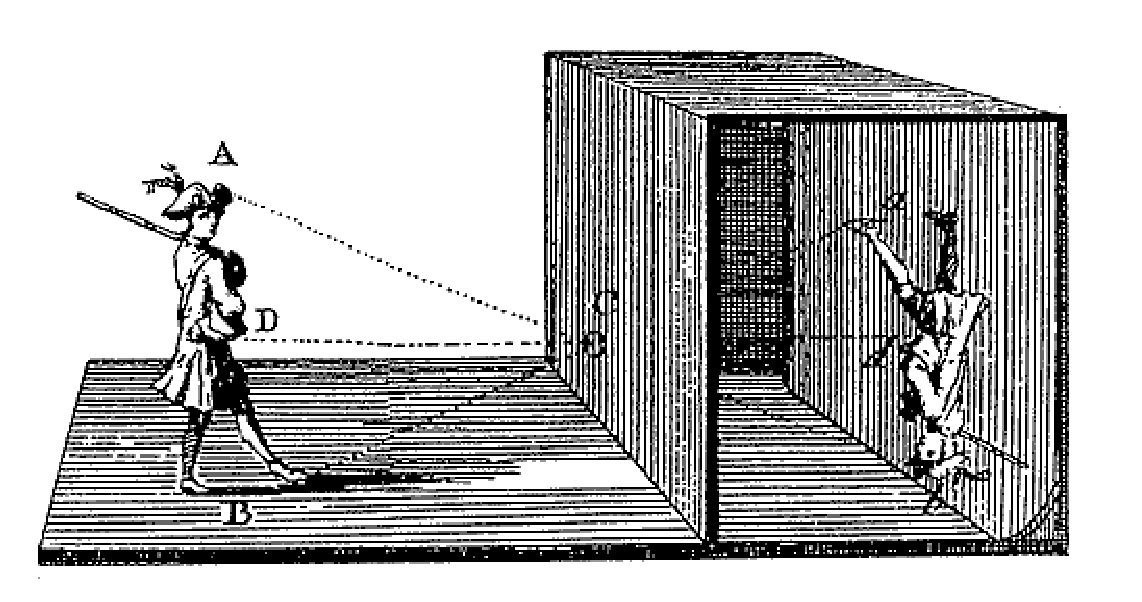
\includegraphics[width=12cm]{./pictures/cameraObscura}
	\caption[Athanasius Kircher, Principio della prospettiva nella camera obscura, 1671]{Athanasius Kircher, Principio della prospettiva nella camera obscura, 1671}
	\label{fig:prospettiva}
\end{figure} 
All'epoca di Brunelleschi, il modello del centro ottico veniva realizzato da una \textit{camera oscura}, come si pu\`o osservare nell'illustrazione in Figura \ref{fig:prospettiva}, mentre nei moderni sistemi di acquisizione viene realizzato tramite \textit{lenti ottiche}. 
\subsection{La matrice prospettica della camera}
\begin{figure}[tb]
	\centering
	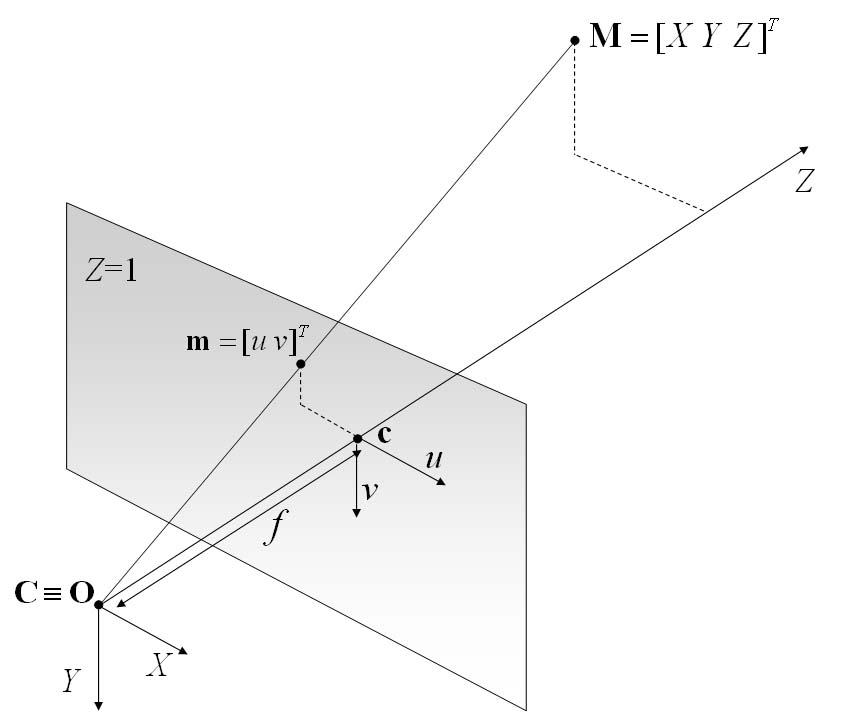
\includegraphics[width=10cm]{./pictures/modelloCamera}
	\caption{Schematizzazione del sistema ottico della camera}
	\label{fig:modelloCamera}
\end{figure} 
Nella Figura \ref{fig:modelloCamera} sono illustrati i concetti che sono utilizzati per descrivere il sistema ottico della camera.
Indichiamo con la lettera maiuscola $\textbf{M}=[X, Y, Z]^\textit{T}$ un qualsiasi punto nello spazio tridimensionale e con la lettera minuscola $\textbf{m} = [u, v]^\textit{T}$ la sua proiezione sul piano immagine dovuta al centro ottico $\textbf{C}$.
La linea che congiunge il centro ottico $\textbf{C}$ perpendicolarmente al piano immagine \`e detta \textit{asse principale}, indicata con $Z$, e il suo punto di intersezione con il piano stesso viene definita \textit{punto principale} $\textbf{c}$.
La distanza tra il punto principale e il centro ottico viene definita \textit{distanza focale},  e viene indicata con $f$.\\
La rappresentazione dei punti viene fatto attraverso le loro \textit{coordinate omogenee}.
In questo modo \`e possibile rappresentare le trasformazioni tra sistemi di coordinate di ordine differente tramite una singola trasformazione matriciale.
Chiamiamo coordinate omogenee di un punto $\textbf{m} = [u,v]$ del piano una qualsiasi terna ordinata $[U,V,W]$ di numeri reali tali che
\[W\neq 0,
\frac{U}{W}=u,
\frac{V}{W}=v.\]
Analogamente, le coordinate omogenee di un punto $\textbf{M}=[x,y,z]$ nello spazio tridimensionale saranno costituite da una quaterna di numeri $[X,Y,Z,W]$ tali che 
\[W\neq 0,
\frac{X}{W}=x,
\frac{Y}{W}=y,
\frac{Z}{W}=z.\]
La coordinata $W$ viene definita \textit{valore di scala}; nel caso $W=1$ le rimanenti coordinate omogenee rappresentano le \textit{coordinate cartesiane} del punto.\\
Consideriamo un punto $\textbf{M}$ nello spazio tridimensionale, rappresentato tramite le coordinate omogenee $[X,Y,Z,1]^\textit{T}$, e il suo punto immagine $\textbf{m}$ rappresentato dalle coordinate omogenee $[u,v,1]^\textit{T}$.
La proiezione della camera pu\`o essere espressa come
\begin{equation}
\label{eq:proiezione}
\textbf{m}=P\textbf{M},
\end{equation}
dove $P$ \`e una matrice di dimensioni $3 \times 4$ chiamata \textit{matrice prospettica} \cite{hartley2003multiple}.
Tale matrice contiene al suo interno informazioni sui parametri della camera a cui \`e associata, e descrive sia la proiezione sul piano immagine che le trasformazioni di camera rispetto al sistema di riferimento tridimensionale.
Formalmente la matrice prospettica viene definita attraverso la concatenazione di due matrici: una che rappresenta i \textit{parametri intrinseci} e un'altra che rappresenta i \textit{parametri estrinseci} \cite{forsyth2002computer}.
\begin{itemize}
	\item I \textit{parametri intrinseci} rappresentano le caratteristiche interne della camera come la distanza focale, il centro focale e le caratteristiche di \textit{distorsione} della lente.
	\item I \textit{parametri estrinseci} rappresentano la posizione della camera rispetto al sistema di riferimento dello spazio tridimensionale.
\end{itemize} 
\subsection{Parametri intrinseci}
\label{intrinsicParam}
La relazione fra le coordinate tridimensionali di un punto $\textbf{M}=[X,Y,Z]$ e le coordinate della sua proiezione $\textbf{m}=[u,v]$ \`e:
\[u=f\cdot \frac{X}{Z},\]
\[v=f\cdot \frac{Y}{Z}.\]
\begin{figure}[tb]
	\centering
	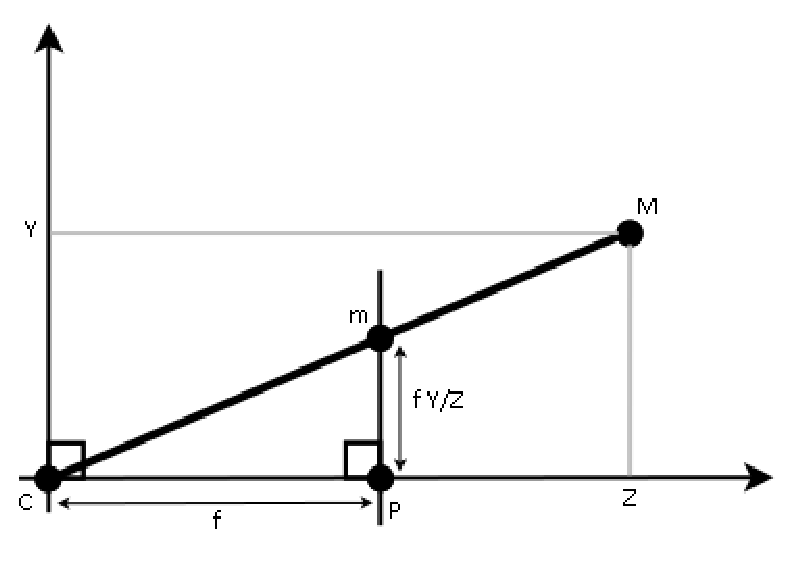
\includegraphics[width=10cm]{./pictures/mappatura2d3d}
	\caption{Similitudini tra triangoli usate nel calcolo dei parametri intrinseci}
	\label{fig:mapping}
\end{figure}
\noindent Tale relazione deriva dalle propriet\`a dei triangoli simili, come mostra la Figura \ref{fig:mapping}.
La \textit{mappatura} viene definita, dunque, dalla seguente relazione:
\begin{equation}
\label{eq:mapping}
[X,Y,Z]^\textit{T} \mapsto \left[f\cdot \frac{X}{Z}, f\cdot \frac{Y}{Z}\right]^\textit{T}.
\end{equation} 
Se il punto nello spazio e la sua proiezione sono rappresentati attraverso le loro coordinate omogenee, la \eqref{eq:mapping} pu\`o essere riscritta come
\begin{equation}
\label{eq:mappingMatrix}
\left[\begin{array}{c}
X \\ Y \\ Z \\ 1
\end{array}\right] \mapsto 
\left[\begin{array}{c}
f \cdot X \\ f \cdot Y \\ Z
\end{array}\right] = 
K \left[\begin{array}{rcl}
I & | & 0
\end{array}\right]
\left[\begin{array}{c}
X \\ Y \\ Z \\ 1
\end{array}\right],
\end{equation}
dove la matrice
\begin{equation}
\label{eq:kSimple}
K = 
\left[\begin{array}{rccl}
f & & \\
& f & \\
& & 1 
\end{array}\right]
\end{equation}
viene detta \textit{matrice di calibrazione} della camera.\\
Nella \eqref{eq:mapping} abbiamo assunto che l'origine delle coordinate del piano immagine si trovi nel punto principale, come \`e illustrato nella Figura \ref{fig:modelloCamera}.
Se consideriamo il punto principale di coordinate $[p_u, p_v]$, la \eqref{eq:mapping} diventa
 \begin{equation}
 \label{eq:mappingGeneral}
 [X,Y,Z]^\textit{T} \mapsto \left[f\cdot \frac{X}{Z}+p_u, f\cdot \frac{Y}{Z}+p_v\right]^\textit{T},
 \end{equation}
 mentre la matrice di calibrazione \eqref{eq:kSimple} diventa 
 \begin{equation}
 \label{eq:kGeneral}
 K =
  \left[\begin{array}{rcl}
  f & & p_u \\
  & f & p_v \\
  & & 1 
  \end{array}\right].
 \end{equation}
 Nel caso in cui il sensore della camera sia \textit{digitale}, l'immagine deve essere quantizzata come una matrice di $W$ colonne e $H$ righe, in cui ciascun elemento prende il nome di \textit{pixel} (dalla contrazione di \textit{picture element}).
 \begin{figure}[tb]
 	\centering
 	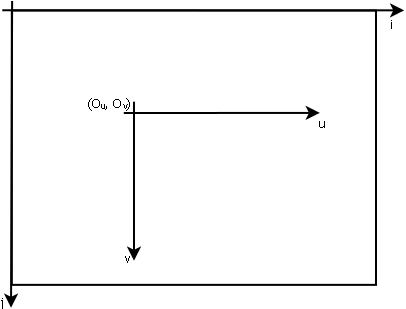
\includegraphics[width=8cm]{./pictures/griglia}
 	\caption{Coordinate di un frame}
 	\label{fig:griglia}
 \end{figure}
 Ogni pixel possiede, quindi, delle coordinate che definiscono la sua posizione sulla matrice del frame.
 Se definiamo con $(i,j)$ le coordinate del generico pixel sulla matrice del frame, dove l'origine \`e posta nell'angolo in alto a sinistra, e con $(O_u, O_v)$ le coordinate del punto principale secondo il sistema di riferimento del frame (si veda a riguardo la Figura \ref{fig:griglia}), possiamo mettere in relazione le coordinate dell'immagine con le coordinate frame nel seguente modo:
 \[ u = (i - O_u) \cdot S_u \]
 e
 \[ v = (j - O_v) \cdot S_v, \]
 dove $S_u$ e $S_v$ sono le dimensioni orizzontali e verticali del singolo pixel.
 \`E necessario introdurre, nella matrice di calibrazione, l'informazione del numero di pixel per unit\`a di distanza in coordinate immagine $m_u$ e $m_v$, rispettivamente nelle direzioni $u$ e $v$, modificando la matrice di calibrazione definita in \eqref{eq:kGeneral} come
 \begin{equation}
 \label{eq:kDigital}
 K =
 \left[\begin{array}{rccl}
 \alpha_u & & u_0\\
 & \alpha_v & v_0\\
 & & 1
 \end{array}\right],
 \end{equation}
 dove $\alpha_u = fm_u$ e $\alpha_v=fm_v$, mentre il punto principale $[p_u, p_v]$ viene riscritto come $[u_0, v_0] = [m_u p_u, m_v p_v]$. \\
 Nel caso in cui la matrice di calibrazione sia nota, la camera viene detta \textit{completamente calibrata}.\\
 La matrice di calibrazione $K$ rappresenta, quindi, il cambio di sistema di riferimento nel piano immagine, ridefinendo il centro della camera $(u_0, v_0)$ in modo che coincida con il punto principale.
 \subsection{Parametri estrinseci}
 La matrice $K$ descritta da \eqref{eq:kDigital} \`e valida per camere poste all'origine del sistema di riferimento.
Se consideriamo delle camere poste in un punto arbitrario dell'ambiente, quindi, \`e necessario che le coordinate dei punti, definite nel sistema di riferimento tridimensionale, siano ridefinite secondo il sistema di coordinate della camera.
 \begin{figure}[tb]
 	\centering
 	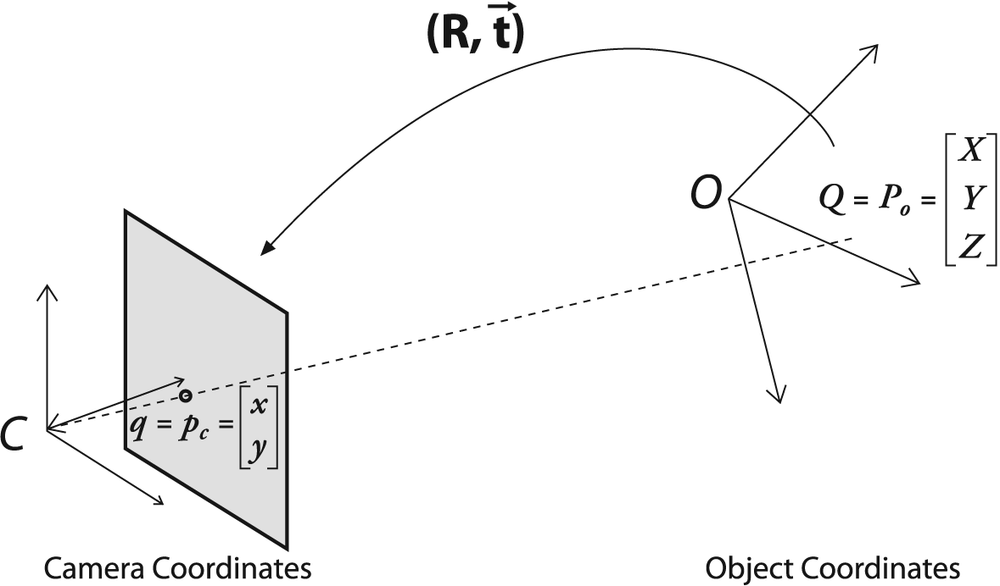
\includegraphics[width=8cm]{./pictures/rt}
 	\caption{Trasformazione dal sistema di coordinate dell'ambiente a quello della camera}
 	\label{fig:rt}
 \end{figure}
Questa trasformazione viene definita attraverso una \textit{rototraslazione}, nello spazio, del sistema di riferimento dell'ambiente, in modo che coincida con quello della camera.
Se $\tilde{\textbf{M}}$ rappresenta le coordinate cartesiane di un punto nel sistema di riferimento dell'ambiente e $\tilde{\textbf{M}}_{cam}$ rappresenta lo stesso punto nel sistema di riferimento della camera, si pu\`o scrivere
\begin{equation}
\label{eq:rototrals1}
\tilde{\textbf{M}}_{cam}=R(\tilde{\textbf{M}} - C),
\end{equation}
dove $C$ rappresenta le coordinate del centro della camera nel sistema di riferimento dell'ambiente, $R$ \`e una \textit{matrice di rotazione} $3 \times 3$ che rappresenta l'orientamento della camera rispetto al sistema di riferimento dell'ambiente e $K$ \`e la matrice di calibrazione della camera.
L'equazione \eqref{eq:rototrals1} pu\`o essere riscritta in forma matriciale: se definiamo $\textbf{M}$ e $\textbf{M}_{cam}$ come le rappresentazioni in coordinate omogenee di $\tilde{\textbf{M}}$ e $\tilde{\textbf{M}}_{cam}$, abbiamo
\[ \textbf{M}_{cam} =  \left[\begin{array}{cc}
R & -RC \\
0 & 1
\end{array}\right] 
\textbf{M}, \]
da cui, riprendendo \eqref{eq:mappingMatrix},
\begin{eqnarray}
\textbf{m} & = & K \left[\begin{array}{rcl}
I & | & 0
\end{array}\right]\textbf{M}_{cam} \nonumber \\
 & = & K \left[\begin{array}{rcl}
I & | & 0
\end{array}\right] 
\left[\begin{array}{cc}
R & -RC\\
0 & 1 
\end{array}\right] \textbf{M} \nonumber \\
 & = &
K \left[\begin{array}{rcl}
R & | & -RC
\end{array}\right]\textbf{M}. \nonumber
\end{eqnarray}
Possiamo, quindi, scrivere l'equazione della matrice di proiezione della camera come
\[P=K \left[\begin{array}{rcl}
R & | & t
\end{array}\right],\]
dove $t = -RC$ prende il nome di \textit{vettore di traslazione}.
%\section{Monitoraggio video: concetti e terminologia}
%Prima di concentrarci sul problema del tampering detection, definiamo, i concetti e i termini che verranno utilizzati nel seguito della trattazione.\\
%Lo scenario che consideriamo \`e quello di una camera che deve riprendere una particolare \textit{\gls{scena}}.
%\begin{figure}
%	\centering
%	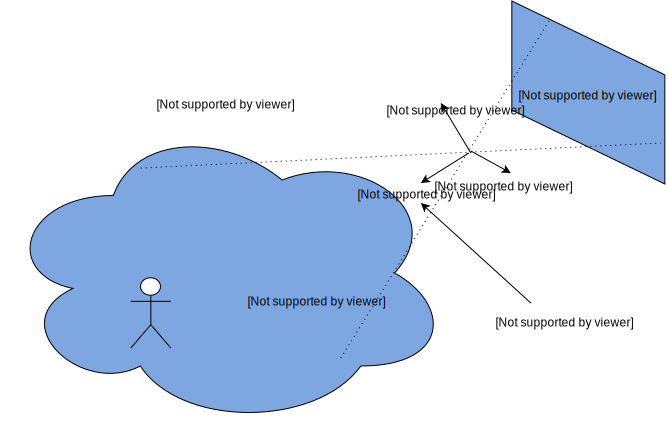
\includegraphics[width=12cm]{./pictures/videoMonitoring}
%	\caption{Sistema di monitoraggio video}
%	\label{fig:videoMonitoring}
%\end{figure}
%\noindent 
%La posizione e l'orientamento della camera determinano l'\textit{\gls{inquadratura}} della scena.
%L'acquisizione, da parte della camera, della scena nell'istante di tempo $i$ viene definita \textit{immagine} o \textit{frame} i-esimo.
%La Figura \ref{fig:videoMonitoring} illustra questi concetti.\\
%Per semplificare l'analisi, considereremo immagini estratte in \textit{scala di grigi}.
%Quindi ciascuna immagine verr\`a rappresentata come una matrice di pixel, in cui ciascun elemento rappresenta l'intensit\`a luminosa (\textit{luma}) del pixel corrispondente.\\
%Nel seguito della trattazione useremo una specifica terminologia.
%Indicheremo con $\mathcal{X}$ l'insieme dei \textit{pixel} costituenti l'immagine acquisita dalla camera,
%\[ \mathcal{X} \subset \mathbb{N}^2, \]
%e con $x \in \mathcal{X}$ il singolo pixel.
%Quando vorremo considerare il frame acquisito all'istante di tempo $i$, useremo $z_i$, con $i=1,\dots , \infty$. 
%In particolare, per indicare il valore della \textit{luminosit\`a} del pixel $x$ per il frame $i$-esimo, useremo il termine $z_i(x)$, con 
%\[ z_i(x) \in [0, 255]. \]
\section{Rappresentazione digitale delle immagini}
\label{rappresentazImmagini}
Nel Paragrafo \ref{intrinsicParam} abbiamo introdotto il concetto di \textit{immagine digitale} come rappresentazione numerica dell'immagine bidimensionale.
	\begin{figure}[tb]
		\centering
		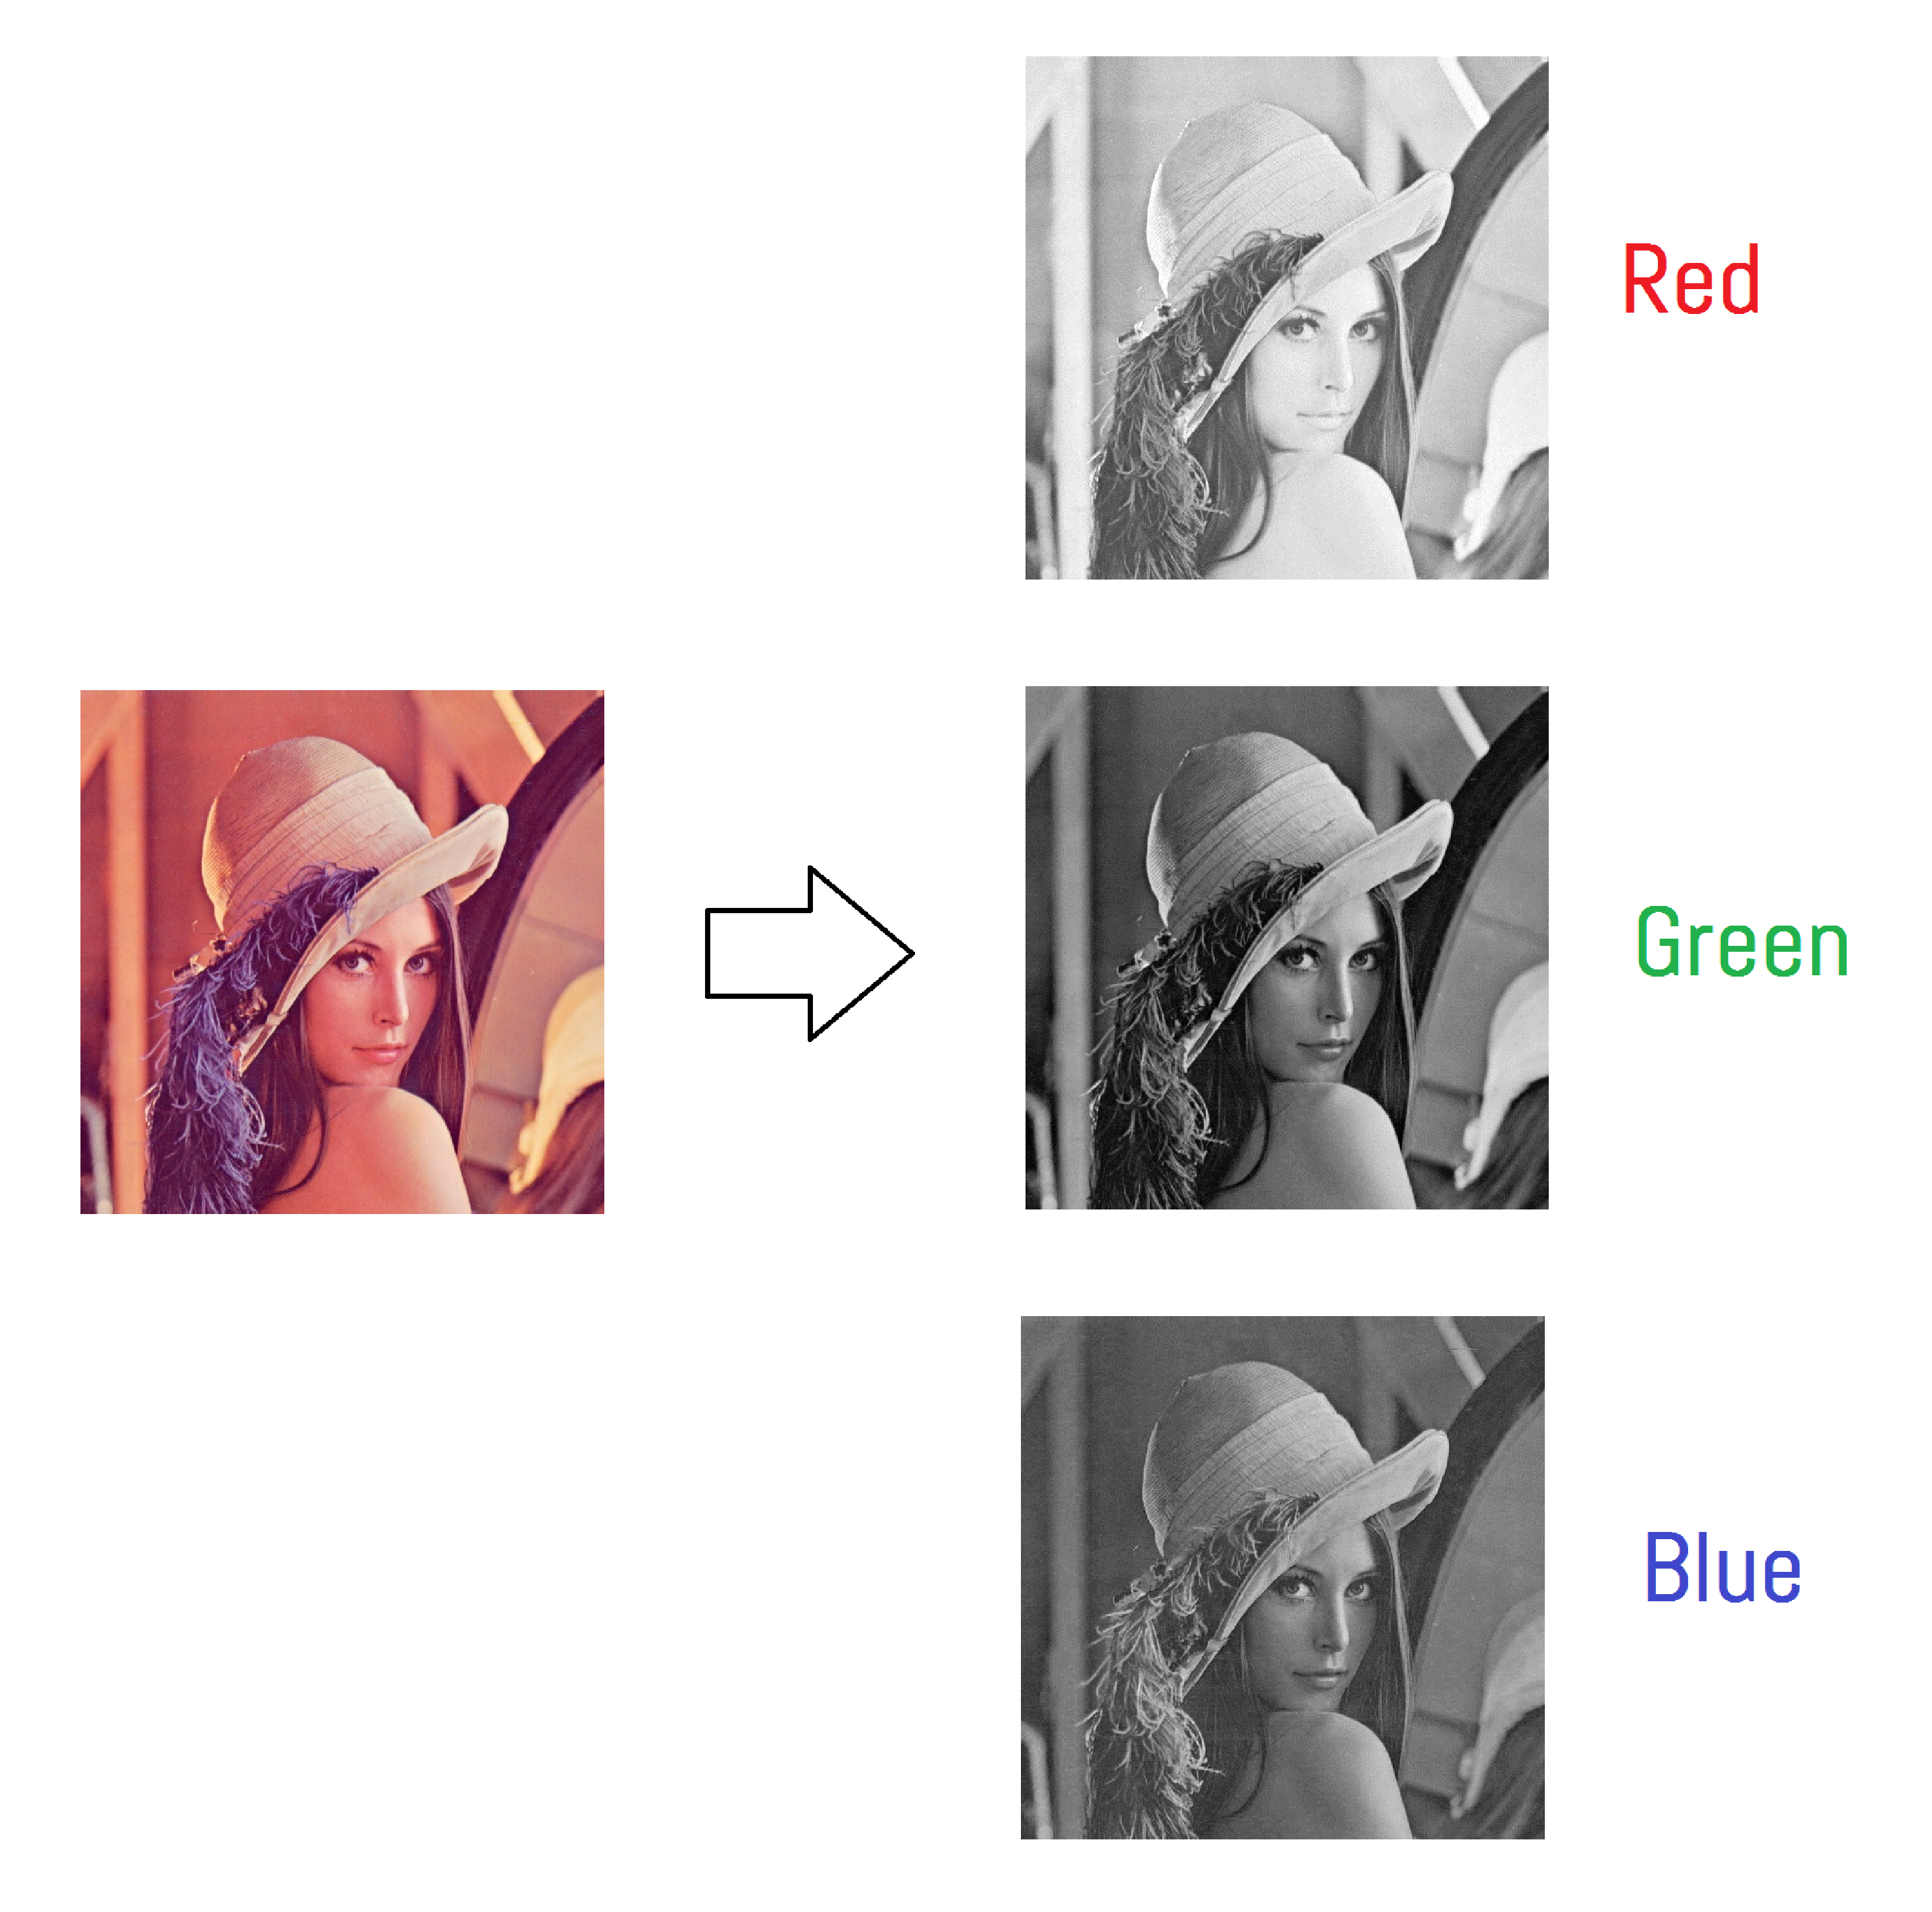
\includegraphics[width=8cm]{./pictures/lenaRGB}
		\caption{Esempio di estrazione dei canali RGB}
		\label{fig:lenaRGB}
	\end{figure}
Esistono vari modi di rappresentare un'immagine in formato digitale.
Le rappresentazioni che a noi interessa considerare sono \cite{forsyth2002computer}:
\begin{itemize}
	\item \textit{scala di grigi}, in cui l'immagine \`e rappresentata come una matrice $\textbf{I}$ di dimensioni $H \times W$, dove l'elemento $\textbf{I}(i,j)$ rappresenta il valore di \textit{intensit\`a luminosa} (\textit{luma}) del pixel di coordinate $(i, j)$;
	\item \textit{RGB}, dove l'immagine \`e rappresentata come una matrice \textit{tridimensionale} $\textbf{I}_{RGB}$ di dimensioni $H \times W \times 3$, in cui vengono memorizzati i livelli di intensit\`a luminosa dei tre colori fondamentali \textit{rosso} (R), \textit{verde} (G) e \textit{blu} (B) per ciascun pixel (Figura \ref{fig:lenaRGB}); 
	\item \textit{YUV}, in cui lo spazio colore viene definito tramite un componente di luma (Y) e due componenti di \textit{crominanza} (UV), che rappresentano rispettivamente i valori di differenza dal colore blu ($U = B - Y$) e dal colore rosso ($V = R - Y$) (Figura \ref{fig:yuv}).
\end{itemize}
Le immagini digitali possono essere memorizzate in diversi formati.
Spesso vengono utilizzati algoritmi di \textit{compressione}, che possono essere
\begin{itemize}
	\item a perdita di informazione (\textit{lossy}), come nel caso delle immagini \textit{JPEG};
	\item senza perdita di informazione (\textit{lossless}), come nel caso dei file d'immagine \textit{PNG} o \textit{GIF}.
\end{itemize}
	\begin{figure}[tb]
		\centering
		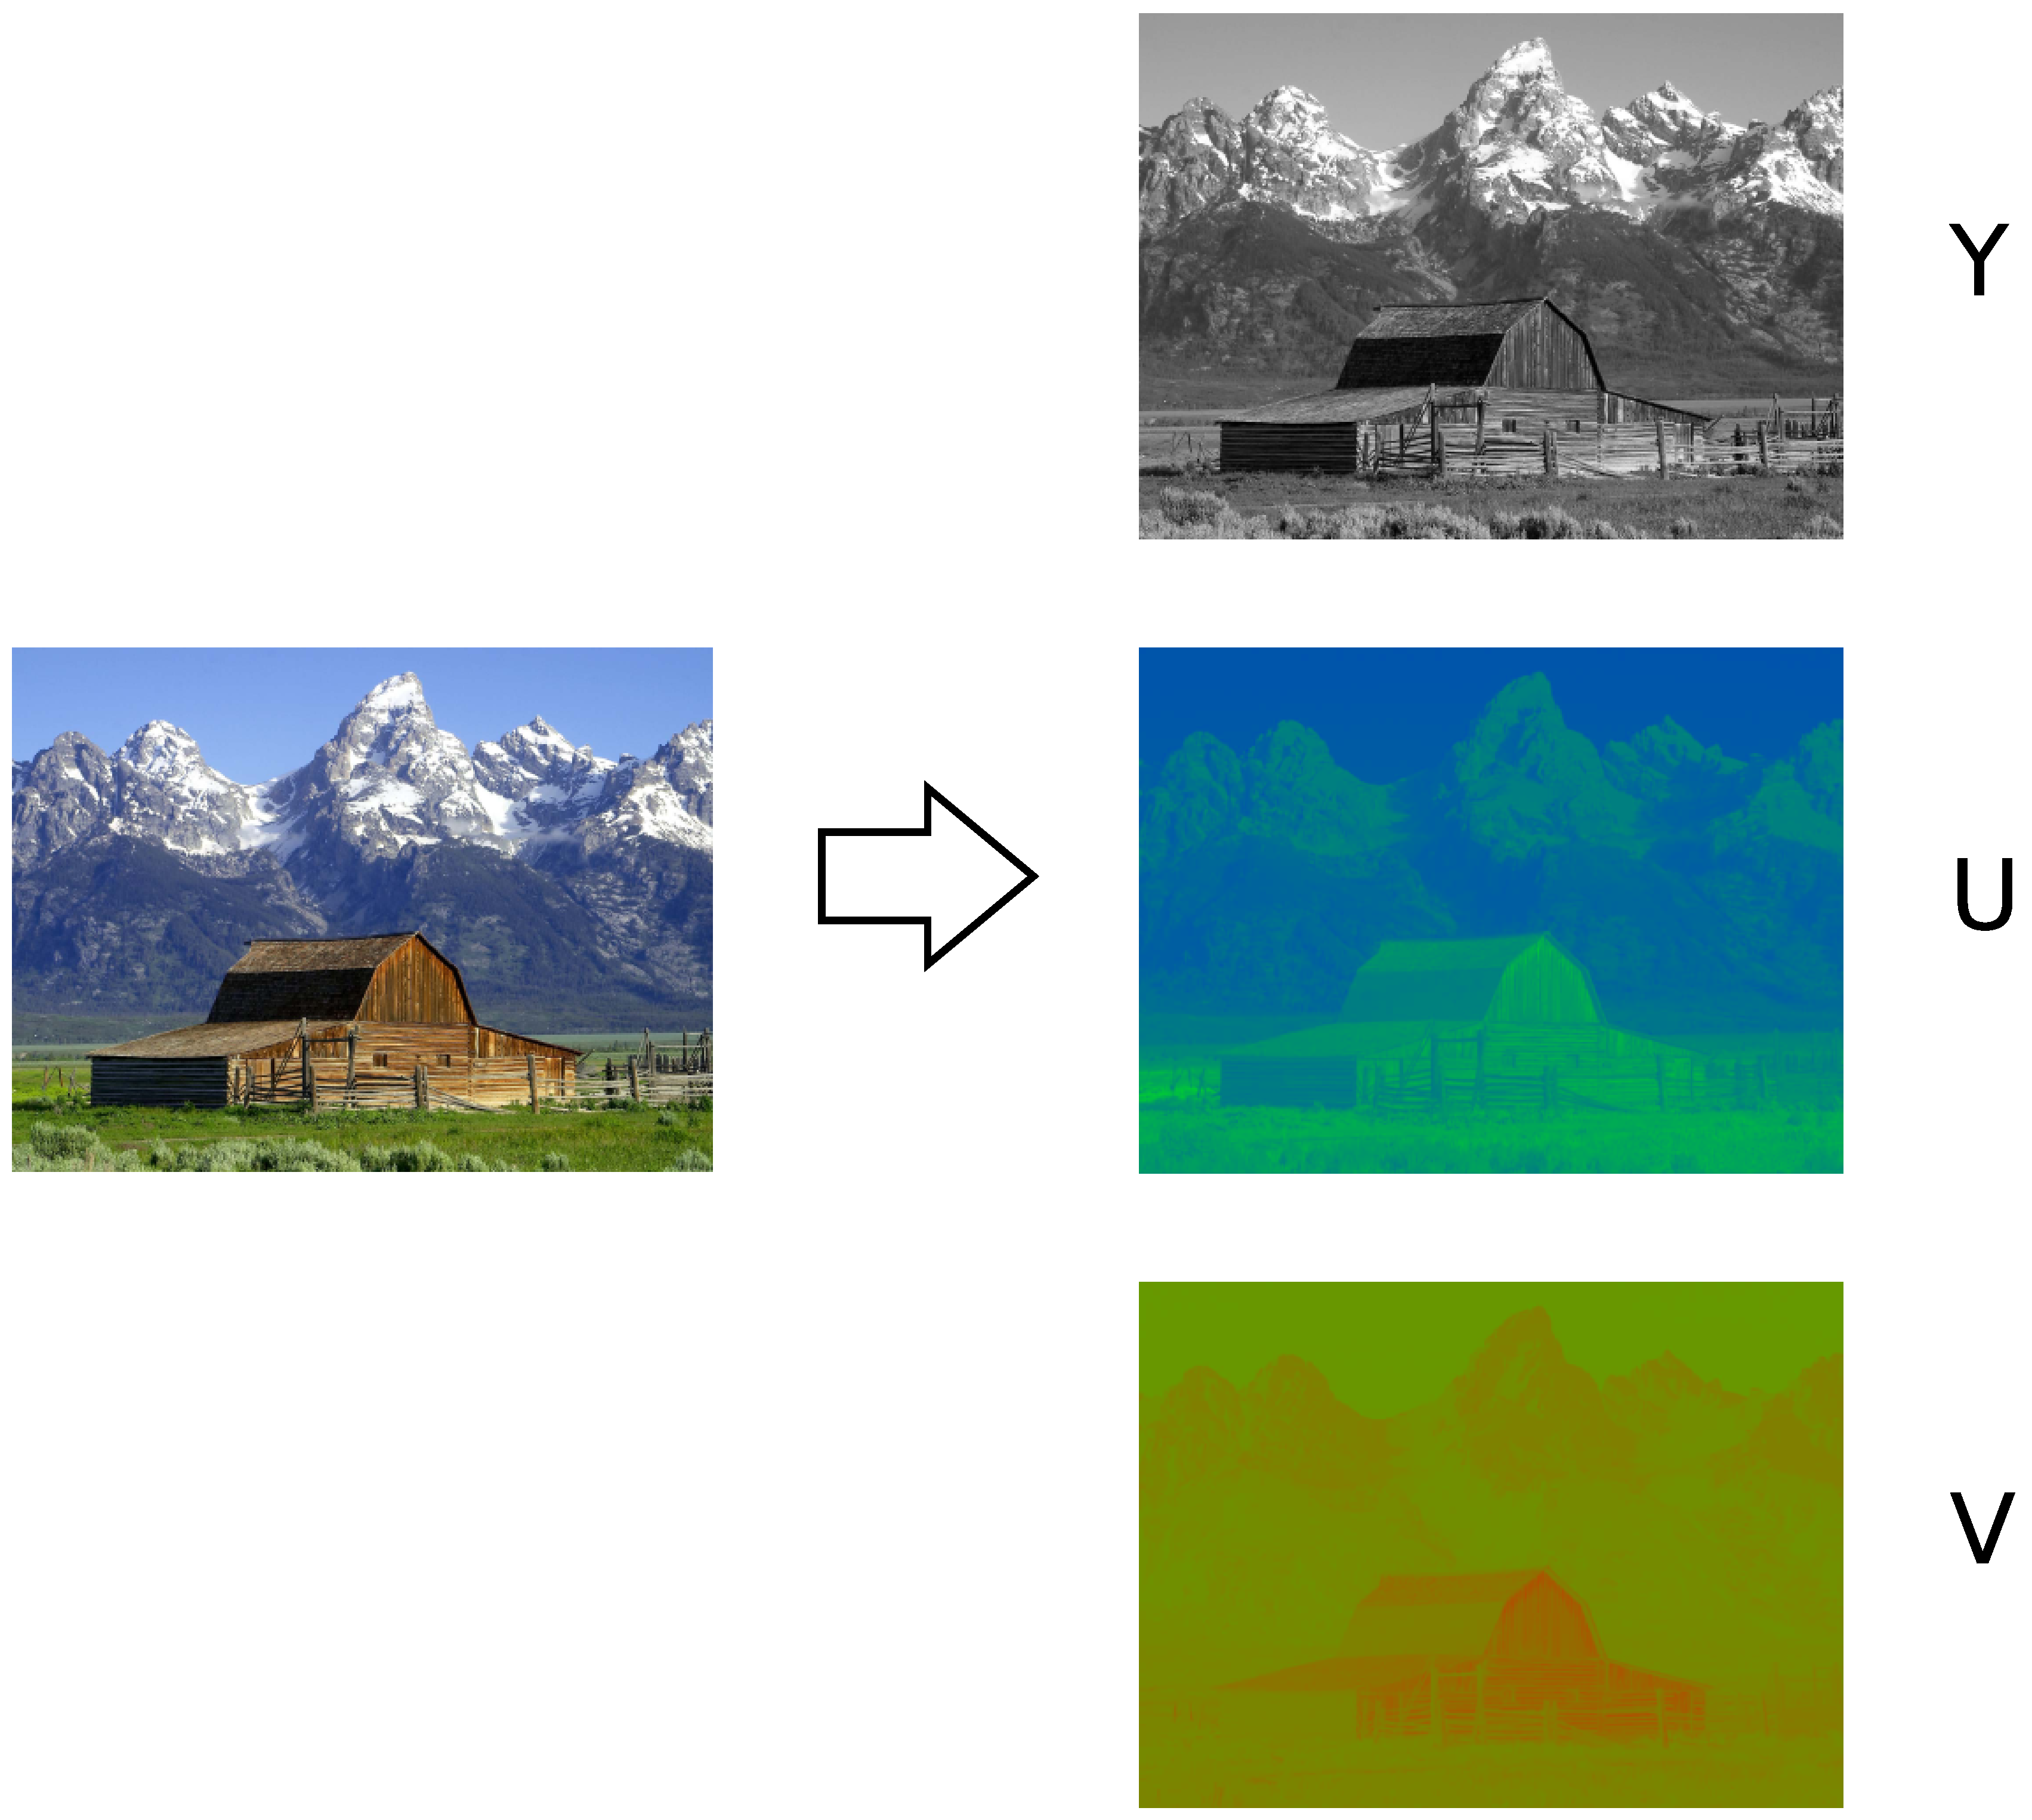
\includegraphics[width=8cm]{./pictures/yuv}
		\caption{Esempio di estrazione dei canali YUV}
		\label{fig:yuv}
	\end{figure}
	



\section{Identificazione del cambiamento nella stazionariet\`a di un processo}
\label{cdt}
Prima di illustrare come \`e stato affrontato il problema del tampering detection nella letteratura scientifica, affrontiamo il problema, pi\`u generale, di come identificare un cambiamento all'interno di un processo.
Una caratteristica, richiesta in molte applicazioni di analisi e elaborazione intelligente di dati, riguarda l'assunzione che il processo generante questi dati non cambi nel tempo \cite{alippi2014intelligence}. In questo caso si parla di processi \textit{stazionari}, ovvero processi in cui i dati possa no essere considerati generati da un'unica distribuzione probabilistica. \\
In molte situazioni, soprattutto se vengono utilizzati dei sensori per misurare delle grandezze fisiche, si pu\`o incorrere in situazioni in cui questa ipotesi di stazionariet\`a venga meno.
Ad esempio, pu\`o succedere che il sensore si guasti, oppure che fenomeni esterni non permettano un'acquisizione ottimale. 
In questi casi \`e opportuno avere a disposizione degli strumenti in grado di identificare quando la condizione di stazionariet\`a di un processo viene meno, in modo da poter lanciare un allarme a riguardo. 
Le tecniche principalmente utilizzate per questo scopo prendono il nome di \textit{Change-Point Methods} (CPM) e \textit{Change-Detection Tests} (CDT), e verranno illustrate nel resto del paragrafo.	
\subsection{Metodi di Change-Point}
I metodi di Change-Point (CPM) vengono utilizzati per ispezionare una certa sequenza di dati e verificare la sua stazionariet\`a. 
Ci\`o viene fatto verificando che, all'interno della sequenza, esista un istante temporale in cui la distribuzione dei dati cambia (\textit{change point}).\\
In maniera formale possiamo dire che, data una sequenza di dati
\[\mathcal{X}=\{x(t), t = 1,...,n\},\]
essa contiene un change point all'istante $\tau < n$ se \`e possibile
suddividerla in due sotto-sequenze
\[ \begin{array}{l}
\mathcal{A}_\tau = \{x(t), t = 1,...,\tau \}\\
 \mathcal{B}_\tau = \{x(t), t = \tau + 1,...,n \}
\end{array},\]
le quali sono due realizzazioni \textit{indipendenti e identicamente distribuite} (i.i.d.) di due differenti variabili aleatorie con distribuzione $ \mathcal{F}_0 $ e $ \mathcal{F}_1 $.
\`E possibile, quindi,  convertire il problema del change point in uno equivalente dove si valuta se $ \mathcal{A}_\tau $ e $ \mathcal{B}_\tau $ sono generati da due distribuzioni diverse.\\
Il problema, a questo punto, pu\`o essere riformulato come un \textit{test d'ipotesi a due campioni} \cite{ross2009introduction}, dove l'\textit{ipotesi nulla} ($ H_0 $) e l'\textit{ipotesi alternativa} ($ H_1 $) sono le seguenti:
\[ \begin{array}{rcl}
H_0: &  x(t) \sim &  \mathcal{F}_0 \quad  \forall t \\
H_1: &  x(t) \sim &
\begin{cases}
\mathcal{F}_{0} & \text{se } t < \tau \\
\mathcal{F}_{1} & \text{se } t \geq \tau
\end{cases}
\end{array}. \]
Per la valutazione delle ipotesi fatte sopra, occorrono delle opportune \textit{statistiche di test a due campioni} 
\[ \mathcal{T}_\tau = \mathcal{T}(\mathcal{A}_\tau, \mathcal{B}_\tau), \]
in modo da poter comparare $ \mathcal{A}_\tau $ e $ \mathcal{B}_\tau $. In questo modo \`e possibile rifiutare l'ipotesi nulla quando il valore della statistica $ \mathcal{T}_\tau $ supera una certa soglia $ h_{n,\alpha} $, calcolata in funzione di un certo \textit{intervallo di confidenza} $ \alpha $ e del numero di campioni $ n $.\\
Se, ad esempio, consideriamo l'ipotesi che $
\mathcal{A}_\tau $
e $ \mathcal{B}_\tau $ siano generate da due
distribuzioni \textit{gaussiane}, \`e
possibile valutare la dissimilarit\`a tra le
due distribuzioni controllando i due
\textit{valori attesi}. Possiamo usare, come
statistica di test, la \textit{differenza
	standardizzata tra le medie di due
	campioni}, definita come
\[ D_\tau = \sqrt{\frac{\tau(n-\tau)}{n}}
\frac{\overline{\mathcal{A}}_\tau-\overline{\mathcal{B}}_\tau}{S_\tau}, \]
dove $ \overline{\mathcal{A}}_\tau $ e $ \overline{\mathcal{B}}_\tau $ denotano le \textit{medie campionarie} valutate rispettivamente su $ \mathcal{A}_\tau $ e $ \mathcal{B}_\tau $, mentre $ S_\tau $ \`e la \textit{varianza campionaria} valutata \textit{su tutto l'insieme dei dati}.\\
Quando la statistica di test utilizzata,
corrispondente a una specifica partizione
dell'insieme dei dati, non fornisce l'evidenza
necessaria a rifiutare $ H_0, $ l'unica cosa
che \`e possibile stabilire \`e che
nell'istante $ \tau $ scelto non si \`e avuto
un cambiamento nella stazionariet\`a
dell'insieme. \textit{Ci\`o non implica che	l'istante di cambiamento non sia un altro ancora da valutare.} 
In maniera rigorosa \`e necessario valutare, quindi, tutte le possibili partizioni dell'insieme dei dati considerati. 
Le ipotesi nulla e alternativa vengono, perci\`o, modificate nel seguente modo \cite{ross2011nonparametric}:
\[
\begin{array}{rccl}
H_0 :& \forall t, & x(t) \sim & \mathcal{F}_0 \\
H_1 :& \exists \tau & x(t) \sim &
\begin{cases}
\mathcal{F}_{0} & \text{se } t < \tau \\
\mathcal{F}_{1} & \text{se } t
\geq \tau
\end{cases}
\end{array}.
\]
Entrando pi\`u nel dettaglio, per ciascun
punto $ s \in \{2,...,n-1\} $, candidato a
essere un change point, valutiamo la
statistica di test $ \mathcal{T}_s. $ Viene scelto come
change point quello che massimizza la
statistica
\[ M= \argmax_{s=2,...,n-1} (\mathcal{T}_s), \]
corrispondente al valore $ \mathcal{T}_M $ di $\mathcal{T}$
\[ \mathcal{T}_M = \max_{s=2,...,n-1} (\mathcal{T}_s).\]
Una volta trovato $\mathcal{T}_M$ il test va finalizzato
comparando questa statistica con la soglia
$ h_{n,\alpha}, $ in modo da verificare se
l'ipotesi nulla sia da scartare o meno.
\begin{figure}[tb]
	\centering
	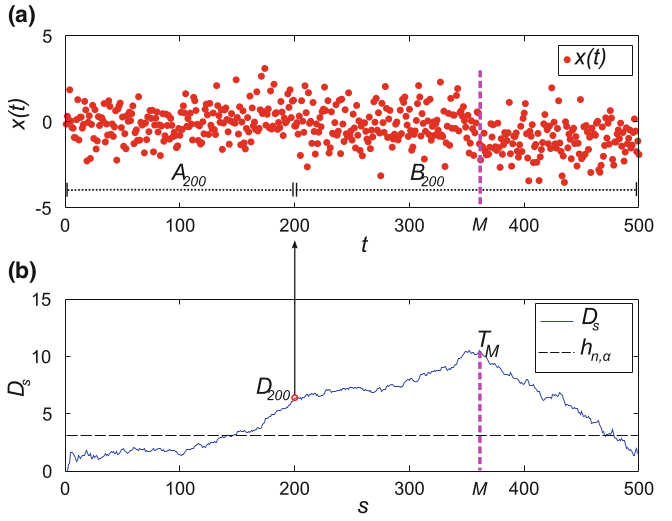
\includegraphics[width=12cm,keepaspectratio]{pictures/CPM}
	\caption[Esempio di CPM]{Un esempio di CPM basato sulla statistica $t$ di Student. I dati in (a) sono distribuiti in accordo con \eqref{eq:esempioCPM}. I valori assunti dalla corrispondente statistica di test ${D_s,s=2,\dots,499}$ sono riportati in (b). Sono riportati anche il change point stimato $M$, e il corrispondente valore nella statistica di test $\mathcal{T}_M$. A scopo illustrativo la figura mostra anche  la partizione di $\mathcal{X}$ in $\mathcal{A}_s$ e $\mathcal{B}_s$ quando $s=200$, insieme al corrispondente valore della statistica $D_{s=200}$.}
	\label{fig:CPM}
\end{figure}
Nella Figura \ref{fig:CPM} possiamo vedere un esempio di CPM basato su una statistica \textit{t di Student} \cite{alippi2014intelligence}. La sequenza \`e formata da 500 dati (\textbf{a}) ed \`e stato individuato un cambiamento un cambiamento nella loro distribuzione all'istante $\tau=350$:
\begin{equation}
	\label{eq:esempioCPM}
	x(t)\sim \left\{ \begin{array} {lcl}
	\mathcal{N}(0,1) & \mbox{, se} & t< 350 \\
	\mathcal{N}(-1,1) & \mbox{, se} & t\geq 350 \end{array} \right. .
\end{equation} 
I valori delle varie statistiche in funzione di s sono visualizzati in (\textbf{b}).\\
Spesso \`e preferibile utilizzare dei test
statistici \textit{non parametrici},
soprattutto quando le distribuzioni dei dati
sono incognite. Le statistiche maggiormente
utilizzate sono quelle basate su
\textit{calcolo del rango}
\cite{ross2011nonparametric}. Quando si ha a
che fare con cambiamenti nella
\textit{localit\`a} dei dati una statistica
solitamente utilizzata \`e quella di
\textit{Mann-Whitney}, mentre quando si
vogliono verificare cambiamenti \textit{di
	scala} \`e possibile utilizzare la
statistica di \textit{Mood}. La statistica di
\textit{Lepage} invece pu\`o risultare utile
per analizzare entrambi i tipi di
cambiamento. Un altro approccio consiste nel
comparare le \textit{distribuzioni empiriche}
dei due insiemi di dati, usando ad esempio la
statistica di \textit{Kolmogorov-Smirnov}.
\subsection{Change-Detection Test}
I metodi di change point sono stati principalmente
pensati per essere eseguiti \textit{a valle} della
completa acquisizione dei dati. Inoltre il suo elevato
costo computazionale fa s\`i che questa tecnica
difficilmente possa essere utilizzabile all'interno di
un sistema embedded. Le tecniche che vengono descritte
in questo paragrafo, che prendono il nome di
\textit{change detection test} (CDT), hanno come scopo
principale quello di fare un'elaborazione dei dati
\textit{online}, ovvero non appena questi sono
disponibili. Tecniche di questo tipo vengono anche
chiamate \textit{sequenziali}. La loro
relativa semplicit\`a dal punto di vista
computazionale permette di utilizzarle all'interno di
sistemi embedded ma, rispetto alle tecniche basate su
CPM, abbiamo una latenza (ovvero l'intervallo di tempo
tra l'istante di identificazione del cambiamento e
quello in cui effettivamente questo \`e avvenuto) e un
numero di falsi positivi (viene segnalato un
cambiamento nella distribuzione quando in, realt\`a,
questo non \`e avvenuto) maggiori.
\subsubsection{CDT basati su CUSUM}
Le \textit{carte di controllo per le somme cumulate} (CUMulative SUM control chart, abbreviate in \textit{CUSUM}) \cite{alippi2014intelligence,ross2009introduction} permettono di identificare un cambiamento all'interno di una sequenza di dati in maniera molto accurata utilizzando alcune informazioni \textit{a priori} sul processo generante i dati. Queste informazioni vengono generalmente acquisite durante un \textit{fase di configurazione} del test, in modo da fissare i parametri di test necessari all'analisi.\\
Nel seguito presentiamo due metodi di CDT che
estendono il metodo CUSUM tradizionale rilassando
alcune delle sue assunzioni troppo restrittive.  La
prima variante permette di identificare in maniera
automatica la configurazione dei parametri di test
(\textit{CUSUM adattativo}), mentre la seconda,
chiamata \textit{computational Intelligence CUSUM}
(CI-CUSUM) \`e in grado di considerare un insieme
pi\`u ricco di descrittori in modo da aumentare
l'efficienza nell'identificare i cambiamenti
\cite{alippi2008just}.  
\subparagraph{CUSUM tradizionale e versione adattativa}
Sia \[\mathcal{X}=\{x(t),t=1,...,N\},x(t)\in \mathbb{R}\]
una sequenza di $N$ dati generata da un processo con
densit\`a probabilistica $f_\theta(x)$, che assumiamo
sconosciuta e parametrizzata secondo un vettore
$\theta\in\mathbb{R}^n$. Assumiamo, inoltre, che il
processo cambi la sua stazionariet\`a a un istante
$T^0$ sconosciuto. Questo avvenimento pu\`o essere
modellato come un passaggio dal vettore dei parametri
$\theta_0$ a $\theta_1$, associati rispettivamente
alle densit\`a $f_{\theta_0}(x)$ e
$f_{\theta_1}(x)$. La discrepanza tra le due densit\`a
viene valutata comparando il rapporto tra le
log-verosimiglianze (\textit{log-likelihood ratio})
\[
s(t)=ln\frac{f_{\theta_1}(x(t))}{f_{\theta_0}(x(t))}
\textit{ per ogni } t=1,...,N \]
e la \textit{somma cumulata}
\[ S(t) = \sum^t_{\tau=1} s(\tau) \]
CUSUM identifica un cambiamento in $\mathcal{X}$ all'istante $\widehat{T}$ quando \[g(t)=S(t)-m(t),\] ovvero la differenza tra il valore della somma cumulata all'istante $t$ e il suo valore minimo nel tempo \[m(t)=\min_{\tau=1,...,t}S(\tau),\] supera una certa soglia $h$.\\
Il metodo CUSUM tradizionale assume che i parametri $\theta_0$, $\theta_1$ e la soglia $h$ siano disponibili a priori. La versione adattativa viene incontro a questa assunzione che, generalmente, \`e difficile da soddisfare.\\
La variante prima di tutto genera la sequenza cumulata
$Y=\{y(1),y(2),...\}$, dove $y(s)$ rappresenta il
valore della media campionaria stimata su una
\textit{finestra mobile non sovrapponibile} di
ampiezza $n$ presa da $\mathcal{X}$
\[ y(s) = \frac{1}{n} \sum_{t=(s-1)n+1}^{sn}x(t) \]
Scegliendo $n$ abbastanza grande, per il
\textit{teorema del limite centrale}
\cite{ross2009introduction}, la distribuzione di $Y$
pu\`o essere approssimata con una distribuzione
\textit{gaussiana}. In questo modo, quindi, si pu\`o
utilizzare il metodo CUSUM tradizionale direttamente
sulla sequenza $Y$. I primi $K$ dati di $\mathcal{X}$ vengono
usati come \textit{insieme di configurazione} per i
parametri necessari a identificare il cambiamento. Il
vettore dei parametri $\theta_0$ \`e caratterizzato da
media e varianza di $Y$, stimate attraverso i primi
$K/n$ campioni di $Y$. Il vettore dei parametri
$\theta_1$ viene ottenuto attraverso l'identificazione
di un intorno di confidenza per $\theta_0$, mentre la
soglia $h$ viene calcolata come il valore massimo di
$g(t)$ nella sequenza $Y$
\[ h=\max_{1\leq t\leq N/n}g(t). \]
\noindent L'intera procedura \`e illustrata nella
Figura \ref{fig:adaptiveCUSUM}.
\begin{figure}
	\centering
	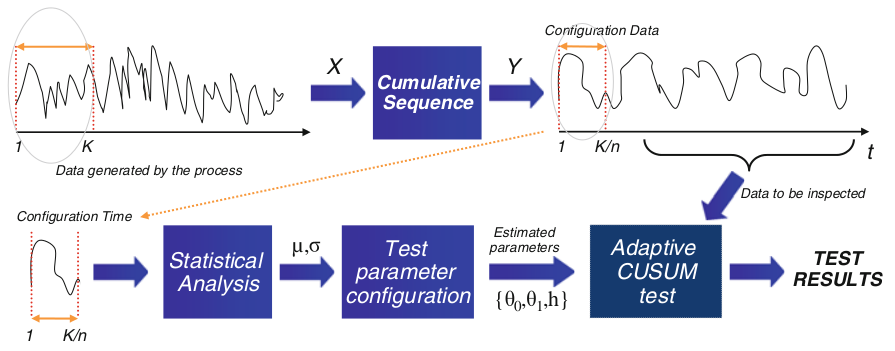
\includegraphics[width=12cm,keepaspectratio]{pictures/adaptiveCUSUM}
	\caption[Procedura del CUSUM
		adattativo]{Procedura del CUSUM
			adattativo. Il flusso di dati $\mathcal{X}$ passa attraverso un processo di fenestratura sequenziale. Non appena sono disponibili $n$ campioni in una finestra di dati questa viene utilizzata per generare l'indicatore $y(s)$, ottenuto tramite la media dei dati della finestra. La distribuzione di $y(s)$ \`e approssimativamente gaussiana, grazie al teorema del limite centrale, ammesso che $n$ sia abbastanza grande. Il CUSUM tradizionale pu\`o essere applicato sui parametri $\theta=[\mu,\sigma^2]$. I parametri $\theta_0,\theta_1$ e la soglia $h$ sono stimati sul insieme di training.}
	\label{fig:adaptiveCUSUM}
\end{figure}
\subparagraph{CI-CUSUM} Il metodo
CI-CUSUM rappresenta un'estensione del
CUSUM adattativo molto potente, in
quanto ciascun descrittore, estratto
dal flusso di dati, pu\`o essere
utilizzato per avere differenti gradi
di sensitivit\`a durante
l'identificazione di un cambiamento.
\begin{figure}
	\centering
	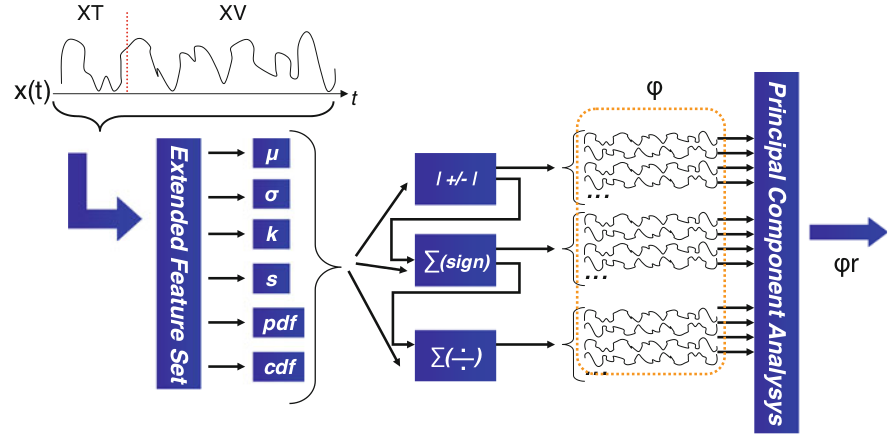
\includegraphics[width=12cm,keepaspectratio]{pictures/CI-CUSUM}
	\caption[Estrazione dei descrittori
		nel metodo CI-CUSUM]{Fase di estrazione dei descrittori e la fase di riduzione di CI-CUSUM. Un ampio insieme di descrittori viene estratto dal segnale in ingresso, in modo da comporre l'insieme descrittore $\varphi$. I descrittori estratti dall'insieme operazionale $XV$ sono comparati con quelli valutati nell'insieme di training $XT$. Una tecnica di analisi delle componenti principali permette la riduzione di $\varphi$ al descrittore $\varphi_r$.}
	\label{fig:CI-CUSUM}
\end{figure}
Facciamo riferimento alla Figura \ref{fig:CI-CUSUM}. I descrittori $\varphi$ considerati contengono i principali momenti della distibuzione dei dati, come media e varianza, ma anche momenti superiori al secondo come skewness (\textit{skew}) e kurtosis (\textit{kurt}), oltre che altre informazioni derivate dalla densit\`a probabilistica (\textit{pdf}) e dalla funzione di ripartizione dei dati (\textit{cdf}).\\
A ogni istante queste grandezze
vengono confrontate con quelle
appartenenti all'intervallo di
configurazione (\textit{training set},
indicato in Figura \ref{fig:CI-CUSUM}
come XT), in modo da valutare la
discrepanza tra questi valori. I
descrittori utilizzati sono
\[
\varphi_1(t)=|\mu_0-\mu_V|,\varphi_2(t)=|\sigma_0-\sigma_V|,\]
\[\varphi_3(t)=|\textit{kurt}_0-\textit{kurt}_V|,\varphi_4(t)=|\textit{skew}_0-\textit{skew}_V|, \]
\[\varphi_5(t)=\int_x|\textit{pdf}_0(x)-\textit{pdf}_V(x)|\textit{dx},\]
\[\varphi_6(t)=\int_x|\textit{cdf}_0(x)-\textit{cdf}_V(x)|\textit{dx}, \]
\[ \varphi_{7\leq j\leq 12}(t)=
\sum_{v=1}^{t-1}\textit{sgn}(\varphi_{j-6}(v+1)-\varphi_{j-6}(v)),\]
\[\varphi_{13\leq j\leq 24}(t)=
\sum_{v=1}^{t-1}\frac{\varphi_{j-12}(v+1)}{\varphi_{j-12}(v)} \]
In particolare, i descrittori
$\varphi_5(t)$ e $\varphi_6(t)$
valutano la discrepanza tra la
densit\`a e funzione di ripartizione
correnti e quelle rispettive
dell'intervallo di configurazione. I
descrittori da $\varphi_7(t)$ a
$\varphi_{12}(t)$ vanno ad analizzare
i cambiamenti di segno in elementi
consecutivi e quelli da
$\varphi_{13}(t)$ a $\varphi_{24}(t)$
la somma cumulata del rapporto tra
elementi consecutivi. Per ridurre la
complessit\`a dello spazio dei
descrittori viene applicata
un'\textit{analisi delle componenti
	principali} su $\varphi$, in modo da
avere la trasformata $\varphi_r$. A
questo punto, dato che la
distribuzione di $\varphi_r$ non \`e
nota a priori, viene applicato un
CUSUM adattativo su di essa.
\subsubsection{CDT basati su Intersezione di Intervalli di Confidenza}
La famiglia di tecniche che andiamo ad analizzare adesso \`e in grado di identificare cambi di stazionariet\`a, in un flusso di dati, monitorando l'evoluzione nel tempo di un certo numero di descrittori estratti dai dati stessi.
L'ipotesi principale che viene fatta \`e che le osservazioni della sequenza monitorata siano \textit{indipendenti e identicamente distribuiti} (\textit{i.i.d.}) e generati da una distribuzione \textit{gaussiana}.
\subparagraph{ICI-CDT}
In \textit{ICI-CDT} (Intersection of Confidence Intervals Change Detection Test) \cite{alippi2011just}, i descrittori sono estratti attraverso una \textit{fenestratura} dei dati disponibili in sotto-sequenze composte da $n$ istanze. Per ciascuna sotto-sequenza calcoliamo media e  varianza campionarie che, per il \textit{teorema del limite centrale} \cite{ross2009introduction}, possono essere considerate distribuite in maniera gaussiana. Entrando nel dettaglio, se consideriamo $s$ come l'\textit{s-esima} sotto-sequenza, i descrittori estratti sono:
\[ M(s)=\frac{\sum\limits_{t=(s-1)n+1}^{ns}x(t)}{n} \text{ , e } V(s)=\left(\frac{\sum\limits_{t=(s-1)n+1}^{ns}(x(t)-M(s))^2}{n-1}\right)^{h_0}, \]
dove il parametro $h_0$ \`e un esponente utilizzato per generare un'approssimazione gaussiana della varianza campionaria.\\
ICI-CDT utilizza una prima sequenza dei dati in cui si assume l'assenza di cambiamenti nella distribuzione. Tale sequenza prende il nome di \textit{insieme di training} e viene indicata con $O_{T_0}$. Da questa sequenza viene stimato il parametro $h_0$ e si configura il CDT. La configurazione avviene attraverso le due sequenze di descrittori $\{M(s), s=1,...,S_0\}$ e $\{V(s), s=1,...,S_0\}$, con $S_0=T_0/n$.\\
Calcoliamo quindi le medie $\widehat{\mu}^M_{S_0}$, $\widehat{\mu}^V_{S_0}$ e le deviazioni standard $\widehat{\sigma}^M_{S_0}$, $\widehat{\sigma}^V_{S_0}$ dei descrittori nell'insieme di training, ovvero:
\[ \widehat{\mu}^M_{S_0}=\frac{\sum\limits_{s=1}^{S_0}M(s)}{S_0} \text{ , e } \widehat{\sigma}^M_{S_0}=\sqrt{\frac{\sum\limits_{s=1}^{S_0}(M(s)-\widehat{\mu}^M_{S_0})^2}{S_0-1}}, \]
e
\[ \widehat{\mu}^V_{S_0}=\frac{\sum\limits_{s=1}^{S_0}V(s)}{S_0} \text{ , e } \widehat{\sigma}^V_{S_0}=\sqrt{\frac{\sum\limits_{s=1}^{S_0}(V(s)-\widehat{\mu}^V_{S_0})^2}{S_0-1}}. \]
Queste stime definiscono gli \textit{intervalli di confidenza} per i descrittori media e deviazione standard che, sotto la condizione di stazionariet\`a, sono definiti come:
\[I_{S_0}^M= \left[\widehat{\mu}^M_{S_0}-\Gamma \widehat{\sigma}^M_{S_0} \text{, } \widehat{\mu}^M_{S_0}+\Gamma \widehat{\sigma}^M_{S_0}\right], \]
\[I_{S_0}^V= \left[\widehat{\mu}^V_{S_0}-\Gamma \widehat{\sigma}^V_{S_0} \text{, } \widehat{\mu}^V_{S_0}+\Gamma \widehat{\sigma}^V_{S_0}\right], \]
dove $\Gamma>0$ \`e un parametro che controlla l'ampiezza dell'intervallo di confidenza e, quindi, la probabilit\`a che un descrittore appartenga all'intervallo sotto l'ipotesi di stazionariet\`a. \\
Una volta che la fase di training viene completata, ICI-CDT diventa operativo e pu\`o essere utilizzato per identificare cambiamenti nella stazionariet\`a del flusso di dati. Non appena sono disponibili $n$ dati, viene creata una nuova sequenza $s$ e si calcolano i descrittori che andranno a popolare gli intervalli $I_{s}^{M}$ e $I_{s}^{V}$.\\
A questo punto \`e possibile applicare la \textit{regola dell'intersezione degli intervalli di confidenza} (ICI-rule) \cite{goldenshluger1997spatially}. Questa regola verifica se una nuova istanza di un descrittore possa essere intesa come una realizzazione della gi\`a esistente distribuzione gaussiana. Se ci\`o non viene verificato, allora \`e avvenuto un cambiamento nella distribuzione.\\
Da un punto di vista operazionale, per ciascuna sequenza $s$ vengono calcolati gli intervalli di confidenza dei descrittori come \`e stato fatto per quelli dell'insieme di training. ICI-CDT individua un cambiamento all'interno della sotto-sequenza $\widehat{s}$ se
\[\bigcap_{s<\widehat{s}}I_s^M \neq \varnothing \text{ e } \bigcap_{s\leq\widehat{s}}I_s^M = \varnothing \]
oppure
\[\bigcap_{s<\widehat{s}}I_s^V \neq \varnothing \text{ e } \bigcap_{s\leq\widehat{s}}I_s^V = \varnothing \]
e il tempo di identificazione $\widehat{T}=n\widehat{s}$ corrisponde all'ultimo termine della sotto-sequenza $\widehat{s}$.\\
\begin{figure}
	\centering
	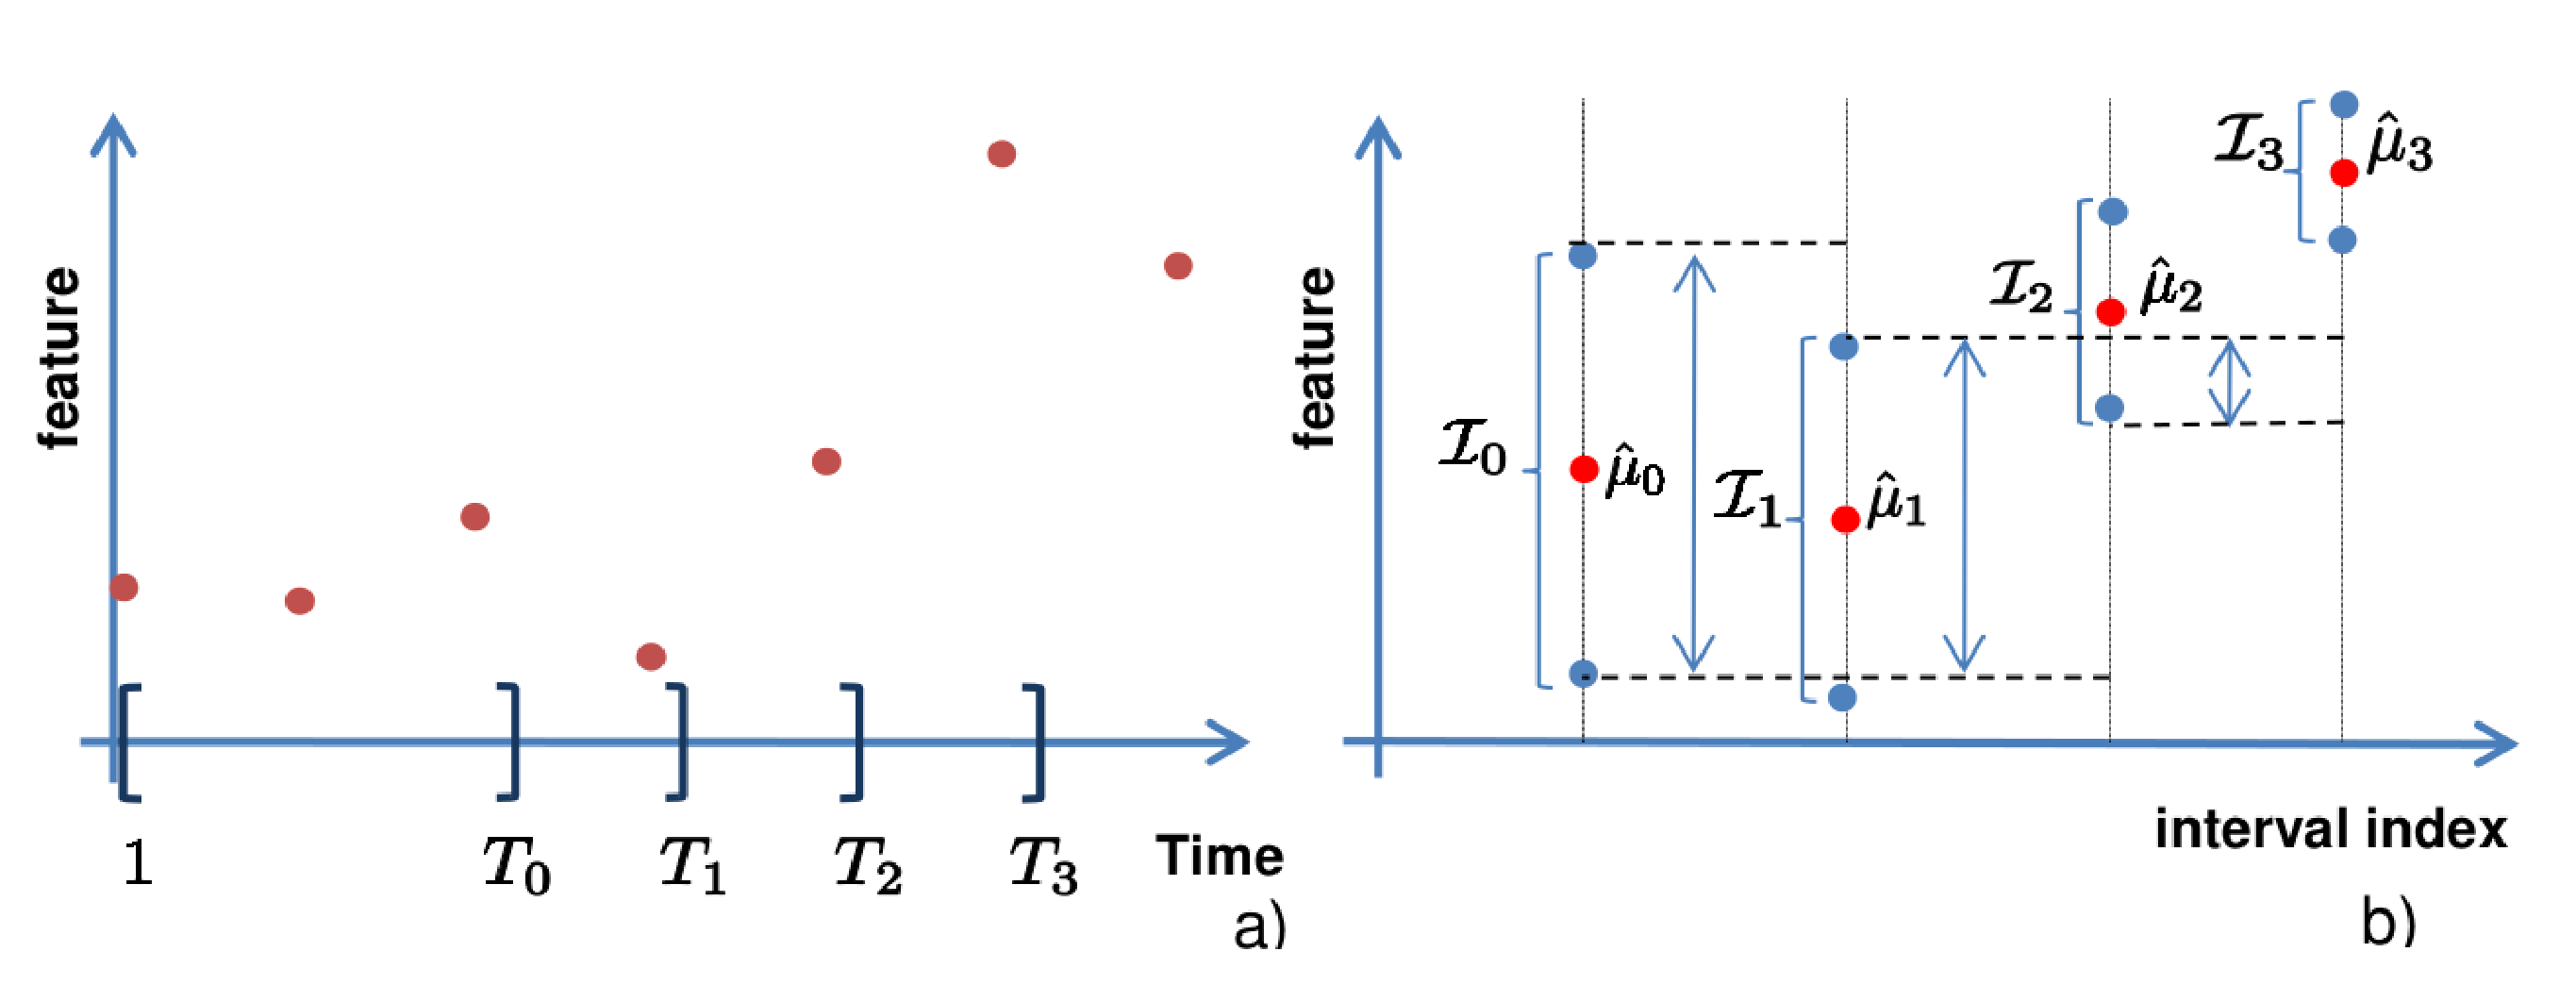
\includegraphics[width=12cm,keepaspectratio]{pictures/ICIrule}
	\caption[Esempio di come opera la regola dell'intersezione degli intervalli di confidenza (ICI-rule)]{Un esempio illustrativo di utilizzo di ICI-rule nella configurazione utilizzata per fare change detection: in (a) sono illustrati i valori del descrittore e l'insieme di intervalli $\{[1,T_0],[1,T_1],[1,T_2],[1,T_3]\}$, mentre in (b) vediamo i corrispondenti polinomi di ordine zero stimati, ei loro intervalli di confidenza. ICI-rule selezione l'intervallo $[1,T_2]$, dato che $\mathcal{I}_0\cap\dots\cap\mathcal{I}_2\neq\emptyset$ e $\mathcal{I}_0\cap\dots\cap\mathcal{I}_3=\emptyset$. Le parentesi graffe in (b) rappresentano gli intervalli di confidenza; le frecce invece rappresentano le loro intersezioni.}
	\label{fig:ICIrule}
\end{figure}
La Figura \ref{fig:ICIrule} illustra un esempio di come opera ICI-rule.\\
In \textbf{a} vengono rappresentati i valori dei descrittori e l'insieme di intervalli $\{[1,T_0], [1,T_1], [1,T_2], [1,T_3]\}$, mentre in \textbf{b} sono illustrati gli stimatori delle medie e i loro intervalli di confidenza. In questo caso ICI-rule individua un cambiamento nell'intervallo $[1,T_2]$, dato che $I_0 \cap ...\cap I_2 \neq \varnothing$ e $I_0 \cap ...\cap I_3 = \varnothing$.\\
Il principale problema di questa tecnica consiste nella sua \textit{intrinseca} latenza, dovuta al fatto che opera a finestre. 
Per risolvere questo limite \`e possibile applicare delle trasformazioni sui dati in modo da renderli approssimativamente gaussiani. Le trasformazioni pi\`u utilizzate sono quelle di \textit{Box-Cox}   \cite{box1964analysis}, per dati positivi, e di \textit{Manly}, \cite{manly1976exponential} che pu\`o essere utilizzato anche per dati negativi. Usando questo tipo di trasformazioni possiamo evitare di lavorare a finestre e utilizzare un approccio \textit{elemento  per elemento} \cite{boracchi2014reconfigurable}.           
\subparagraph{CDT di tipo gerarchico} 
Un altro problema di ICI-CDT consiste nel fatto che esso genera un numero molto elevato di falsi positivi. Per fare in modo che questo numero si abbassi, impattando il meno possibile sul tempo di esecuzione, \`e possibile fare un CDT di tipo \textit{gerarchico} \cite{alippi2011hierarchical}, basato su due livelli:
\begin{itemize}
	\item Il primo livello \`e composto da ICI-CDT, e opera sequenzialmente su tutti i dati.
	\item Il secondo livello consiste in un test d'ipotesi statistico in grado di validare o rifiutare l'ipotesi di avvenuto cambiamento. Questo livello viene attivato ogni volta che viene identificato un cambiamento da ICI-CDT.
\end{itemize}
\begin{figure}
	\centering
	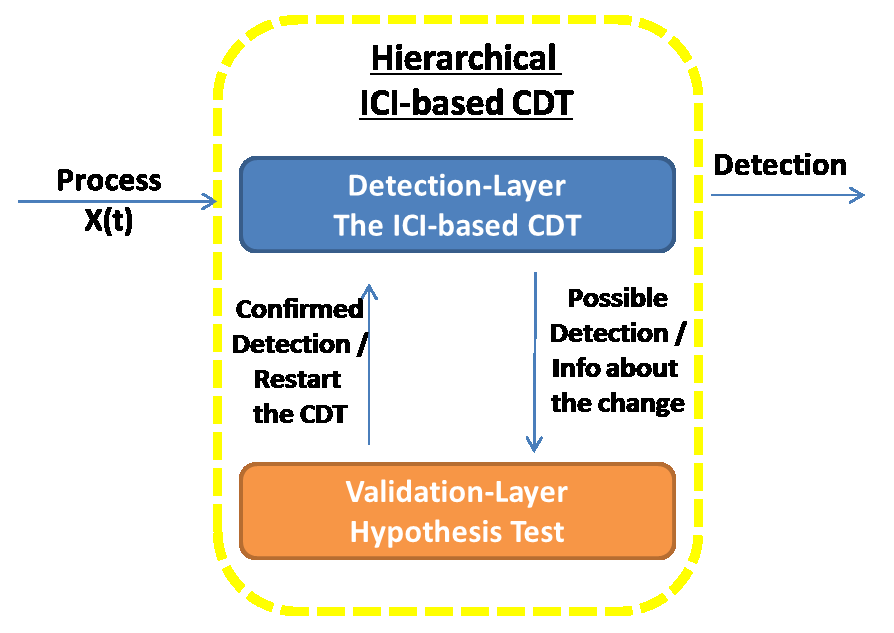
\includegraphics[width=8cm,keepaspectratio]{pictures/Hierarchical_ICI_based_CDT_Scheme}
	\caption{Schema del modo di operare del CDT di tipo gerarchico}
	\label{fig:HierarchicalCDT}
\end{figure}
Uno schema di come opera questo tipo di CDT \`e visualizzato nella Figura \ref{fig:HierarchicalCDT}.
Il CDT di tipo gerarchico \`e progettato in modo da avere un primo livello molto efficiente dal punto di vista del tempo di esecuzione, anche se ci\`o si traduce in un numero elevato di falsi positivi. Questo limite viene mitigato usando nel secondo livello della gerarchia un test pi\`u efficiente dal lato del numero di falsi positivi prodotti. Il fatto che il secondo livello ha un tempo di esecuzione maggiore non \`e un problema, in quanto esso viene attivato solamente nei casi in cui il primo livello della gerarchia segnala un possibile cambiamento nella distribuzione dei dati.
\section{Tampering Detection}
\label{tamperingSOA}
Nei moderni sistemi di videosorveglianza troviamo spesso algoritmi in grado di identificare particolari eventi all'interno della scena ripresa dalla camera. 
Ad esempio \`e possibile avere un software in grado di identificare le targhe delle automobili che superano il limite di velocit\`a, oppure la presenza di oggetti incustoditi in una stazione \cite{Targhe}.
Affinch\'e questi algoritmi funzionino correttamente, \`e importante che l'\textit{affidabilit\`a} del sistema di acquisizione sia preservata.
Questa propriet\`a viene soddisfatta quando:
\begin{itemize}
	\item la camera mantiene la stessa inquadratura nell'area di interesse;
	\item tutti gli elementi della scena sono distinguibili all'interno dell'immagine.
\end{itemize}
%In un'applicazione di monitoraggio video consideriamo che la camera, in condizioni di funzionamento ottimale, mantenga la stessa inquadratura nel tempo e che sia in grado di acquisire, in maniera nitida, tutti gli elementi di interesse presenti nella scena.
Definiamo \gls{tampering} un qualsiasi evento che determini un cambio di inquadratura o che non permetta la corretta acquisizione di una parte o della totalit\`a della scena.
Possiamo classificare gli eventi di tampering in quattro categorie:
\begin{itemize}
	\item sfocature,
	\item spostamenti della camera,
	\item occlusioni dell'obiettivo,
	\item guasti della camera.
\end{itemize}
La letteratura scientifica presenta molte tecniche in grado di affrontare il problema dell'identificazione di questo tipo di eventi.
%Per affrontare il problema dell'identificazione di questo tipo di eventi, la letteratura scientifica offre molte tecniche che permettano l'identificazione automatica di eventi in grado di compromettere la corretta ripresa della scena da parte della videocamera.
\begin{figure}[tb]
	\centering
	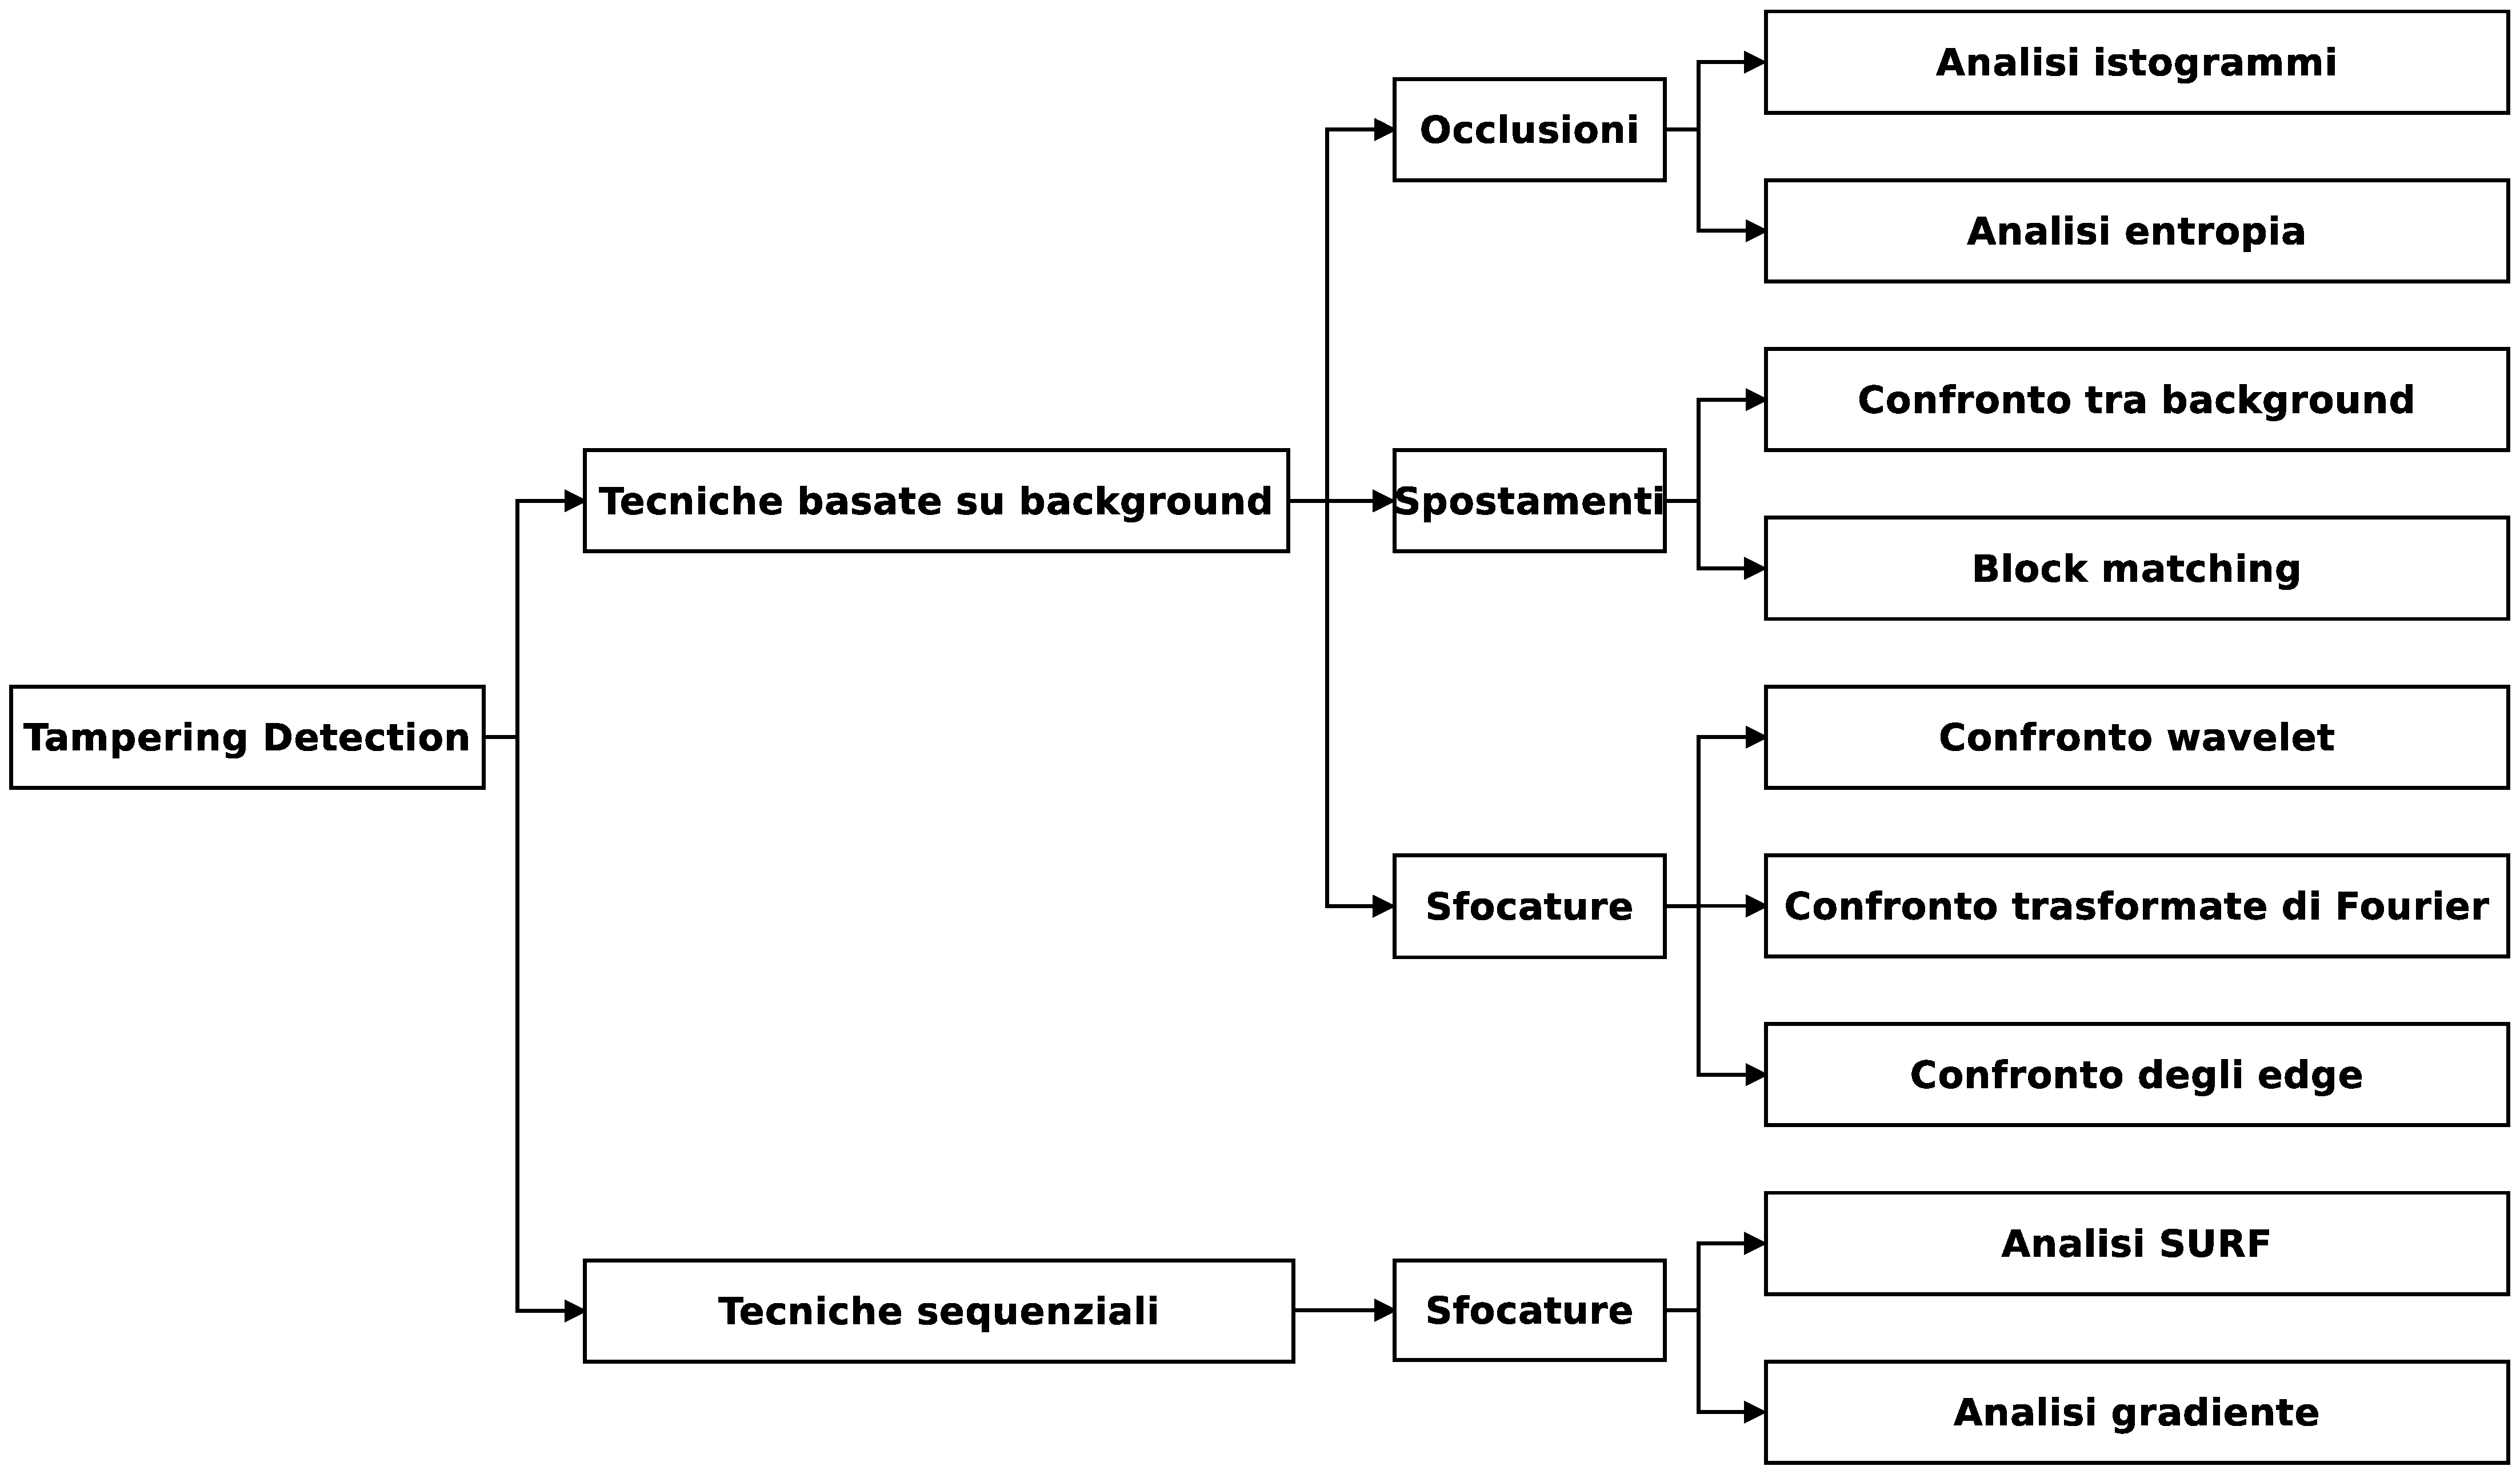
\includegraphics[width=12cm]{./diagrammi/tecnicheSOA.eps}
	\caption{Tecniche di tampering detection}
	\label{fig:tamperingSOA}
\end{figure}
Lo schema in Figura \ref{fig:tamperingSOA} mostra le principali tecniche di tampering detection presenti in letteratura.
Queste possono essere divise in due categorie: 
\begin{itemize}
	\item tecniche basate su confronto di background,
	\item tecniche basate su monitoraggio sequenziale.
\end{itemize}
Nel seguito del paragrafo verranno descritti i principali metodi utilizzati in queste due categorie.
\subsection{Concetti e terminologia}
\label{concetti}
Prima di concentrarci su come \`e stato affrontato il problema del tampering detection, definiamo i concetti e i termini che verranno utilizzati nel seguito della trattazione.\\
Lo scenario che consideriamo \`e quello di una camera che deve riprendere una particolare \textit{\gls{scena}}.
\begin{figure}[tb]
	\centering
	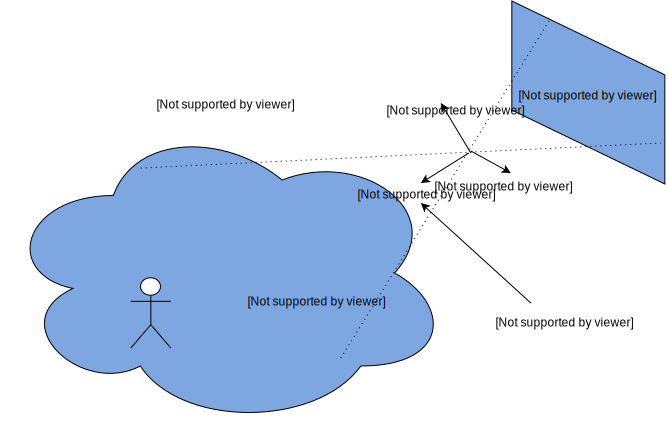
\includegraphics[width=12cm]{./pictures/videoMonitoring}
	\caption{Sistema di monitoraggio video}
	\label{fig:videoMonitoring}
\end{figure}
\noindent 
La posizione e l'orientamento della camera determinano l'\textit{\gls{inquadratura}} della scena.
L'acquisizione, da parte della camera, della scena nell'istante di tempo $t$ viene definita \textit{immagine} o \textit{frame} $t$-esimo.
La Figura \ref{fig:videoMonitoring} illustra questi concetti.\\
Per semplificare la trattazione, considereremo immagini estratte in \textit{scala di grigi}.
Ciascuna immagine, quindi, verr\`a rappresentata come una matrice di pixel, in cui ciascun elemento rappresenta l'intensit\`a luminosa (\textit{luma}) del pixel corrispondente.
L'estensione al caso di immagini \textit{RGB} \`e immediata: possiamo, infatti, applicare i vari algoritmi in maniera indipendente per ciascun canale di colore, per poi mediare i risultati ottenuti.\\
Nel seguito della trattazione useremo una specifica terminologia.
Indicheremo con $\mathcal{X}$ l'insieme dei \textit{pixel} costituenti l'immagine acquisita dalla camera,
\[ \mathcal{X} \subset \mathbb{N}^2, \]
e con $x \in \mathcal{X}$ il singolo pixel.
Quando vorremo considerare il frame acquisito all'istante di tempo $t$, useremo $z_t$, con $t=1,\dots , \infty$. 
In particolare, per indicare il valore della \textit{luminosit\`a} del pixel $x$ per il frame $t$-esimo, useremo il termine $z_t(x)$, con 
\[ z_t(x) \in [0, 255] \quad \forall x \in \mathcal{X}. \]

\subsection{Tecniche basate su confronto di background}
\label{background}
Nella maggior parte dei lavori dedicati al problema del tampering detection, il metodo principalmente utilizzato consiste nel confrontare ciascun frame con un modello che viene calcolato a partire dalle osservazioni precedenti.
Tale metodo \`e ampiamente utilizzato in vari ambiti della visione artificiale e prende il nome di \textit{background subtraction}.
Una tecnica generale di calcolo del background \`e presentata in \cite{aksay2007camera}.
%Indichiamo con $z_i(x)$ il valore, nel pixel $x$, della luminosit\`a nell'$i$-esimo frame.
Il valore del modello di background per il pixel $x$\ \`e calcolato, in maniera ricorsiva, secondo la seguente formula:
\[
\label{eq:background}
B_{t + 1}(x)=\left\{ \begin{array} {lcl}
aB_t(x)+ (1-a)z_t(x) \\
\mbox{\hspace{1.5cm}, se } |z_t(x) - z_{t-1}(x)|\leq T_t(x) \\
B_t(x) \mbox{\hspace{0.5cm}, se } |z_t(x) - z_{t-1}(x)|>T_t(x)\end{array} \right. , \forall x \in \mathcal{X},
\]
dove $0 < a < 1$ \`e chiamato \textit{parametro di aggiornamento} (\textit{update parameter}) e $\Gamma_t(x)$ \`e una soglia che permette di identificare un cambiamento sostanziale di luminosit\`a nel pixel $(x)$. 
 Questa soglia viene aggiornata in maniera ricorsiva secondo la seguente formula:
  \[
  \label{eq:backgroundThreshUpd}
  \Gamma_{t + 1}(x)=\left\{ \begin{array} {lcl}
  a\Gamma_t(x)+ (1-a)(c |z_t(x) - B_t(x)|) \\
  \mbox{\hspace{1.5cm}, se	}  |z_t(x) - z_{t-1}(x)|\leq \Gamma_t(x) \\
  \Gamma_t(x) \mbox{	\hspace{0.5cm}, se	}  |z_t(x) - z_{t-1}(x)|>\Gamma_t(x) \end{array} \right. ,\forall x \in \mathcal{X},
  \]
  dove $c > 1$ e $0<a<1$.
  Lo stesso modello viene utilizzato in altri lavori, come ad esempio in \cite{saglam2009real} e \cite{tsesmelis2013tamper}, mentre una variante molto usata consiste nel calcolare il modello di background a partire dall'\textit{estrazione dei contorni} di ciascun frame (\cite{harasse2004automated}, \cite{gil2007automatic}).
  Un approccio diverso, ma comunque riconducibile allo stesso filone, lo troviamo in \cite{ribnick2006real}, dove il background \`e sostituito da un \textit{buffer} contenente gli ultimi $n$ frame acquisiti dalla camera, che vengono confrontati con l'ultima osservazione per identificare eventi di tampering.
\subsubsection{Identificazione di occlusioni}
L'evento di occlusione avviene quando un oggetto opaco viene posto vicino alla camera, in modo da coprire la scena ripresa.
In \cite{aksay2007camera} e \cite{saglam2009real} questo evento \`e associato a un cambiamento nella struttura dell'\textit{istogramma} del frame occluso rispetto a quello del background.
In particolare, se $z_t$ \`e un frame in cui \`e avvenuta un'occlusione, ci si aspetta che il suo istogramma contenga i valori pi\`u alti in un intervallo pi\`u ristretto rispetto a quello del background $B_t$, in quanto la maggior parte dell'immagine prender\`a il colore dell'oggetto occludente o diventer\`a pi\`u scura.\\
Indichiamo con $H_b(\cdot)$ il valore del $b$-esimo bin dell'istogramma di un frame, con $1 \leq b \leq 32$.
Per identificare un evento di occlusione vengono considerate due disequazioni:
\begin{eqnarray}
 \left(H_{max\left(H(z_t)\right)-1}(z_t) + H_{max\left(H(z_t)\right)}(z_t) +  H_{max\left(H(z_t)\right) + 1}(z_t)\right) \nonumber \\
 > \Gamma_1 \left(H_{max\left(H(z_t)\right)-1}(B_t) + H_{max\left(H(z_t)\right)}(B_t)
  +  H_{max\left(H(z_t)\right) + 1}(B_t)\right), \nonumber
\end{eqnarray}
\[ \sum_{b=1}^{32} H_b\left(|z_t - B_t|\right) > \Gamma_2 \sum_{b=1}^{k}H_b\left(|z_t - B_t|\right),\]
dove $\Gamma_1 > 1$, $\Gamma_2 > 1$ e $0 \leq k < 32$ sono soglie che possono essere modificate in base alla sensibilit\`a che si richiede da parte dell'algoritmo.\\
%In particolare, $\Gamma_1$ e $\Gamma_2$ possono essere aumentate in modo da aumentare la sensibilit\`a, mentre $k$ pu\`o essere diminuito.\\
Un approccio simile \`e presente in \cite{harasse2004automated}, \cite{gil2007automatic} e \cite{ellwart2012camera}, in cui l'evento di occlusione \`e associato a un abbassamento dell'\textit{entropia}:
 \[
 \label{eq:entropy}
 E=-\sum_{k}p_k\ln(p_k) ,
 \]
 dove $p_k$ rappresenta la probabilit\`a che il livello di grigio $k$ sia presente all'interno dell'immagine. \\
 Per riuscire a identificare delle occlusioni \textit{parziali} le tecniche descritte sopra non sono efficaci, in quanto tali eventi non sono in grado di modificare in maniera sostanziale la struttura dell'istogramma dei frame.
 Una soluzione (\cite{gil2007automatic}) consiste nel dividere ciascuna immagine in un certo numero di \textit{blocchi} della stessa dimensione, in modo da applicare le tecniche descritte sopra per ciascuna partizione.
\subsubsection{Identificazione di spostamenti della camera}
Quando viene spostata la camera, in modo cambi l'inquadratura della scena, l'immagine di background $B_i$ viene lentamente aggiornato in modo da riflettere i cambiamenti avvenuti nei frame. 
In \cite{saglam2009real} il metodo proposto per identificare uno spostamento della camera consiste nel confrontare l'immagine di background $B_t$ con $B_{t-k}$, ovvero con un secondo modello \textit{ritardato} di $k$ frame, dove $k \in \mathbb{Z}^+$.
L'approccio consiste nel calcolare un \textit{valore di proporzione} $P$, ottenuto dal confronto tra i due modelli:
\[
\label{eq:displEqSaglam}
P=\left\{ \begin{array} {lcl}
P+1 & \mbox{, se} & B_t(x) \neq B_{t-k}(x) \\
P & \mbox{, se} & B_t(x) = B_{t-k}(x) \end{array} \right. .
\]
Lo spostamento della camera viene identificato quando $P > \Gamma \cdot K$, dove $0<\Gamma<1$ \`e un valore di soglia scelto in base alla sensibilit\`a che si vuole dare all'algoritmo e $K$ \`e il numero totale di pixel dell'immagine.\\
Un altro approccio \`e quello di utilizzare tecniche di \textit{block matching}.
L'algoritmo di block matching fornisce due parametri:
il primo parametro, $m$, indica il \textit{vettore della traslazione} tra il background e il frame corrente, mentre il secondo parametro \`e lo ZNCC relativo a quel vettore.
In \cite{harasse2004automated} e \cite{gil2007automatic} l'algoritmo calcola il vettore di spostamento $m$ del frame corrente rispetto al background, e calcola la \textit{zero-mean normalized cross correlation} (ZNCC) \cite{roma2002comparative}:
\[
ZNCC_t(m) = \frac{\sum_{x \in \mathcal{X}}(B_{t-1}(x)- \mu_{B_{t-1}})(z_t(x+m)-\mu_{z_t})}{\sigma_{B_{t-1}} \sigma_{z_t}},
\]
dove $\mu_{z_t}$ e $\sigma_{z_t}$ rappresentano la media e la deviazione standard della luminosit\`a nell'immagine $z_t$.
Lo spostamento viene individuato quando il vettore $m$ ha una lunghezza minima e lo ZNCC corrispondente supera una certa soglia.
Un metodo simile viene utilizzato anche in \cite{kryjak2012fpga}, con la differenza che, invece di analizzare la correlazione dei pixel, viene analizzata quella degli istogrammi. 
\subsubsection{Identificazione di sfocature} 
La conseguenza di un evento di sfocatura \`e la perdita di dettagli nell'immagine.
In \cite{aksay2007camera} e \cite{saglam2009real} questo fenomeno \`e associato a una diminuzione dell'energia ad alta frequenza. 
Per analizzare questo cambiamento, \cite{aksay2007camera} confronta ciascun frame con il background nel dominio delle \textit{wavelet} \cite{mallat1989theory}, mentre \cite{saglam2009real} utilizza il dominio della \textit{trasformata di Fourier} \cite{bracewell1978fourier}.
\begin{figure}[tb]
	\centering
	\begin{subfigure}[]
		{\label{fig:defocusNormale} 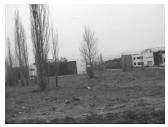
\includegraphics[width = 5cm]{./pictures/normale}}
	\end{subfigure}
	\begin{subfigure}[]
		{\label{fig:defocusNormaleFourier} 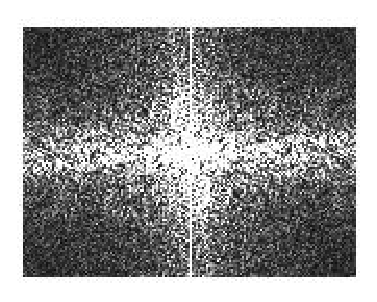
\includegraphics[width = 5cm]{./pictures/normale-fourier}}
	\end{subfigure}
	\begin{subfigure}[]
		{\label{fig:defocusSfocato} 
\includegraphics[width = 5cm]{./pictures/sfocato}}
	\end{subfigure}
	\begin{subfigure}[]
		{\label{fig:defocusSfocatoFourier} 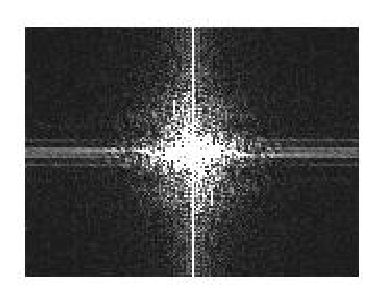
\includegraphics[width = 5cm]{./pictures/sfocato-fourier}}
	\end{subfigure}
	\caption{Comportamento della trasformata di Fourier nel caso di sfocatura}
	\label{fig:fourier}
\end{figure}
Nella Figura \ref{fig:fourier} vediamo un esempio di come si comporta la trasformata di Fourier nel caso di sfocature: 
nel passaggio da un frame nitido (Fig. \ref{fig:defocusNormale}) a uno sfocato (Fig. \ref{fig:defocusSfocato}) abbiamo un crollo delle componenti ad alta frequenza nelle trasformate di Fourier (rispettivamente Fig. \ref{fig:defocusNormaleFourier} e Fig. \ref{fig:defocusSfocatoFourier}).
L'evento di tampering viene individuato quando l'\textit{energia media} della trasformata di Fourier (o di quella wavelet) del frame corrente $E_{HF}(z_t)$ \`e $\Gamma$ volte minore di quella del background $E_{HF}(B_t)$:
\[E_{HF}(z_t)\leq \Gamma \cdot E_{HF}(B_t),\]
dove $0<\Gamma<1$ \`e  un valore di soglia scelto in base alla sensibilit\`a che si vuole dare all'algoritmo.\\
\begin{figure}[tb]
	\centering
	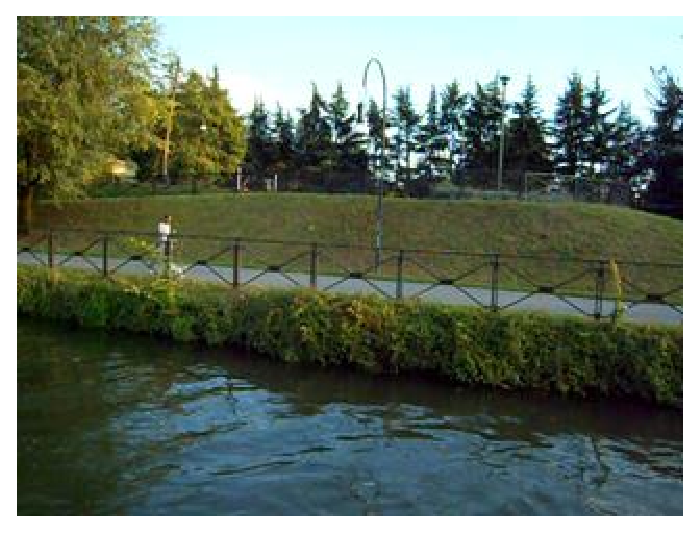
\includegraphics[width = 4cm]{./pictures/FPSalto/img0001}
	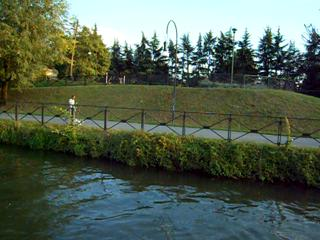
\includegraphics[width = 4cm]{./pictures/FPSalto/img0002}
	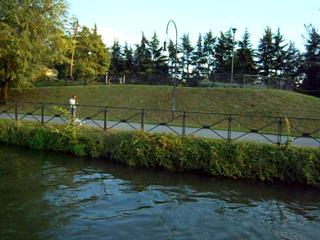
\includegraphics[width = 4cm]{./pictures/FPSalto/img0003}
	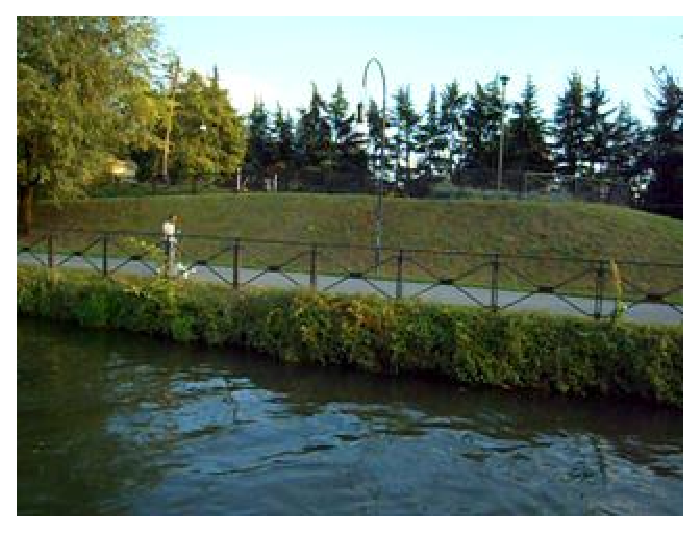
\includegraphics[width = 4cm]{./pictures/FPSalto/img0004}
	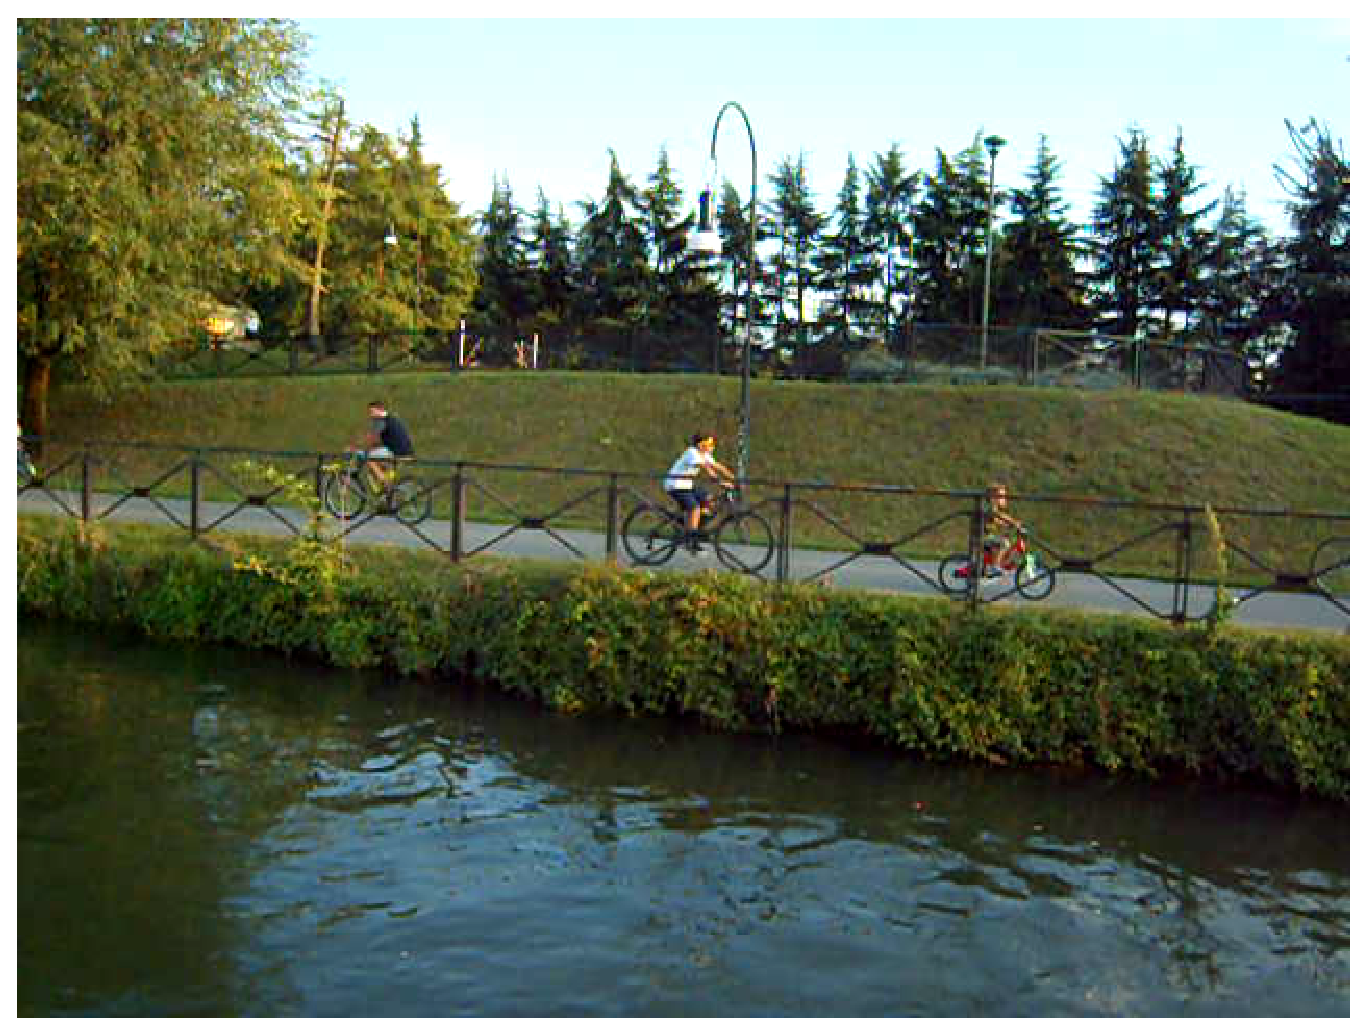
\includegraphics[width = 4cm]{./pictures/FPSalto/img0005}
	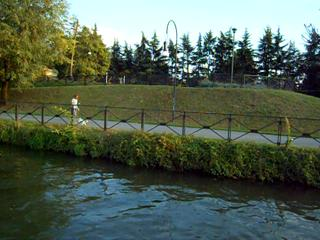
\includegraphics[width = 4cm]{./pictures/FPSalto/img0006}
	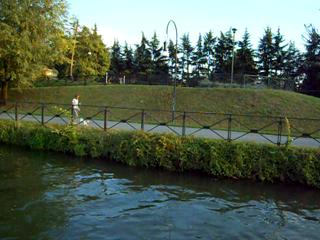
\includegraphics[width = 4cm]{./pictures/FPSalto/img0007}
	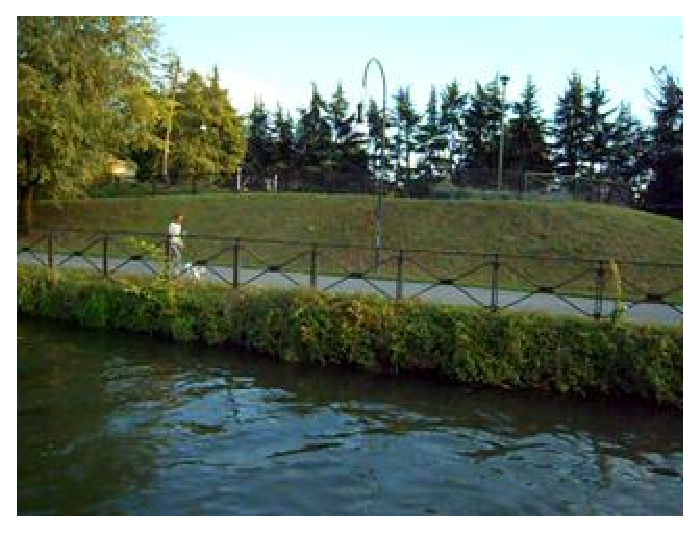
\includegraphics[width = 4cm]{./pictures/FPSalto/img0008}
	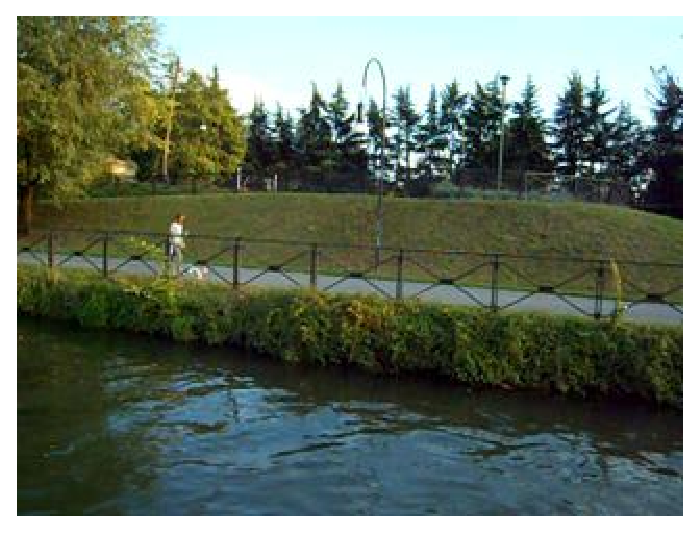
\includegraphics[width = 4cm]{./pictures/FPSalto/img0009}
	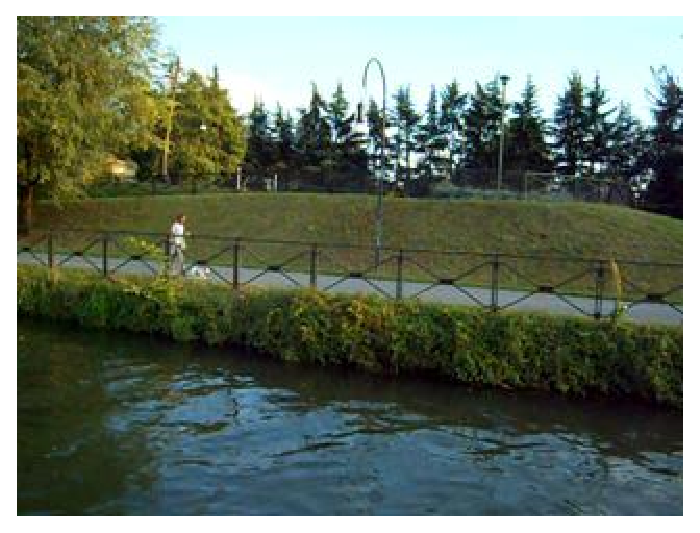
\includegraphics[width = 4cm]{./pictures/FPSalto/img0010}
	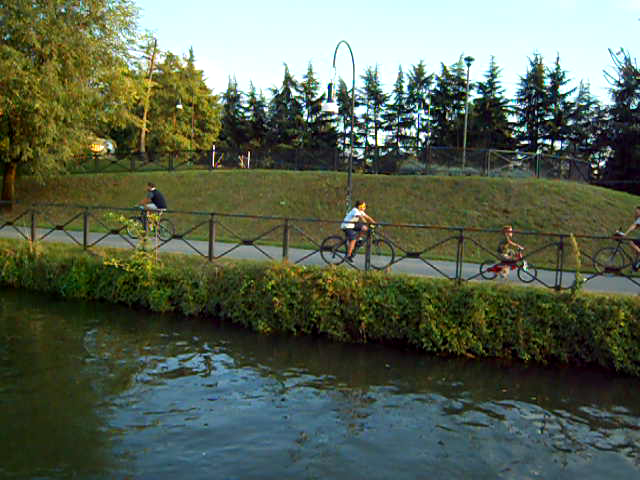
\includegraphics[width = 4cm]{./pictures/FPSalto/img0011}
	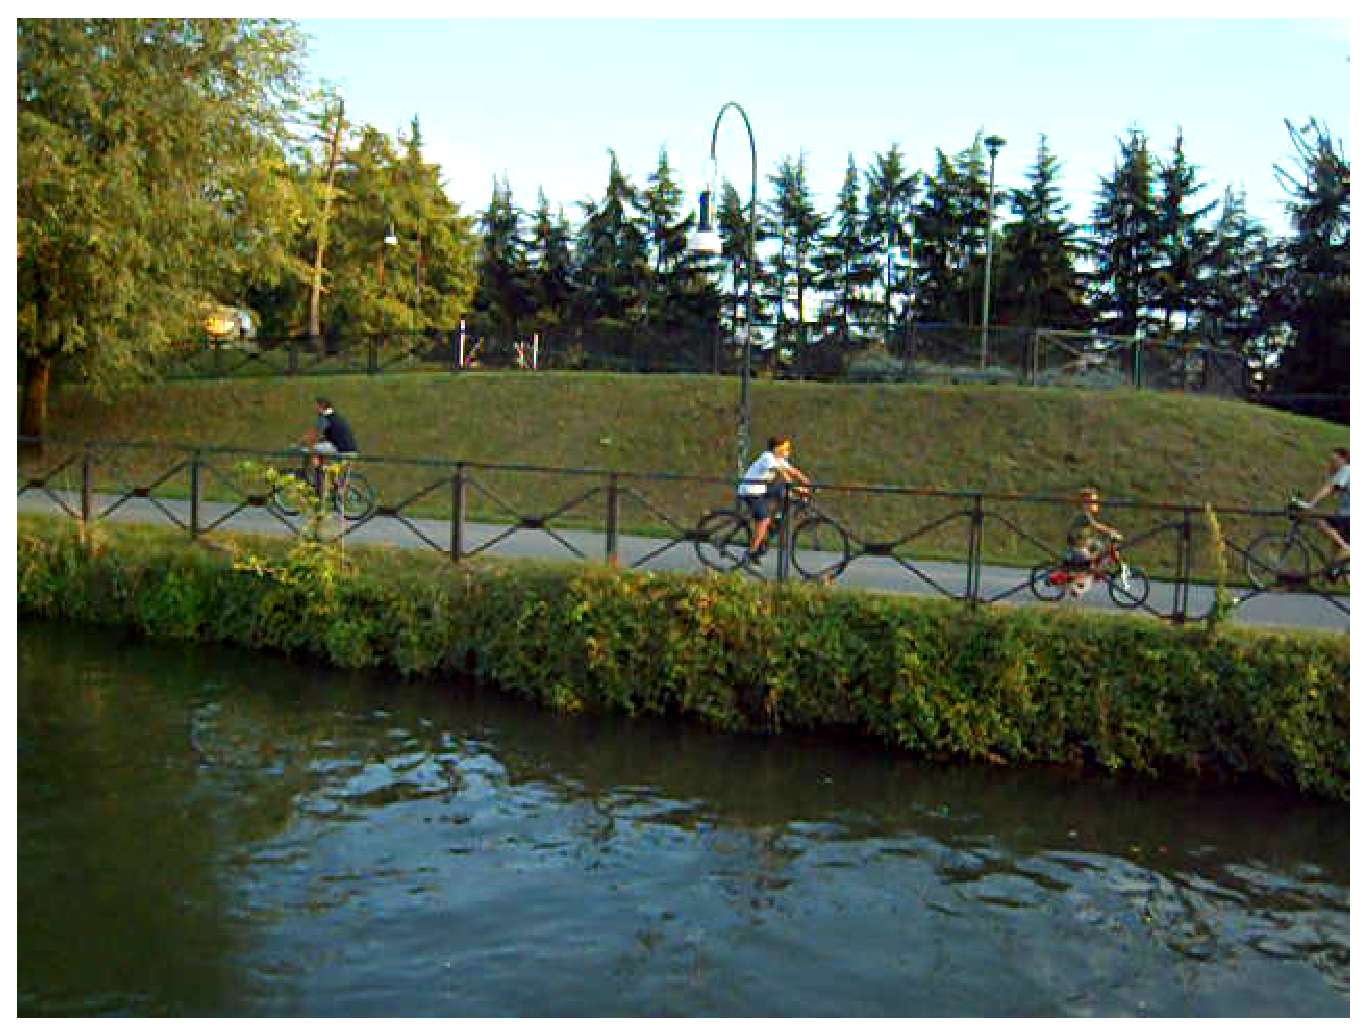
\includegraphics[width = 4cm]{./pictures/FPSalto/img0012}
	\caption{Sequenza di frame acquisiti a 30 fps}
	\label{fig:acquisizioneContinua}
\end{figure}
Un altro approccio consiste nell'analizzare la perdita di dettagli confrontando i contorni (\textit{edges}) del frame corrente con quelli del background.
Questo metodo, utilizzato in \cite{harasse2004automated}, \cite{gil2007automatic}, \cite{ellwart2012camera} e \cite{kryjak2012fpga}, consiste nell'estrarre i contorni dalle immagini secondo il metodo di Sobel \cite{sobel19683x3} o di Canny \cite{canny1986computational}, e confrontare il numero di pixel dei contorni con quelli del background. 
Quando il numero di pixel dei contorni del frame corrente $\sum edges(z_t)$ \`e $\Gamma$ volte pi\`u piccolo di quello del background $\sum edges(B_t)$:
\[ \sum edges(z_t) \leq \Gamma \sum edges(B_t), \]
dove $0<\Gamma<1$ \`e  un valore di soglia scelto in base alla sensibilit\`a che si vuole dare all'algoritmo.
\subsection{Tecniche basate su monitoraggio sequenziale}
Le tecniche viste finora, come \`e stato detto nel Paragrafo \ref{background}, permettono di aggiornare ciascun frame con un modello della scena che viene calcolato in base alle osservazioni precedenti.
\begin{figure}[tb]
	\centering
	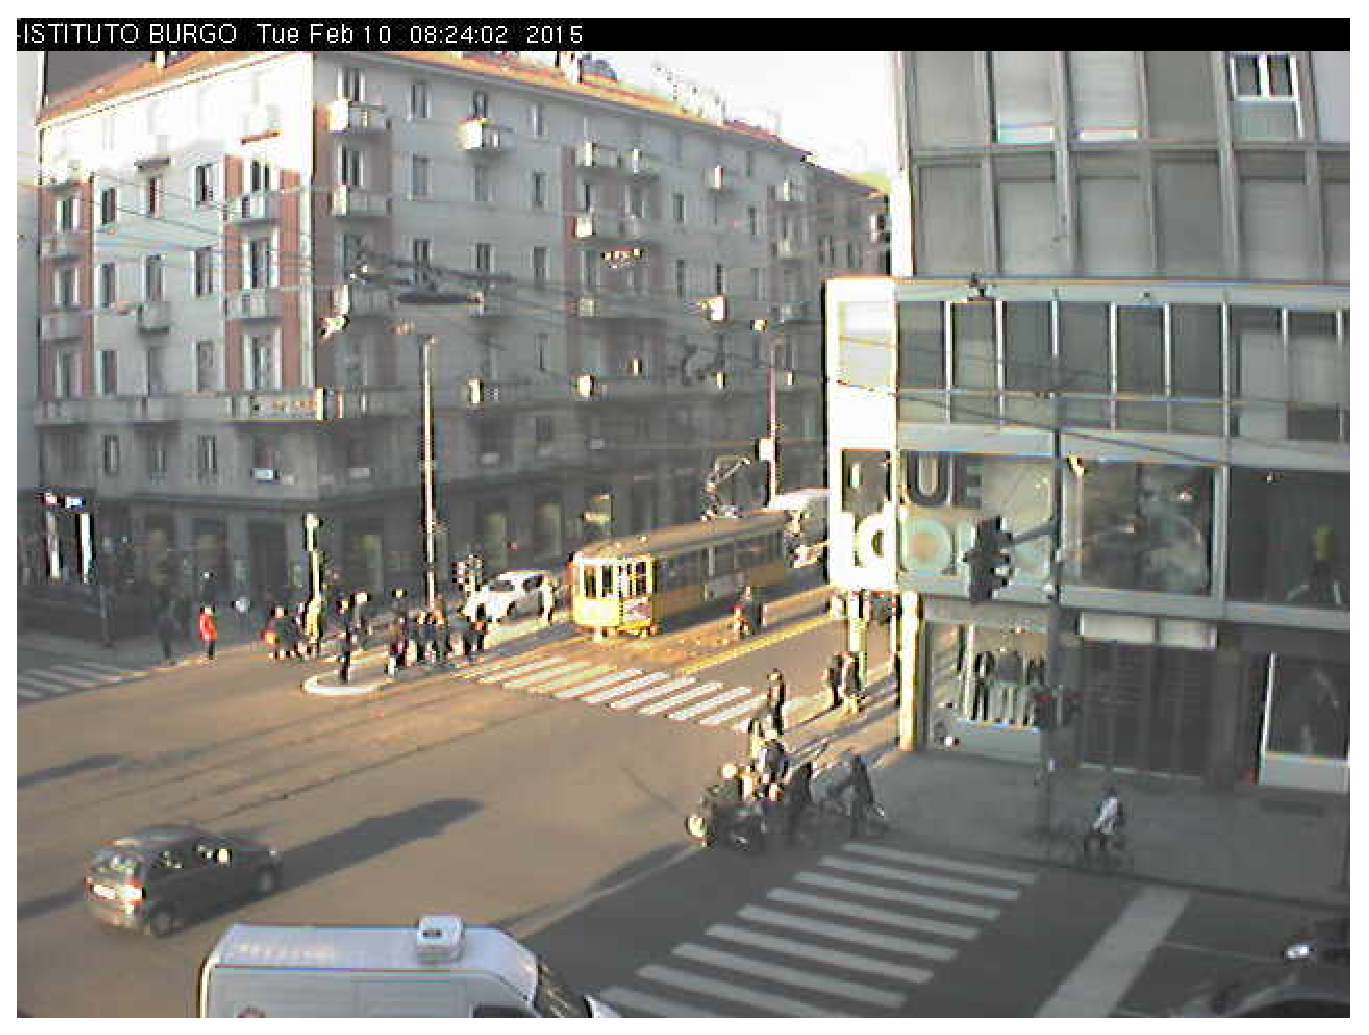
\includegraphics[width = 4cm]{./pictures/FPSbasso/image2691}
	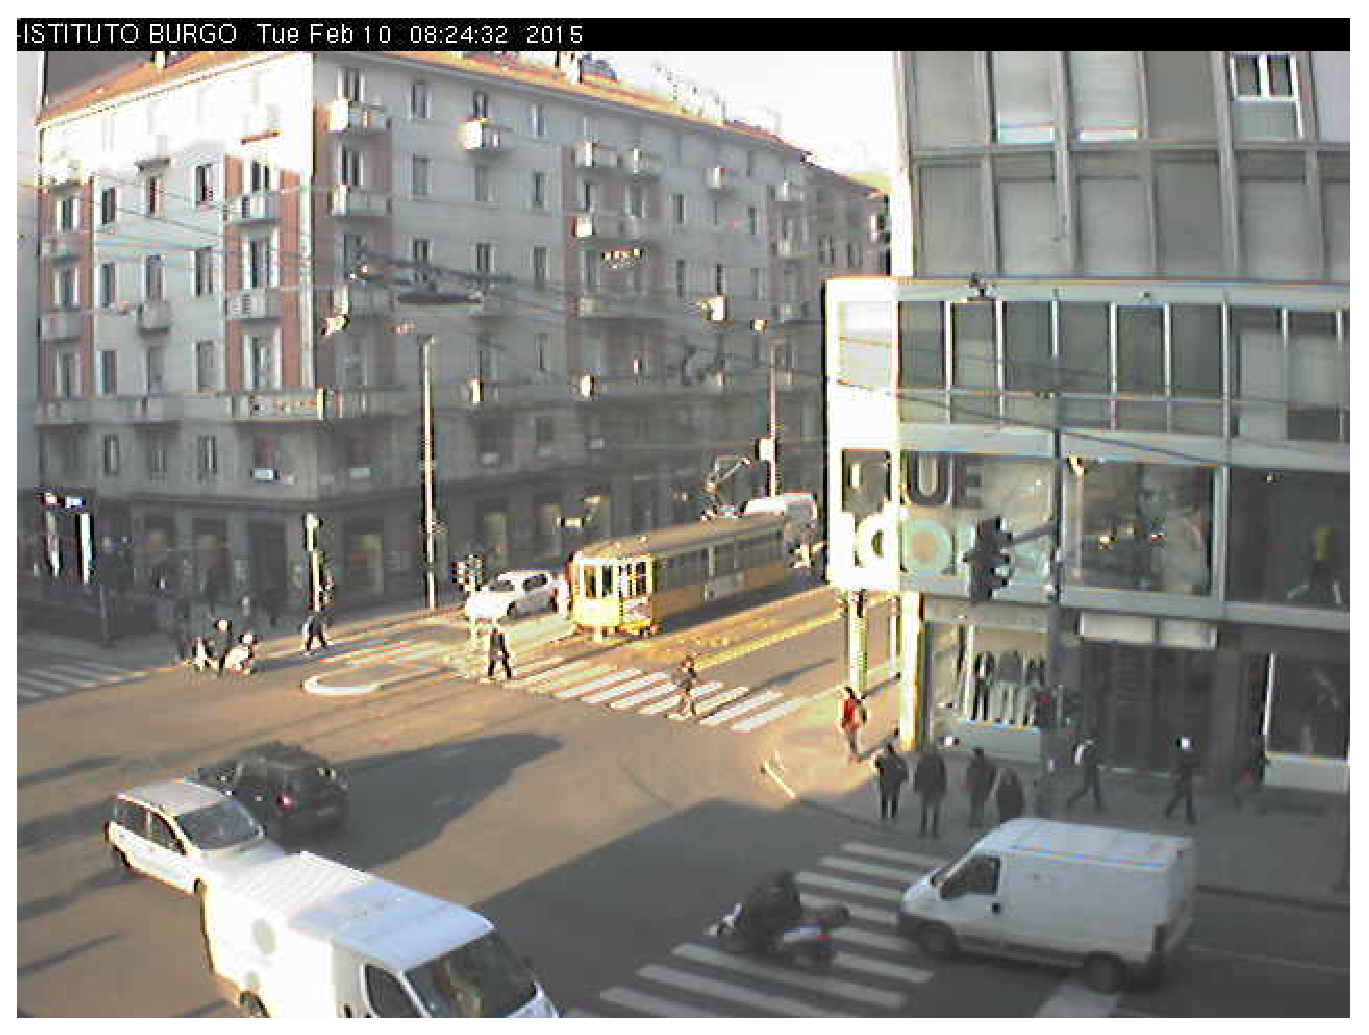
\includegraphics[width = 4cm]{./pictures/FPSbasso/image2692}
	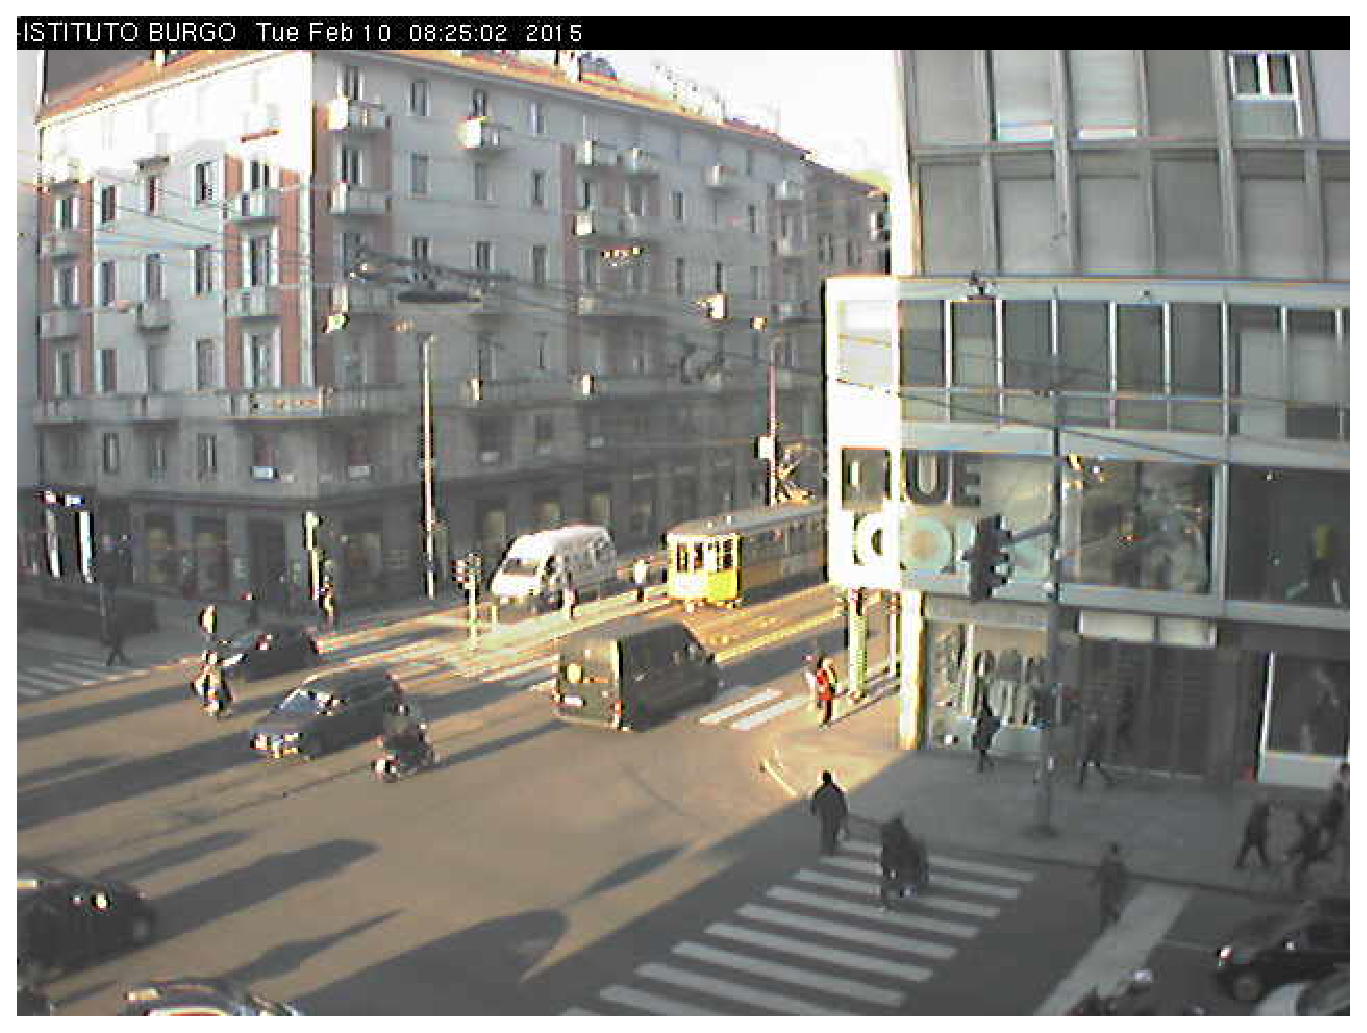
\includegraphics[width = 4cm]{./pictures/FPSbasso/image2693}
	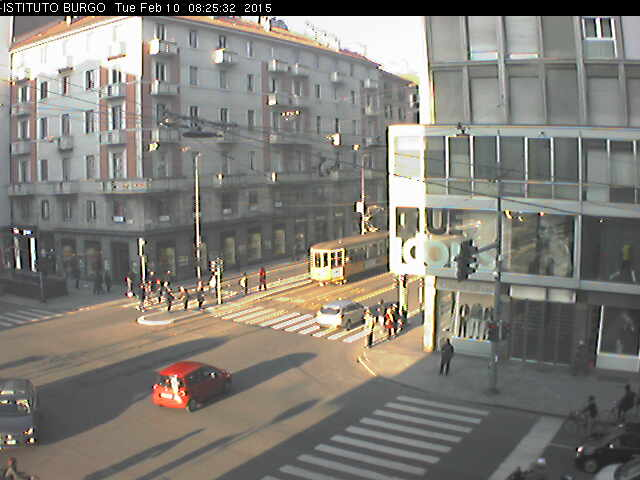
\includegraphics[width = 4cm]{./pictures/FPSbasso/image2694}
	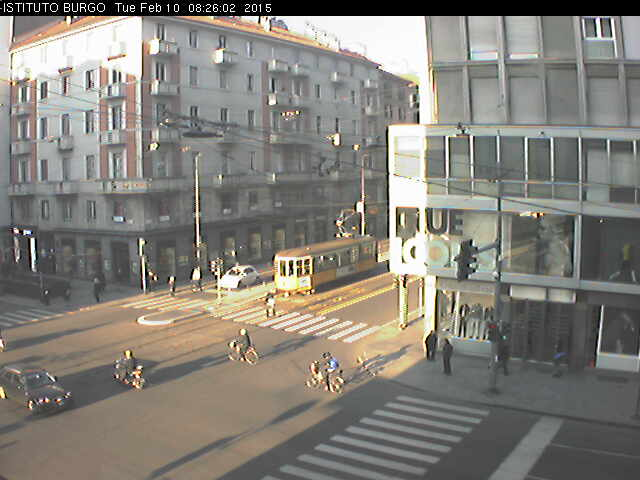
\includegraphics[width = 4cm]{./pictures/FPSbasso/image2695}
	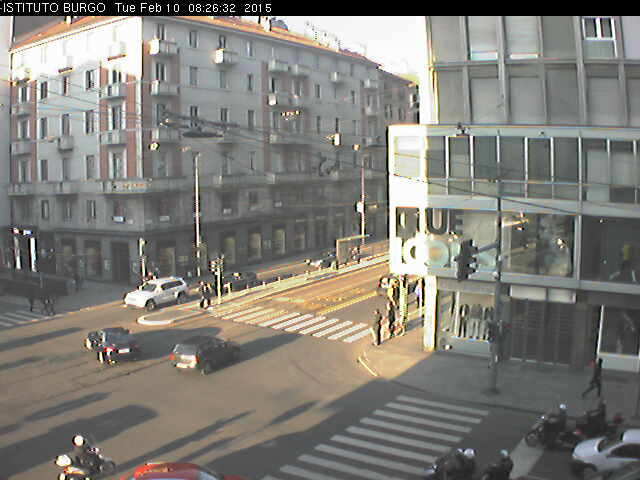
\includegraphics[width = 4cm]{./pictures/FPSbasso/image2696}
	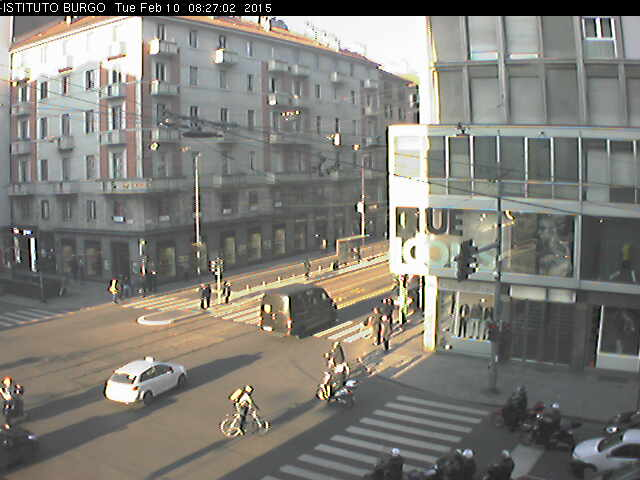
\includegraphics[width = 4cm]{./pictures/FPSbasso/image2697}
	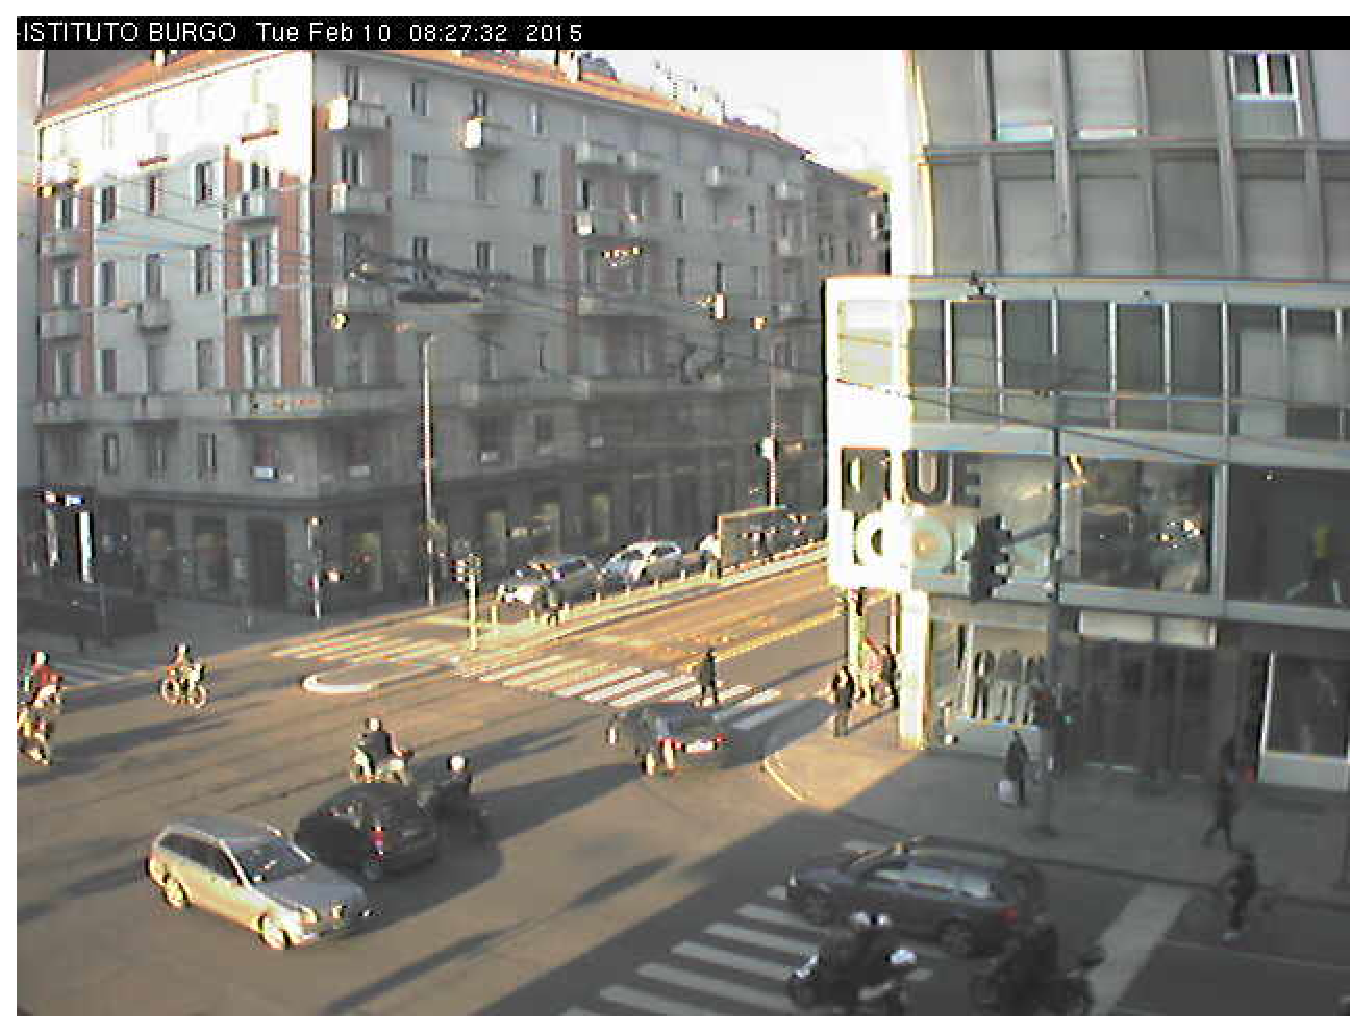
\includegraphics[width = 4cm]{./pictures/FPSbasso/image2698}
	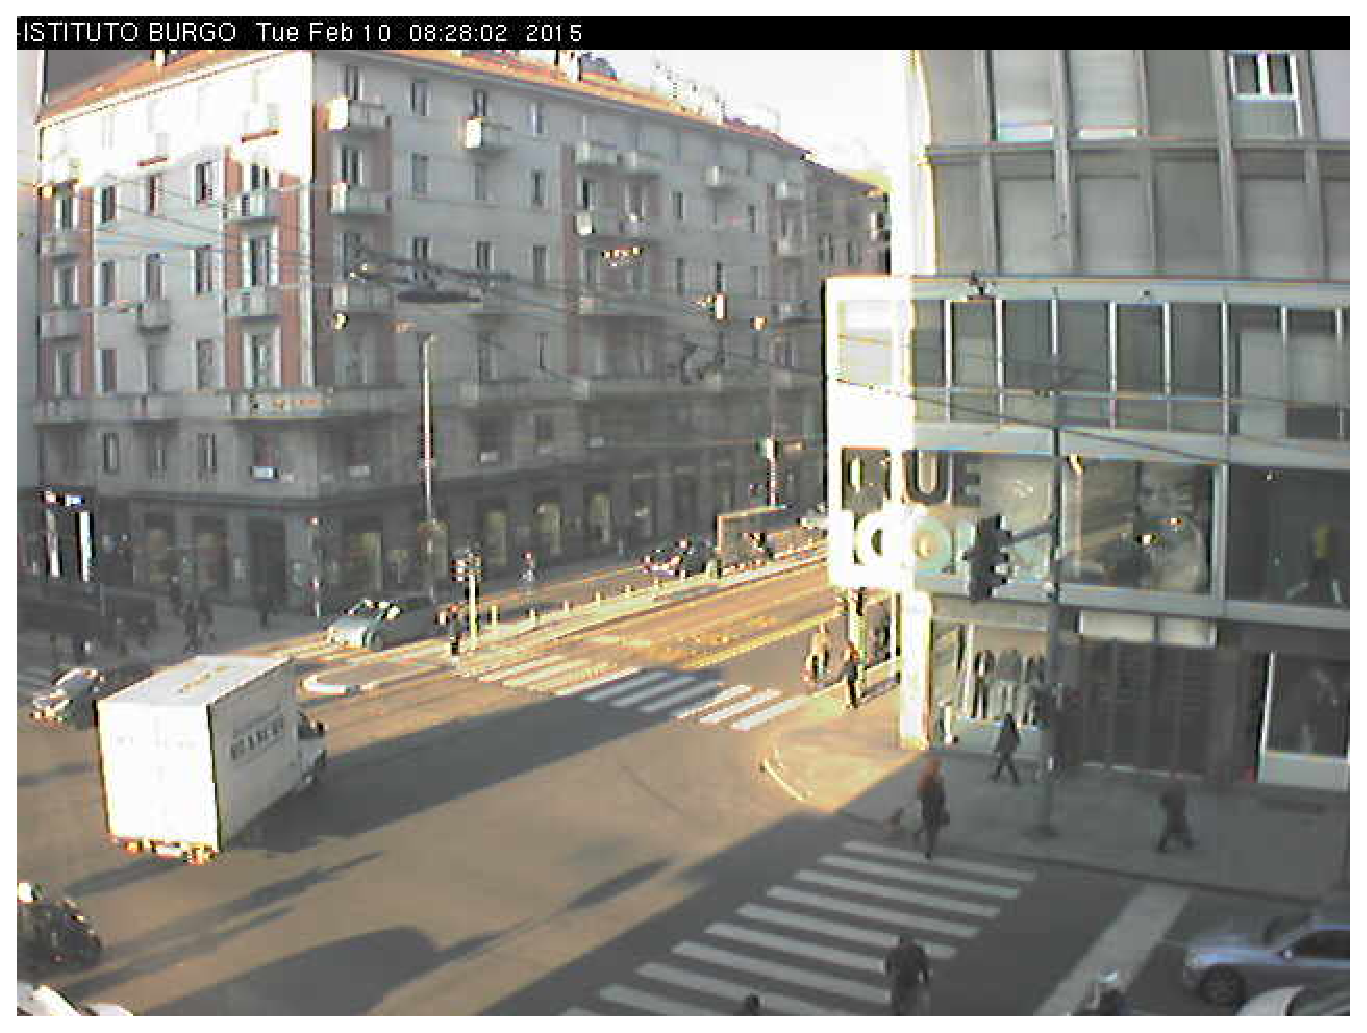
\includegraphics[width = 4cm]{./pictures/FPSbasso/image2699}
	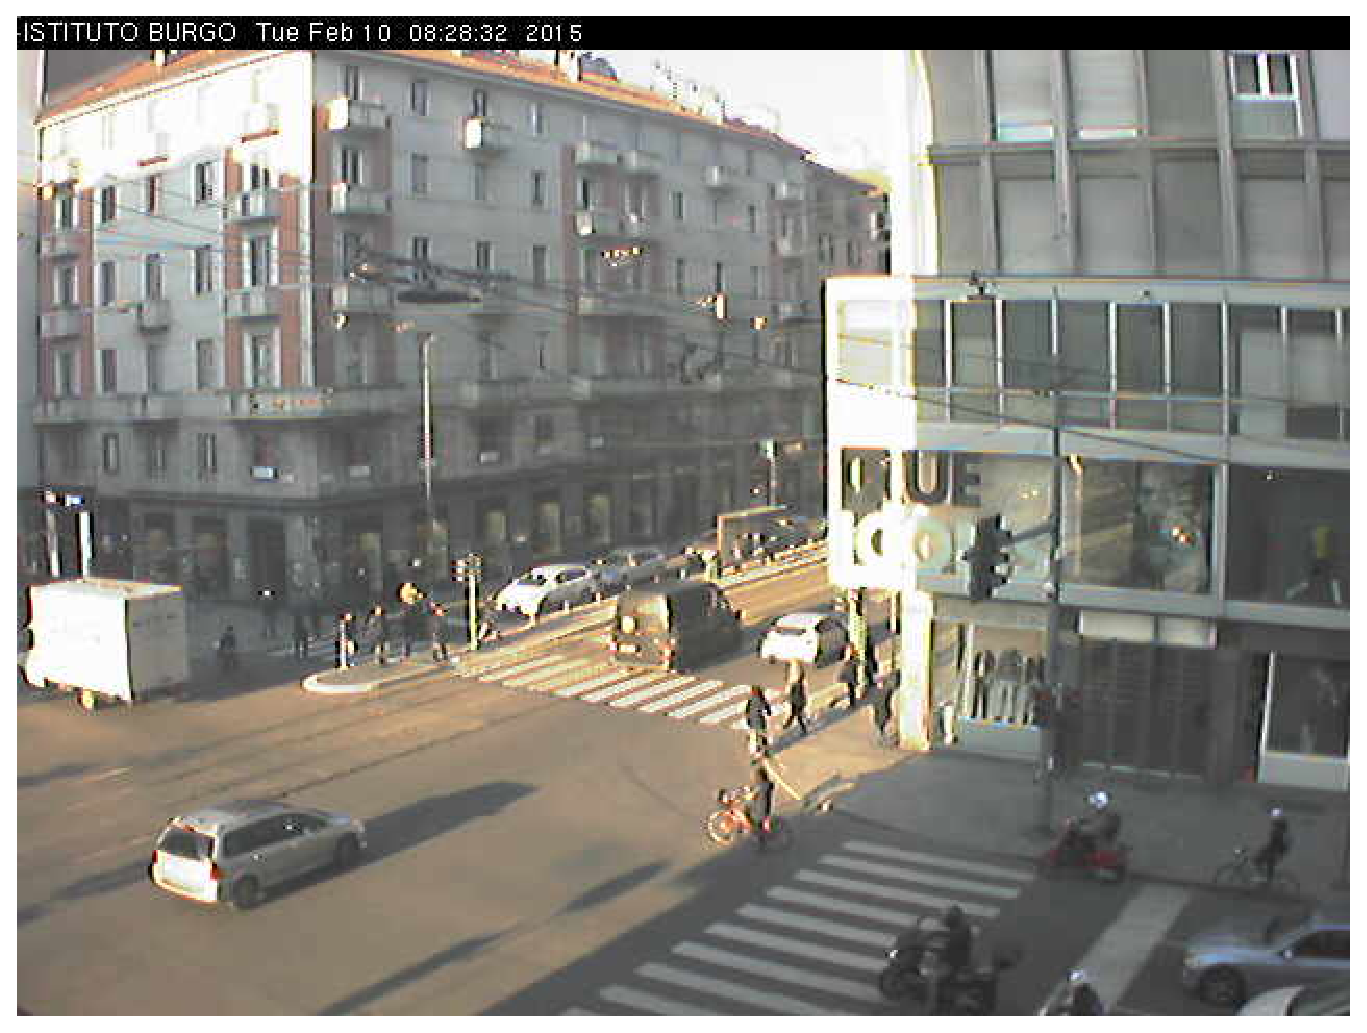
\includegraphics[width = 4cm]{./pictures/FPSbasso/image2700}
	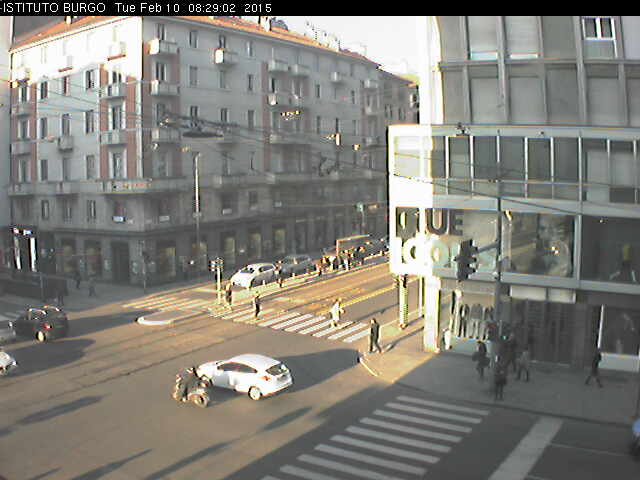
\includegraphics[width = 4cm]{./pictures/FPSbasso/image2701}
	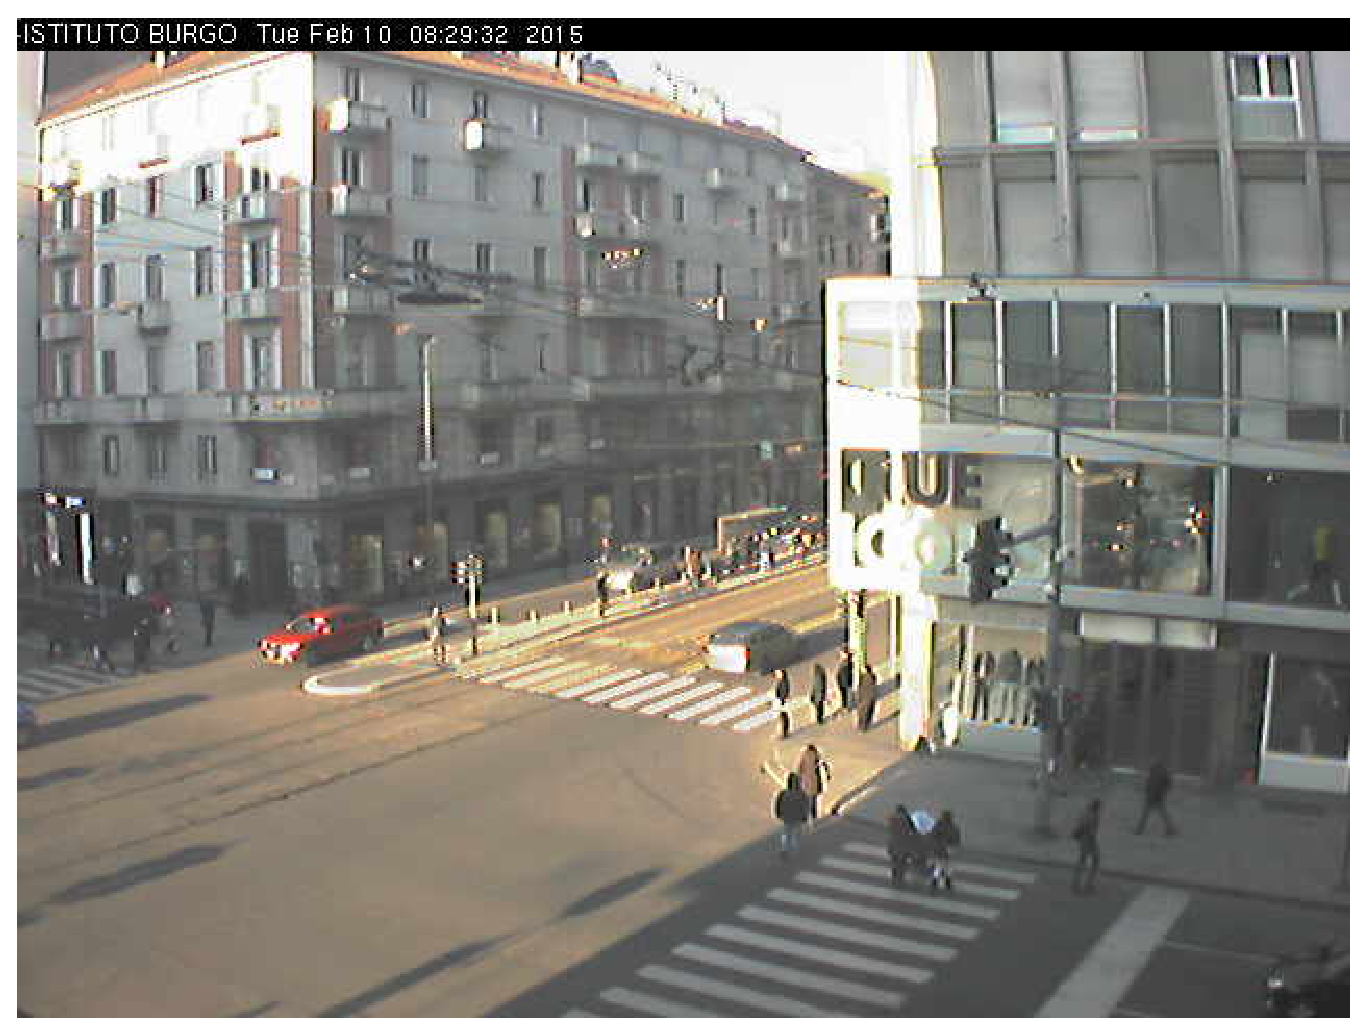
\includegraphics[width = 4cm]{./pictures/FPSbasso/image2702}
	\caption{Sequenza di frame acquisiti ogni 30 secondi}
	\label{fig:acquisizioneBassa}
\end{figure}
Questo approccio risulta fattibile nel caso in cui la camera operi con un framerate \textit{continuo}, solitamente tra i 30 frame per secondo (\textit{fps}) e i 2 fps. 
In questi casi, infatti, possiamo considerare che, tra un frame e il successivo, non avvengano grandi cambiamenti all'interno della scena e non cambi eccessivamente la luminosit\`a media.
La Figura \ref{fig:acquisizioneContinua} mostra come, in un'acquisizione fatta a 30 fps, le differenze tra frame consecutivi siano quasi inesistenti. 
Un evento di tampering pu\`o, quindi, essere identificato in maniera molto semplice, in quanto una differenza molto elevata tra il frame analizzato e il background pu\`o essere dovuto solamente a un evento di tampering sulla camera.
La Figura \ref{fig:acquisizioneBassa} mostra, invece, un esempio di frame acquisiti ogni 30 secondi.
Notiamo come le differenze tra immagini consecutive, in questo caso, siano pi\`u marcate rispetto al caso dell'acquisizione continua. 
Questo non permette l'impiego di un modello di background per il problema del tampering detection.
Evidenziamo, inoltre, che le tecniche viste finora richiedono che il sistema di monitoraggio possegga elevate capacit\`a computazionali, in quanto l'aggiornamento del background e l'analisi di tampering detection non pu\`o rallentare la frequenza di acquisizione.\\
Un approccio alternativo consiste nel monitorare nel tempo il comportamento di alcuni indicatori estratti dalle singole immagini acquisite.
Si presuppone che, quando il sistema di monitoraggio opera in condizioni di funzionamento \textit{ottimali}, gli indicatori analizzati presentino una certa \textit{stazionariet\`a}, ovvero siano considerati dei campioni \textit{indipendenti} tra loro e distribuiti secondo una stessa funzione di ripartizione.
L'evento di tampering viene considerato come un \textit{cambiamento nella stazionariet\`a} di questi indicatori.\\
Il monitoraggio pu\`o avvenire utilizzando tecniche statistiche, come ad esempio \textit{change-point method} (CPM) \cite{ross2011nonparametric} o \textit{change-detection test} \cite{pimentel2014review}.\\
Troviamo alcuni esempi nell'identificazione di sfocature: in \cite{tsesmelis2013tamper} la soluzione consiste nel monitorare nel tempo il \textit{numero di SURF} \cite{bay2006surf}, in quanto tali descrittori decrementano in maniera considerevole il loro numero in presenza di sfocature.
Notiamo, per\`o, che l'utilizzo di una tecnica del genere richiede un elevato numero di calcoli per ricavare le SURF.
Il metodo, quindi, si presta poco a essere utilizzato su sistemi di monitoraggio a basso consumo.\\
Un altro esempio \`e dato da \cite{alippi2010detecting}, dove le sfocature vengono identificate monitorando l'\textit{energia media del gradiente} delle immagini acquisite:
%\begin{equation}
%\label{eq:energyGradientSOA}
\[m_t = \mathcal{M}[z_t] = \int_{\mathcal{X}}\| \nabla z_t(x) \| _1 dx,\]
%\end{equation}  
dove $\| \cdot \|_1$ si riferisce alla \textit{norma} $\mathcal{L}_1$. 
Per identificare il cambio di stazionariet\`a di questo indicatore vengono utilizzate tecniche di CDT basate su \textit{somme cumulate} (CUSUM) \cite{alippi2008just}.\\
Il test statistico utilizzato non richiede alcuna informazione \textit{a priori} del processo che si sta monitorando, e sfrutta una sequenza iniziale $\{m_t\}, t=1,\dots,T$ di indicatori estratti da frame non sfocati, in modo da configurare automaticamente i suoi parametri. 
Tale sequenza prende il nome di \textit{training set} e, assumendo che i dati abbiano una distribuzione \textit{gaussiana,} permette di stimare i parametri di $m_t$ in assenza di sfocature che determinano l'\textit{ipotesi nulla} (indicata con $\Theta^0$), e di definire le \textit{ipotesi alternative}, indicate con $\Theta^1$, che identificano qualsiasi cambiamento non stazionario.\\
Per garantire una stima accurata dei parametri, \cite{alippi2010detecting} consiglia di utilizzare un training set ampio, ad esempio $T > 400$.
Il test opera su \textit{sotto-sequenze} di misure $m_t$ (ad esempio da $20$ misure) e stima la transizione da $\Theta^0$ a $\Theta^1$ misurando la \textit{log-verosimiglianza} tra la pdf in assenza di sfocature e le pdf delle varie ipotesi alternative nella sotto-sequenza $\tau$, ovvero
\[ r(\tau) = \ln \frac{N_{\Theta^1}(\phi_{\tau})}{N_{\Theta^0}(\phi_{\tau})}, \]
dove $\phi_{\tau}$ \`e il valore medio della misura $m_t$ nella sotto-sequenza $\tau$, e $N_{\Theta}$ \`e la \textit{distribuzione gaussiana multivariata} parametrizzata in $\Theta$.\\
Il metodo CUSUM considera la \textit{somma cumulata} 
\[ S(\tau) = \sum^\tau_{t=1} r(t) \]
e identifica un cambiamento in $m_t$ quando \[g(\tau)=S(\tau)-\nu(\tau),\] ovvero la differenza tra il valore della somma cumulata all'istante $\tau$ e il suo valore minimo nel tempo \[\nu(\tau)=\min_{t=1,...,\tau}S(t),\] supera una certa soglia $h$.\\
L'utilizzo di un descrittore leggero come l'energia media del gradiente permette di operare con una bassa complessit\`a computazionale, tanto da poter essere utilizzato come soluzione a livello di nodo per una \textit{wireless multimedia sensor network} (WMSN) \cite{akyildiz2007survey}.
D'altro canto, confrontato con le tecniche descritte nel Paragrafo \ref{background}, l'utilizzo di tecniche sequenziali genera un numero pi\`u alto di \textit{falsi allarmi}, il che si traduce, all'interno di una rete di sensori, in un aumento dei messaggi di allarme inviati, che devono essere considerati, quindi, come un costo.













\chapter{Impostazione del problema di ricerca}
\label{FormulazioneProblema}
\thispagestyle{empty}

%\begin{quotation}
%{\footnotesize
%\noindent{\emph{``Terence: Rotta a nord con circospezione \\
%Bud: Ehi, gli ordini li do io qui!\\
%Terence: Ok, comante\\
%Bud: Rotta a nord\\
%Terence: Soltanto?\\
%Bud: Con circospezione!''}
%}
%\begin{flushright}
%Chi Trova un Amico Trova un Tesoro
%\end{flushright}
%}
%\end{quotation}
\vspace{0.5cm}
In questo capitolo descriviamo il problema affrontato dall'algoritmo di tampering detection, in maniera formale e rigorosa. Il primo paragrafo illustra il modello delle osservazioni e gli eventi che siamo interessati a identificare, mentre il secondo paragrafo formalizza il concetto di tampering detection. 
\noindent 
\section{Modello delle osservazioni}
\label{modelloOsservaz}
Il nostro campo di osservazione si concentra su quegli eventi che si interpongono tra la scena ripresa da una camera e il sensore che acquisisce le immagini. Non vogliamo, cio\`e, identificare degli eventi particolari che avvengono nella scena, come un oggetto lasciato incustodito \cite{Targhe}, bens\`i vogliamo identificare quegli eventi che non permettano al sensore di riprendere in maniera ottimale la scena, quali ad esempio sfocature o spostamenti della camera.
Nel seguito cerchiamo di dare una definizione formale di questi eventi.
\subsection{Sfocatura}
\label{sfocatura}
Il fenomeno della sfocatura avviene quando un elemento trasparente o semitrasparente si interpone tra la lente della camera e la \gls{scena} ripresa, oppure quando viene cambiata la messa a fuoco, causando una perdita nei dettagli della \gls{scena} ripresa.

\begin{figure}
	\centering
	\begin{subfigure}[]
		{\label{fig:pioggia} 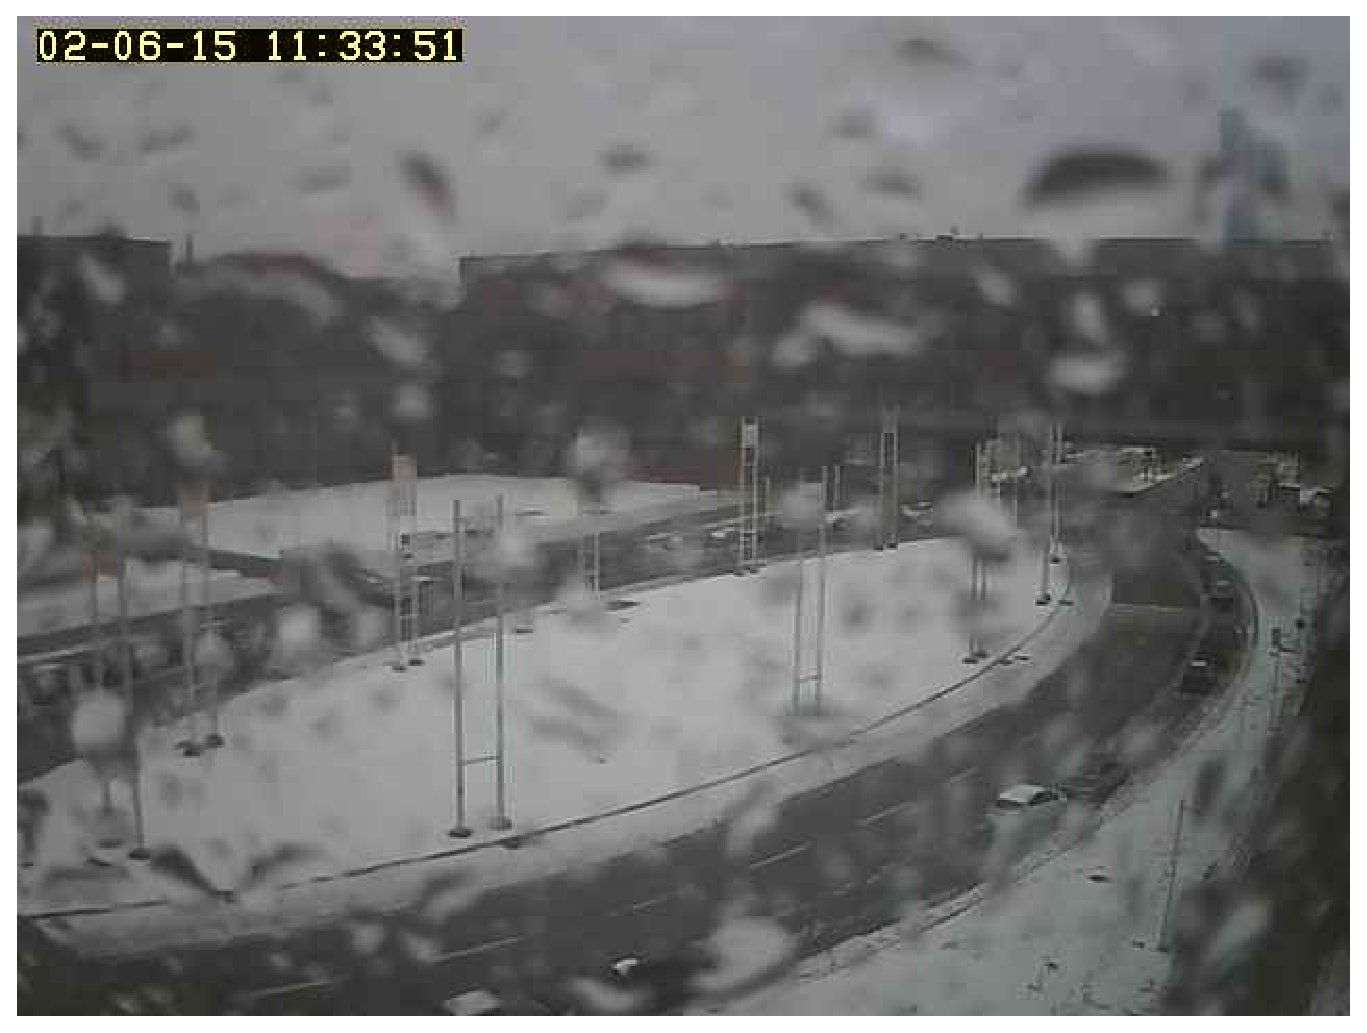
\includegraphics[width=6cm]{./pictures/pioggia}}
	\end{subfigure}
	\begin{subfigure}[]
		{\label{fig:bassiniDEFOCUS} \includegraphics[width=6cm]{./pictures/bassiniDEFOCUS}}
	\end{subfigure}
	\caption{Esempi di sfocature}
	\label{fig:esempiSfocature}
\end{figure}
\noindent Nella figura \ref{fig:esempiSfocature} sono mostrati degli esempi in cui sono presenti delle sfocature. 
Queste possono essere di origine diversa: 
\begin{itemize}
	\item dovute a \textit{cause naturali}, come ad esempio dell'acqua piovana che si deposita sulla lente (figura \ref{fig:pioggia}), o la condensa dovuta all'umidit\`a e alle basse temperature, oppure un raggio di sole incidente sull'obiettivo della camera;
	\item per \textit{intervento dell'uomo}, che a sua volta pu\`o avvenire in maniera intenzionale (e in questo caso si pu\`o parlare di \textit{manomissione}) oppure non intenzionale. Ad esempio, si pu\`o direttamente intervenire sulla messa a fuoco, nel caso sia possibile cambiarla manualmente; oppure (come nel caso della figura \ref{fig:bassiniDEFOCUS}) \`e possibile applicare una sostanza semitrasparente sulla lente della camera, come il gas di un deodorante spray.
\end{itemize}
Inoltre, possiamo notare come nella figura \ref{fig:bassiniDEFOCUS} la sfocatura riguardi tutta l'immagine, mentre nella figura \ref{fig:pioggia} la sfocatura si concentri solo in alcune aree (quelle dove sono presenti le gocce). 
Nel primo caso si parler\`a, quindi, di sfocatura \textit{totale}, mentre nel secondo caso di sfocatura \textit{parziale}.\\
Riprendendo la trattazione presente in \cite{alippi2010detecting}, questo fenomeno pu\`o essere modellato come un operatore di \textit{degradazione} $\mathcal{D}$ applicato a un'immagine $y$, considerata priva di errori, i.e.,
\begin{equation}
z=\mathcal{D}[y].
\end{equation}
In particolare, all'interno dell'operatore $\mathcal{D}$ si pu\`o considerare il contributo dovuto a un operatore di \textit{sfocatura} $\mathcal{B}$ (dall'inglese \textit{blur}) e un termine aleatorio $\eta$ corrispondente al rumore, i.e.,
\begin{equation}
\label{blur_single}
z(x)=\mathcal{D}[y](x) = \mathcal{B}[y](x) + \eta(x), \qquad x \in \mathcal{X}
\end{equation}
dove, come abbiamo specificato nel paragrafo \ref{concetti}, indichiamo con $x$ le coordinate dei \textit{pixel} dell'immagine e con $\mathcal{X}$ l'insieme dei pixel che formano l'immagine. 
Per praticit\`a possiamo assumere che l'operatore di blur sia \textit{lineare}.
Quindi, considerando l'immagine come un dato \textit{continuo},
\begin{equation}
\label{eq:blur}
\mathcal{B}[y](x) = \int_{\mathcal{X}}y(s)h(x,s)ds,
\end{equation}
dove $h(x,\cdot)$ rappresenta la \textit{risposta all'impulso}, \textit{point spread function} (PSF), della sfocatura sul pixel $x$.
L'effetto di $h(x, \cdot)$ \`e quello di rendere le differenze di intensit\`a, tra pixel adiacenti, pi\`u morbide (\textit{smooth}).
Nel caso in cui la sfocatura sia applicata sulla totalit\`a dell'immagine e fosse \textit{spazio invariante} (come nel caso della figura \ref{fig:bassiniDEFOCUS}), allora \`e possibile modellare l'operatore di blur come una \textit{convoluzione}\footnote{Il blur convoluzionale \`e quello che abbiamo utilizzato per generare, in maniera sintetica, sequenze con immagini sfocate.}:
\begin{equation}
\label{blur_convolution}
\mathcal{B}[y](x) = \int_{\mathcal{X}}y(s)h(s-x)ds,
\end{equation}
dove $h(\cdot)$ \`e un filtro gaussiano o uniforme.\\
Nel caso pi\`u generale possiamo considerare che la camera acquisisca una sequenza di $N$ osservazioni $\{z_i\}, i = 1, \dots ,N$, quindi la formula \eqref{blur_single} si pu\`o riscrivere come
\begin{equation}
\label{blur_multi}
z_i(x)=\mathcal{D}_i[y_i](x) = \mathcal{B}_i[y_i](x) + \eta(x), \qquad x \in \mathcal{X}.
\end{equation}
La sequenza delle immagini $\{y_i\}, i = 1,\dots , N$, pu\`o variare in maniera significativa nel suo contenuto, anche nel caso in cui la vista sia la stessa.
\begin{figure}
	\centering
	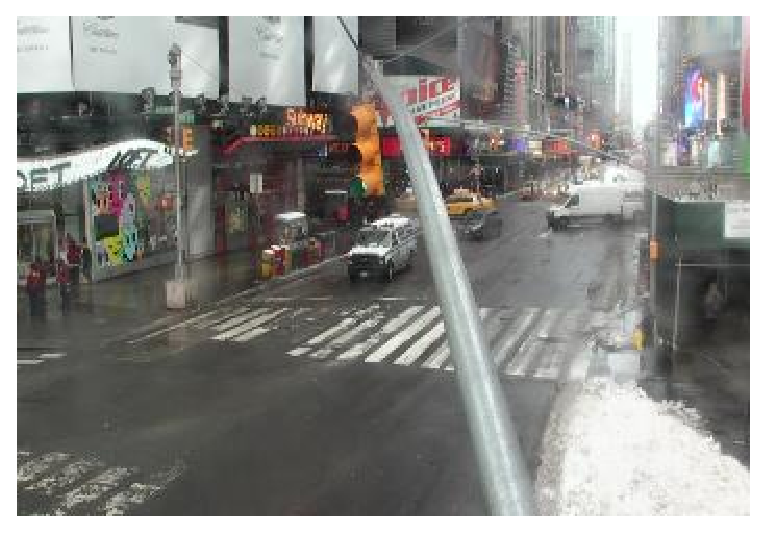
\includegraphics[width=3cm]{./pictures/image0001.eps}
	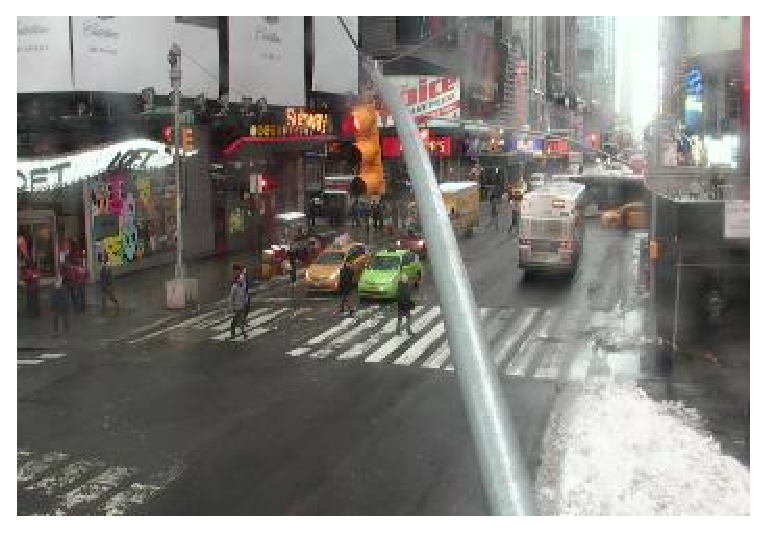
\includegraphics[width=3cm]{./pictures/image0002.eps}
	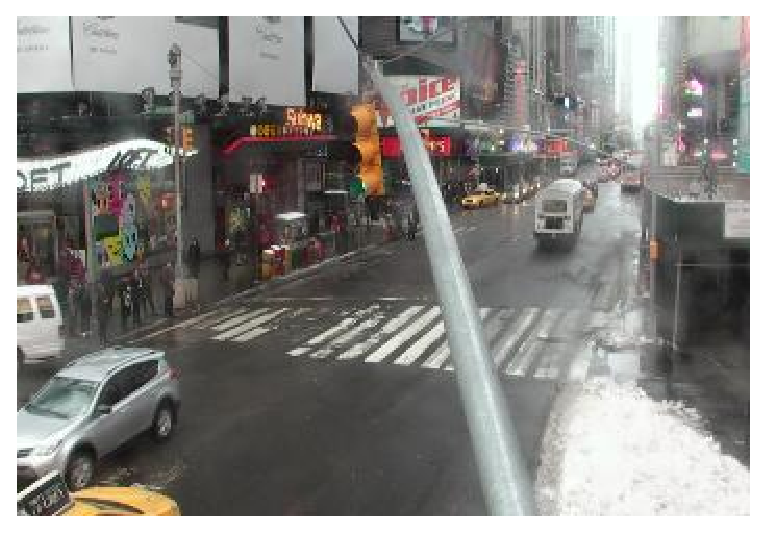
\includegraphics[width=3cm]{./pictures/image0003.eps}
	\includegraphics[width=3cm]{./pictures/image0004.eps}
	\includegraphics[width=3cm]{./pictures/image0005.eps}
	\includegraphics[width=3cm]{./pictures/image0006.eps}
	\includegraphics[width=3cm]{./pictures/image0007.eps}
	\includegraphics[width=3cm]{./pictures/image0008.eps}
	\caption{Sequenza di otto frame consecutivi acquisiti ogni minuto}
	\label{fig:framDifferences}
\end{figure}
\noindent Un esempio \`e illustrato nella figura \ref{fig:framDifferences}, in cui le immagini riprese dalla camera sono acquisite ogni minuto. 
Nonostante l'inquadratura non cambi tra le acquisizioni, il contenuto delle singole immagini varia parecchio, a causa del continuo passaggio di automobili e pedoni.
Questo problema fa s\`i che l'identificazione delle sfocature non possa avvenire facendo un semplice confronto tra frame consecutivi, in quanto avremmo un numero troppo elevato di falsi positivi.
Infatti, nel caso in cui avessimo un riscontro negativo dal confronto tra due frame ($z_i \neq z_{i + 1}$), sarebbe difficile capire se \`e cambiato il contenuto delle immagini ($y_i \neq y_{i + 1}$) o l'operatore di sfocatura ($\mathcal{B}_i \neq \mathcal{B}_{i + 1}$). 
\subsection{Spostamento della camera}
\label{displacement}
Lo spostamento della camera avviene quando cambia la sua inquadratura.
Le cause possono essere, ancora una volta, di tipo naturale, ad esempio una raffica di vento che sposta la camera, oppure dovute a un intervento umano, uno spostamento intenzionale per evitare che la scena venga ripresa.
\begin{figure}
	\centering
	\subfigure[]{\label{fig:displacementORIGINALE} \includegraphics[width=6cm]{./pictures/testiORIGINALE}}
	\subfigure[]{\label{fig:displacementSPOSTATO}\includegraphics[width=6cm]{./pictures/testiDISPLACEMENT}}
	\caption{Esempio di spostamento della camera}
	\label{fig:testiDISPLACEMENT}
\end{figure}
\noindent Un esempio \`e mostrato nella figura \ref{fig:testiDISPLACEMENT}, dove vediamo che tra il frame riportato in figura \ref{fig:displacementORIGINALE} e quello in figura \ref{fig:displacementSPOSTATO} c'\`e stato un evento che ha spostato la camera.
Possiamo formalizzare il concetto di spostamento della camera nel modo seguente: consideriamo la sequenza $\{y_i\}$ di immagini generate da una camera in una certa posizione, e la sequenza $\{w_i\}$ di immagini generate dalla stessa camera in una posizione differente.\\
Possiamo modellare la sequenza di immagini $\{z_i\}$ in cui avviene uno spostamento della camera all'istante $T^*$ nel seguente modo:
\begin{equation}
\label{eq:displacement}
z_i(x)  = \left\{ \begin{array}{rcl}
	y_i(x) + \eta(x) & \mbox{per} & i < T^* \\
	w_i(x) + \eta(x) & \mbox{per} & i \geqslant T^*
	\end{array}\right. ,
\end{equation}
dove $\eta(x)$ \`e un rumore stazionario.\\
In questa formulazione abbiamo considerato lo spostamento come un fenomeno \textit{istantaneo};
in generale, possiamo considerare una fase \textit{transitoria} in cui l'inquadratura della camera cambia a ogni \gls{frame} acquisito, fino a raggiungere la posizione finale. 
Dato che, nella nostra applicazione, la camera opera con \gls{framerate} molto bassi (come ad esempio un'immagine al minuto), possiamo considerare lo spostamento come istantaneo e, quindi, tenere come riferimento il modello \eqref{eq:displacement}.\\
%Nella formulazione pi\`u generale possiamo, quindi, assumere un istante $T_{start}^ *$ in cui inizia lo spostamento e un istante $T_{end}^*$ in cui termina il transitorio:
%\begin{equation}
%\label{eq:displacementGeneral}
%z_i(x) = \left\{ \begin{array}{rcl}
%y_i(x) + \eta(x) & \mbox{per} & i < T_{start}^* \\
%v_i(x) + \eta(x) & \mbox{per} & T_{start}^* \leq i < T_{end}^* \\
%w_i(x) + \eta(x) & \mbox{per} & i \geqslant T_{end}^*
%\end{array}\right. ,
%\end{equation}
%dove $\{v_i\}$ rappresenta la sequenza di immagini generate da viste differenti.
%Inoltre, durante il transitorio dello spostamento, il tempo di esposizione della camera pu\`o portare alla generazione di sfocature nelle immagini.\\
Anche per lo spostamento della camera vale la considerazione fatta nel caso della sfocatura: il contenuto delle immagini varia con il passare del tempo, quindi identificare lo spostamento confrontando frame consecutivi nel tempo genera un alto numero di falsi allarmi, come verr\`a mostrato dalla fase sperimentale.
\subsection{Occlusione e guasti della camera}
Il fenomeno dell'occlusione avviene quando un oggetto opaco si pone a ridosso della camera, impedendo la visione di una parte, se non la totalit\`a, della scena. 
\begin{figure}
	\centering
	\subfigure[]{\label{fig:occlusionCALZA} \includegraphics[width=6cm]{./pictures/calza}}
	\subfigure[]{\label{fig:occlusionNEVE}\includegraphics[width=6cm]{./pictures/neve}}
	\caption{Esempi di occlusione}
	\label{fig:occlusion}
\end{figure}
\noindent Esempi di occlusione sono illustrati in figura \ref{fig:occlusion}. 
Pu\`o succedere (Fig. \ref{fig:occlusionCALZA}) che un oggetto venga posto intenzionalmente davanti alla lente della camera, in modo da coprire la scena, oppure (Fig. \ref{fig:occlusionNEVE}), a causa di una nevicata, pu\`o avvenire che della neve si depositi sulla lente e, quindi, venga compromessa la corretta acquisizione.\\
Quando parliamo di guasti, invece, possiamo considerare due casi:
\begin{itemize}
	\item guasto della \textit{trasmissione};
	\item guasto del \textit{sensore.}
\end{itemize}
Il primo caso pu\`o avvenire quando considerano delle WMSN, in particolare quando i frame vengono trasmessi attraverso la rete dai sensori verso un nodo centrale.
Quando avviene un guasto nella rete parte dell'immagine non viene trasmessa, come illustrato nella figura \ref{fig:guastoTrasmissione}.
Il caso del sensore guasto, come ad esempio quello nella figura \ref{fig:guastoSensore}, comporta generalmente un aumento del rumore presente nel frame. \\
\begin{figure}
	\centering
	\subfigure[]{\label{fig:guastoTrasmissione} \includegraphics[width=6cm]{./pictures/erroreTrasm}}
	\subfigure[]{\label{fig:guastoSensore}\includegraphics[width=6cm]{./pictures/rumore}}
	\caption{Esempi di guasti}
	\label{fig:guasti}
\end{figure}
Questi problemi non sono stati affrontati durante il corso della tesi, comunque le tecniche messe a punto per rilevare spostamenti e sfocature possono essere utilizzate anche per rilevare questo tipo di eventi. 
\section{Tampering detection}
Nel paragrafo \ref{tamperingSOA} abbiamo introdotto in maniera molto generale il concetto di tampering detection. 
In questo paragrafo diamo una definizione pi\`u formale al problema.
L'algoritmo di tampering detection consiste nell'analizzare la sequenza dei frame generati dalla camera in modo da determinare un possibile cambiamento nell'inquadratura della scena o una sfocatura.\\
Consideriamo il caso generale di una sequenza di frame $\{z_i\}, i=1,\dots,\infty$. 
Per $i<T^*$ abbiamo che i frame vengono acquisiti in condizioni di funzionamento normale:
\[ z_i(x)=y_i(x) + \eta(x), \forall x \in \mathcal{X} \mbox{, per } i=1,\dots , T^*-1. \] 
All'istante di tempo $i = T^*$ avviene un evento di tampering, il quale compromette i frame per $i\geq T^*$.  
In particolare, nel caso di una sfocatura avremo
\[ z_i = B_i[y_i](x) + \eta(x), \forall x \in \mathcal{X} \mbox{, per } i \geq T^*,\]
mentre nel caso di uno spostamento della camera avremo
\[ z_i = w_i(x) + \eta(x), \forall x \in \mathcal{X} \mbox{, per } i \geq T^*. \]
%Nel caso dell'operatore di degradazione $\mathcal{D}$, con riferimento al modello descritto nell'equazione \eqref{blur_multi}, possiamo considerare che, in condizioni di funzionamento normale, l'operatore di sfocatura $\mathcal{B}$ si comporti come un \textit{filtro passa-tutto}, ovvero
%\[\mathcal{B}_i[y](x)=y_i(x) \mbox{, per } i=1,\dots, T^*,\]
%e che all'istante $T^*$ esso cambi, diventando come nel caso dell'equazione \eqref{eq:blur}.
L'obiettivo dell'algoritmo \`e quello di stimare l'istante $T^*$. \\
%Nel caso dell'operatore di spostamento $\mathcal{S}$, tenendo come riferimento la formula \eqref{eq:displacement}, l'obiettivo dell'algoritmo \`e quello di stimare l'istante di tempo $T^*$ in cui avviene il passaggio dalla sequenza di immagini $\{y_i\}$ a $\{w_i\}$.\\
Come abbiamo illustrato precedentemente, discriminare tra cambiamenti avvenuti a livello di contenuto della scena e cambiamenti dovuti a tampering pu\`o diventare complicato confrontando direttamente i frame tra loro, in quanto stiamo operando con framerate bassi.
%Non \`e, quindi, possibile utilizzare le tecniche basate su background che sono state descritte nel paragrafo \ref{background}.
Non utilizzeremo, quindi, le tecniche basate su background che sono state descritte nel paragrafo \ref{background}.
Nel prossimo capitolo vedremo la soluzione che abbiamo deciso di utilizzare per lo sviluppo dell'algoritmo di tampering detection. 
\chapter{Soluzione proposta}
\label{SoluzioneProposta}
\thispagestyle{empty}

%\vspace{0.5cm}

\noindent In questo capitolo descriviamo la soluzione che abbiamo proposto per risolvere il problema del tampering detection, formulato nel Capitolo \ref{FormulazioneProblema}.\\
Nel Paragrafo \ref{indicatori} descriviamo quali sono gli indicatori che abbiamo deciso di monitorare per individuare gli eventi di tampering.\\
Nel Paragrafo  \ref{monitoraggio} illustriamo in che modo vengono monitorati questi indicatori in modo da individuare degli eventi specifici.\\
Nel Paragrafo \ref{segmentazione} descriviamo, infine, l'algoritmo di segmentazione che utilizziamo, assieme al monitoraggio, per individuare eventi di spostamento della camera.
\section{Indicatori utilizzati per identificare gli eventi di tampering}
\label{indicatori}
L'approccio che abbiamo considerato per risolvere il problema del tampering detection consiste nell'estrarre, da ciascun frame ripreso dalla camera, degli indicatori \textit{scalari} che possano essere monitorati nel tempo, in modo da individuare un cambio di distribuzione o un \textit{outlier} associabile a un evento di tampering. 
In particolare abbiamo deciso di considerare un indicatore in grado di verificare la presenza di sfocature globali all'interno della scena e un altro in grado di identificare gli eventi di spostamento della camera.
Il resto del paragrafo \`e dedicato alla descrizione di questi indicatori.
\begin{figure}[tb]
	\centering
	\begin{subfigure}[]
		{\label{fig:FTgiorno} \includegraphics[width=6cm]{./pictures/testiGIORNO}}
	\end{subfigure}
	\begin{subfigure}[]
		{\label{fig:FTnotte} \includegraphics[width=6cm]{./pictures/testiNOTTE}}
	\end{subfigure}
	\caption[Esempio di cambi di luminosit\`a tra il giorno e la notte]{Esempio di cambi di luminosit\`a tra il giorno e la notte}
	\label{fig:testiGN}
\end{figure}
\subsection{Misura della sfocatura nell'immagine}
Nel Paragrafo \ref{sfocatura} abbiamo modellizzato il fenomeno della sfocatura secondo la formula \eqref{blur_multi}:
\[ 
z_t(x)  = \left\{ \begin{array}{lcl}
y_t(x) + \eta(x) & \mbox{per} & t < T^* \\
\mathcal{B}_t[y_t](x) + \eta(x) & \mbox{per} & t \geq T^*
\end{array}\right. , \forall x \in \mathcal{X}.
\]
Ricavare un indicatore in grado di misurare direttamente il grado di sfocatura di un'immagine \`e difficile.
Quello che \`e possibile fare, come proposto in \cite{alippi2010detecting}, \`e misurare \textit{indirettamente} il grado di sfocatura di un immagine $z_t$ basandosi sule frequenze dell'immagine.\\
Come abbiamo visto nel Paragrafo \ref{sfocatura}, l'operatore di sfocatura $\mathcal{B}$ ha come effetto principale quello di rendere le differenze di intensit\`a tra pixel adiacenti pi\`u morbide (\textit{smooth}).
In base a questa considerazione \`e possibile identificare un evento di sfocatura andando a monitorare l'\textit{energia media del gradiente} di ciascuna immagine:
\begin{equation}
	\label{eq:energyGradient}
	g(t) = \mathcal{G}[z_t] =\frac{\sum_{\mathcal{X}}\| \nabla z_t(x) \| _2^2 }{|\mathcal{X}|} ,
\end{equation}  
dove abbiamo indicato con $|\mathcal{X}|$ la \textit{cardinalit\`a} dell'insieme dei pixel $\mathcal{X}$, e con $\|\cdot\|_2$ la norma di tipo $\mathcal{L}_2$\footnote{$\|x\|_2=\sqrt{\sum_{t}x_t^2}$}.\\
Lavorando nel dominio discreto delle immagini digitali, possiamo calcolare le derivate dell'intensit\`a luminosa (\textit{luma}) per mezzo di convoluzioni con filtri derivativi.
In particolare, per il calcolo delle derivate orizzontali  abbiamo utilizzato il seguente filtro $f_h$:
\[f_h = f \circledast \left[ \begin{array}{rcl}
1 & 0 & -1
\end{array}\right], \] 
mentre per il calcolo delle derivate verticali abbiamo utilizzato il seguente filtro $f_v$:
\[f_v = f \circledast \left[ \begin{array}{r}
1 \\ 0 \\ -1
\end{array}\right], \]
dove abbiamo indicato con $\circledast$ l'operatore di convoluzione.
Il filtro $f$, invece, \`e ottenuto tramite un campionamento della \textit{funzione gaussiana} $h$, con media $0$ e deviazione standard $\sigma$
\begin{equation}
\label{eq:gaussian}
h(i,j)=\frac{1}{2\pi\sigma^2}\exp\left(-\frac{i^2+j^2}{2\sigma^2}\right),
\end{equation}
e ponendo il valore massimo di questa funzione nel centro del filtro.
Con questi filtri \`e possibile calcolare la \textit{norma del gradiente} nel seguente modo:
\begin{equation}
\label{eq:normaGradiente}
\| \nabla z_t(x) \|_2^2=\left(z_t \circledast f_h\right)(x)^2 + \left(z_t \circledast f_v\right)(x)^2.
\end{equation}
Una volta calcolata la norma del gradiente \`e possibile farne la media come specificato in \eqref{eq:energyGradient}.
Il risultato finale \`e un indicatore \textit{scalare} per ciascun frame acquisito, che pu\`o essere monitorato per individuare eventi di sfocature. 
In particolare ci aspettiamo che l'evento di sfocatura provochi un abbattimento del valore di $g$.
\subsection{Misura dello spostamento della camera}
Nel Paragrafo \ref{displacement} abbiamo modellizzato il fenomeno dello spostamento della camera secondo  \eqref{eq:displacement}
\[z_t(x)  = \left\{ \begin{array}{rcl}
y_t(x) + \eta(x) & \mbox{per} & t < T^* \\
w_t(x) + \eta(x) & \mbox{per} & t \geqslant T^*
\end{array}\right. , \forall x \in \mathcal{X}\]
dove $T^*$ indica l'istante in cui avviene il cambiamento.\\
Uno spostamento della camera, quindi, pu\`o essere rilevato come un cambiamento \textit{globale} dei valori di intensit\`a luminosa (\textit{luma}) nei pixel dell'immagine.
\begin{figure}[tb]
	\centering
	\begin{subfigure}[]
		{\label{fig:BAgiorno} \includegraphics[width=6cm]{./pictures/buenosAiresGIORNO}}
	\end{subfigure}
	\begin{subfigure}[]
		{\label{fig:BAnotte} \includegraphics[width=6cm]{./pictures/buenosAiresNOTTE}}
	\end{subfigure}
	\caption[Esempio di presenza di sfocature dovute all'aumento del tempo di esposizione della camera]{In questo esempio vediamo come l'aumentare il tempo di esposizione della camera porti come effetto una presenza di sfocature nelle zone dove sono presenti oggetti in movimento. 
		In (a), dove il frame \`e acquisito durante il giorno, vediamo come le macchine in movimento siano riprese in maniera nitida, mentre in (b), dove il frame \`e ripreso durante la notte, le zone con le macchine risultano sfocate.}
	\label{fig:buenosAiresGN}
\end{figure}
\begin{figure}[tbp]
	\centering
	\begin{subfigure}[]
		{\label{fig:collage} \includegraphics[width=12cm]{./pictures/buenosAiresCollage}}
	\end{subfigure}
	\begin{subfigure}[]
		{\label{fig:energy} \includegraphics[width=12cm]{./pictures/energyTot}}
	\end{subfigure}
	\begin{subfigure}[]
		{\label{fig:energyDetr} \includegraphics[width=12cm]{./pictures/energydetr}}
	\end{subfigure}
	\caption[Energia media del gradiente lungo un'acquisizione di 24 ore e suo detrending]
	{In questo esempio vediamo il comportamento dell'energia media del gradiente su una sequenza di 24 ore in cui non avvengono eventi di tampering.
		In (a) sono riportati alcuni frame estratti dalla sequenza.
		In (b) vediamo il comportamento dell'indicatore $g(t)$, e in (c) quello del suo detrending .
		Anche in assenza di tampering, l'indicatore $g(t)$ presenta un andamento molto irregolare e difficilmente prevedibile.
		Il detrending dell'indicatore, invece, possiede un andamento pi\`u stazionario, incentrato sul valore $0$.
	}
	\label{fig:energyTot}
\end{figure}
%\clearpage
%\cleartoevenpage
\begin{figure}[tbp]
	\centering
	\begin{subfigure}[]
		{\label{fig:collage2} \includegraphics[width=12cm]{./pictures/buenosAiresCollage}}
	\end{subfigure}
	\begin{subfigure}[]
		{\label{fig:luma} \includegraphics[width=12cm]{./pictures/lumaTot}}
	\end{subfigure}
	\begin{subfigure}[]
		{\label{fig:lumaDetr} \includegraphics[width=12cm]{./pictures/lumadetr}}
	\end{subfigure}
	\caption[Energia media della luma lungo un'acquisizione di 24 ore e suo detrending]
	{In questo esempio vediamo il comportamento dell'energia media della luma su una sequenza di 24 ore in cui non avvengono eventi di tampering.
		In (a) sono riportati alcuni frame estratti dalla sequenza.
		In (b) vediamo il comportamento dell'indicatore $l(t)$, e in (c) quello del suo detrending .
		Anche in assenza di tampering, l'indicatore $l(t)$ presenta un andamento molto irregolare e difficilmente prevedibile.
		Il detrending dell'indicatore, invece, possiede un andamento pi\`u stazionario, incentrato sul valore $0$.
	}
	\label{fig:lumaTot}
\end{figure}
In base a questo \`e possibile identificare un evento di spostamento della camera andando a monitorare l'\textit{energia media della luma} di ciascuna immagine:
\begin{equation}
\label{eq:energyLuma}
l(t) = \mathcal{L}[z_t] =\frac{\sum_{\mathcal{X}} z_t(x) }{|\mathcal{X}|} ,
\end{equation}  
dove abbiamo indicato con $|\mathcal{X}|$ la \textit{cardinalit\`a} dell'insieme dei pixel $\mathcal{X}$.\\
Il risultato finale \`e un indicatore \textit{scalare} per ciascun frame acquisito, che pu\`o essere monitorato per individuare eventi di spostamenti della camera. 
\subsection{Comportamento degli indicatori nel tempo}
\label{comportamento}
Analizzando alcune sequenze video abbiamo notato che, anche in assenza di eventi di tampering, vi sono alcuni fattori che sono in grado di far variare il valore degli indicatori estratti.
Tra i pi\`u importanti abbiamo:
\begin{itemize}
	\item \textit{Cambiamenti di luminosit\`a} che avvengono nel corso della giornata. 
	Se consideriamo l'esempio in Figura \ref{fig:testiGN}, possiamo notare come, nel passaggio dal giorno (Figura \ref{fig:FTgiorno}) alla notte (Figura \ref{fig:FTnotte}), le differenze di luminosit\`a siano elevate.  
	\item \textit{Dinamicit\`a della scena}. La ripresa di una scena dinamica, come ad esempio una strada, ha come risultato che ciascun frame sia diverso dagli altri.
	Ci\`o si traduce in una variabilit\`a elevata degli indicatori che abbiamo utilizzato. 
	Inoltre, col passare del tempo, pu\`o succedere che cambi anche il \textit{grado di dinamicit\`a} della scena.
	Considerando ancora l'esempio della strada avremo dei momenti in cui il traffico \`e pi\`u intenso (nelle cosiddette \textit{ore di punta}) e altri in cui le macchine passano meno spesso (tipicamente durante la notte).
	\item \textit{Tempo di esposizione della camera}. Solitamente le camere sono in grado di configurare in maniera automatica alcuni parametri che regolano l'acquisizione dell'immagine, in base alle condizioni di luminosit\`a esterne.
	Ad esempio, durante la ripresa di scene notturne la camera solitamente aumenta il \textit{tempo di esposizione} del sensore, in modo che esso possa ricevere pi\`u luce possibile.
	Ci\`o porta alla \textit{presenza di sfocature} nel caso vengano immortalati degli oggetti in movimento (come ad esempio le macchine che si muovono nella Figura \ref{fig:BAnotte}).
	Nel caso in cui il tempo di esposizione non fosse sufficiente, invece, i cambiamenti di luminosit\`a potrebbero portare a un aumento del rumore nei frame acquisiti nelle ore pi\`u scure, in quanto il sensore riceverebbe meno luce.
\end{itemize} 
%\cleartoevenpage
%\clearpage
Questi fenomeni fanno s\`i che i nostri indicatori abbiano una dinamica \textit{difficilmente prevedibile} e che \textit{non siano stazionari}\footnote{Ovvero non sono realizzazioni i.i.d. di una stessa variabile aleatoria}, come possiamo vedere dal comportamento dell'energia del gradiente nella Figura \ref{fig:energy} e da quello dell'energia media della luma nella Figura \ref{fig:luma}.
I due grafici riportano l'andamento degli indicatori durante una ripresa di $24$ ore, acquisendo un frame ogni minuto, in cui non sono avvenuti eventi di tampering.
Il fatto che questi indicatori non si comportino in maniera stazionare anche nel caso in cui non avvengano eventi di tampering rende impossibile applicare direttamente le tecniche di CDT come in \cite{alippi2010detecting}. \\
\subsection{Detrending degli indicatori}
Osservando l'andamento degli indicatori nelle Figure \ref{fig:energy} e \ref{fig:luma} possiamo notare la presenza di componenti ad alta frequenza, dovute dal rumore nelle immagini, e di componenti in bassa frequenza, dovute prevalentemente ai cambi di luce e dalla dinamicit\`a della scena.
Per eliminare le componenti in bassa frequenza, che sono quelle che rendono i nostri indicatori non prevedibili, possiamo fare un \textit{detrending} di ciascun segnale calcolando la \textit{differenza} tra l'indicatore all'istante corrente e quello precedente.
Nel caso dell'energia media del gradiente avremo
\begin{equation}
\label{eq:gradientDetr}
\frac{\partial g}{\partial t}(t) = g(t) - g(t-1),
\end{equation}
mentre per l'energia media della luma avremo
\begin{equation}
\label{eq:lumaDetr}
\frac{\partial l}{\partial t}(t) = l(t) - l(t-1).
\end{equation}
Vediamo un esempio di come si comporta il detrending sui nostri indicatori nelle Figure \ref{fig:energyDetr} e \ref{fig:lumaDetr}.  
%\cleartoevenpage
\begin{figure}[tbp]
	\centering
	\begin{subfigure}[]
		{\label{fig:collage3} \includegraphics[width=12cm]{./pictures/buenosAiresCollageDefocus}}
	\end{subfigure}
	\begin{subfigure}[]
		{\label{fig:energyDefocus} \includegraphics[width=12cm]{./pictures/Defocus/DEFOCUS_energy}}
	\end{subfigure}
	\begin{subfigure}[]
		{\label{fig:energyDetrDefocus} \includegraphics[width=12cm]{./pictures/Defocus/DEFOCUS_energy_detr}}
	\end{subfigure}
	\caption[Energia media del gradiente e suo detrending nel caso di una sfocatura]
	{In questo esempio vediamo il comportamento dell'energia media del gradiente su una sequenza di 24 ore in cui avviene un evento di sfocatura.
		In (a) sono riportati alcuni frame estratti dalla sequenza. 
		La sfocatura avviene al frame $1000$ e continua per il resto della sequenza.
		In (b) vediamo il comportamento dell'indicatore $g(t)$, e in (c) quello del suo detrending.
		Vediamo come in (b) l'evento di sfocatura si traduca in un crollo del valore di $g(t)$.
		In (c), invece, vediamo che l'evento si traduce in un picco nel valore del detrending nell'istante in cui inizia la sfocatura, e in una diminuzione della varianza negli istanti successivi}
	\label{fig:defocusPLOT}
\end{figure}
%%\clearpage
%\cleartoevenpage
\begin{figure}[tbp]
	\centering
	\begin{subfigure}[]
		{\label{fig:collage4} \includegraphics[width=12cm]{./pictures/buenosAiresCollageDefocus}}
	\end{subfigure}
	\begin{subfigure}[]
		{\label{fig:lumaDefocus} \includegraphics[width=12cm]{./pictures/Defocus/DEFOCUS_luma}}
	\end{subfigure}
	\begin{subfigure}[]
		{\label{fig:lumaDetrDefocus} \includegraphics[width=12cm]{./pictures/Defocus/DEFOCUS_luma_detr}}
	\end{subfigure}
	\caption[Energia media della luma e suo detrending nel caso di una sfocatura]
	{In questo esempio vediamo il comportamento dell'energia media della luma su una sequenza di 24 ore in cui avviene un evento di sfocatura.
		In (a) sono riportati alcuni frame estratti dalla sequenza. 
		La sfocatura avviene al frame $1000$ e continua per il resto della sequenza.
		Vediamo come il comportamento dell'indicatore $l(t)$ (b) e quello del suo detrending (c) non siano influenzati dall'evento di sfocatura.
		Questo avviene perch\'e questo tipo di tampering abbatte le alte frequenze presenti nell'immagine, mantenendo comunque il valore medio della luma invariato.
		}
	\label{fig:defocusDetrPLOt}
\end{figure}
%%\clearpage
Possiamo notare come le fluttuazioni in bassa frequenza vengano rimosse dal detrending, visto che gli indicatori di due frame consecutivi sono pressoch\'e costanti.\\
Come abbiamo detto prima, lo scopo del monitoraggio di questi indicatori \`e quello di individuare degli eventi di tampering.
Nelle Figure \ref{fig:defocusPLOT} e \ref{fig:displacementPLOT} possiamo vedere il comportamento dell'energia media di luma e gradiente rispettivamente per un caso di sfocatura e per un caso di spostamento della camera.  
In particolare, in entrambi i casi l'evento di tampering avviene al frame $1000$\footnote{Il modo in cui sono stati ottenuti gli eventi di tampering \`e descritto nel Capitolo \ref{ProveSperimentali}}.
Il detrending di questi segnali \`e visualizzato nelle Figure \ref{fig:defocusDetrPLOt} e \ref{fig:displacementDetrPLOT}.\\
%\cleartoevenpage
\begin{figure}[tbp]
	\centering
	\begin{subfigure}[]
		{\label{fig:collage5} \includegraphics[width=12cm]{./pictures/buenosAiresCollageDisplacement}}
	\end{subfigure}
	\begin{subfigure}[]
		{\label{fig:energyDisplacement} \includegraphics[width=12cm]{./pictures/Displacement/DISPLACEMENT_energy}}
	\end{subfigure}
	\begin{subfigure}[]
		{\label{fig:energyDetrDisplacement} \includegraphics[width=12cm]{./pictures/Displacement/DISPLACEMENT_energy_detr}}
	\end{subfigure}
	\caption[Energia media del gradiente e suo detrending nel caso di uno spostamento della camera]
	{In questo esempio vediamo il comportamento dell'energia media del gradiente su una sequenza di 24 ore in cui avviene un evento di spostamento della camera.
		In (a) sono riportati alcuni frame estratti dalla sequenza. 
		Lo spostamento della camera avviene al frame $1000$ e, per il resto della sequenza, l'inquadratura rimane la stessa.
		In (b) vediamo il comportamento dell'indicatore $g(t)$, e in (c) quello del suo detrending.
		Vediamo come in (b) l'evento di spostamento della camera si traduca in un salto del valore di $g(t)$.
		In (c), invece, vediamo che l'evento si traduce in un picco (in questo caso negativo) nel valore del detrending nell'istante in cui inizia la sfocatura.}
	\label{fig:displacementPLOT}
\end{figure}
%%\clearpage
%\cleartoevenpage
\begin{figure}[tbp]
	\centering
	\begin{subfigure}[]
		{\label{fig:collage6} \includegraphics[width=12cm]{./pictures/buenosAiresCollageDisplacement}}
	\end{subfigure}
	\begin{subfigure}[]
		{\label{fig:lumaDisplacement} \includegraphics[width=12cm]{./pictures/Displacement/DISPLACEMENT_luma}}
	\end{subfigure}
	\begin{subfigure}[]
		{\label{fig:lumaDetrDisplacement} \includegraphics[width=12cm]{./pictures/Displacement/DISPLACEMENT_luma_detr}}
	\end{subfigure}
	\caption[Energia media della luma e suo detrending nel caso di uno spostamento della camera]
	{In questo esempio vediamo il comportamento dell'energia media della luma su una sequenza di 24 ore in cui avviene un evento di spostamento della camera.
		In (a) sono riportati alcuni frame estratti dalla sequenza. 
		Lo spostamento della camera avviene al frame $1000$ e, per il resto della sequenza, l'inquadratura rimane la stessa.
		In (b) vediamo il comportamento dell'indicatore $l(t)$, e in (c) quello del suo detrending.
		Vediamo come in (b) l'evento di spostamento della camera si traduca in un salto del valore di $l(t)$.
		In (c), invece, vediamo che l'evento si traduce in un picco (in questo caso positivo) nel valore del detrending nell'istante in cui inizia la sfocatura.}
	\label{fig:displacementDetrPLOT}
\end{figure}
%\clearpage
\noindent Possiamo vedere come, in generale, l'evento di tampering sia associato a un brusco salto o a un crollo \textit{istantaneo} del valore di uno o entrambi gli indicatori.
Vanno notate alcune cose:
\begin{itemize}
	\item L'evento di sfocatura non si traduce in un cambiamento nell'energia media della luma.
	Questo avviene perch\'e questo tipo di tampering abbatte le alte frequenze presenti nell'immagine, mantenendo comunque il valore medio della luma invariato.
	\item Facendo il detrending della sequenza abbiamo dei valori che oscillano attorno allo zero, un picco in corrispondenza dell'istante in cui avviene il tampering (Figure \ref{fig:energyDetrDefocus}, \ref{fig:energyDetrDisplacement}, \ref{fig:lumaDetrDisplacement}) e infine altri valori che oscillano attorno allo zero.
	Questo \`e dato dal fatto che il detrending considera le differenze tra dati consecutivi e, quindi, la differenza maggiore si ha proprio nell'istante in cui inizia l'evento di tampering, mentre solitamente le differenze tra misure consecutive sono minime. 
	Questo fa s\`i che monitorare il detrending delle sequenze degli indicatori permetta di identificare pi\`u facilmente gli eventi di tampering rispetto ad analizzare la sequenza originale.
	Il risvolto della medaglia \`e che i cambiamenti \textit{persistenti}, come quelli che stiamo considerando noi, diventano dei cambiamenti \textit{istantanei}.
	\item Considerando l'evento di sfocatura, possiamo notare (Figura \ref{fig:energyDefocus}) come, in seguito all'evento, oltre ad aver un crollo istantaneo del valore dell'energia del gradiente, abbiamo anche un abbassamento \textit{persistente} della sua varianza.
	Questo permette di utilizzare tecniche di monitoraggio sequenziale sull'energia del gradiente, con dei CDT sulla varianza, per identificare eventi di sfocatura.
\end{itemize}
In definitiva, \`e possibile identificare un evento di tampering andando a monitorare il detrending degli indicatori descritti da \eqref{eq:energyGradient} e \eqref{eq:energyLuma}, utilizzando semplicemente delle soglie in modo da individuare il picco causato dall'evento di tampering.
In particolare possiamo monitorare l'energia media del gradiente per individuare eventi di sfocatura, e l'energia media della luma per individuare eventi di spostamento della camera.
Inoltre, per rendere pi\`u robusta l'identificazione di sfocature, \`e possibile usare un test sequenziale sull'energia media del gradiente in grado di individuare dei cambiamenti nella varianza.
Dato il \textit{basso carico computazionale} richiesto da queste tecniche, \`e possibile integrarle su dispositivi embedded a basso consumo di energia.\\
Dobbiamo fare un'ultima considerazione sullo spostamento della camera.
Ci possono essere dei casi in cui l'evento \`e difficilmente individuabile monitorando la scena nella sua totalit\`a.
%\cleartoevenpage
\begin{figure}[tbp]
	\centering
	\begin{subfigure}[]
		{\label{fig:collage7} \includegraphics[width=12cm]{./pictures/buenosAiresCollageDisplacementBRUTTO}}
	\end{subfigure}
	\begin{subfigure}[]{\label{fig:lumaDisplacementBRUTTO} \includegraphics[width=12cm]{./pictures/DisplacementTOTALE/luma}}
	\end{subfigure}
	\begin{subfigure}[]
		{\label{fig:lumaDetrDisplacementBRUTTO} \includegraphics[width=12cm]{./pictures/DisplacementTOTALE/lumaDetr}}
	\end{subfigure}
	\caption[Esempio di sequenza dell'energia media della luma  e del suo detrending  con un displacement difficile da identificare]
	{In questo esempio vediamo il comportamento dell'energia media della luma su una sequenza di 24 ore in cui avviene un evento di spostamento della camera.
		In (a) sono riportati alcuni frame estratti dalla sequenza. 
		Lo spostamento della camera avviene al frame 
		$800$ e, per il resto della sequenza, l'inquadratura rimane la stessa.
		In (b) vediamo il comportamento dell'indicatore $l(t)$, e in (c) quello del suo detrending.
		Notiamo come, in (c), non abbiamo un picco ben distinguibili dagli altri valori nell'istante in cui avviene lo spostamento, come nella Figura \ref{fig:displacementDetrPLOT}.
		Questo problema capita perch\'e stiamo monitorando l'energia media della luma calcolata sulla \textit{totalit\`a} della scena.
		}
	\label{fig:displacementBRUTTO}
\end{figure}
%\clearpage
\begin{figure}[tb]
	\centering
	\subfigure[]{\label{fig:displacementORIGINALE1} \includegraphics[width=6cm]{./pictures/testiORIGINALE}}
	\subfigure[]{\label{fig:displacementSPOSTATO1}\includegraphics[width=6cm]{./pictures/testiDISPLACEMENT}}
	\caption{Esempio di spostamento della camera}
	\label{fig:testiDISPLACEMENT1}
\end{figure}
Un esempio \`e illustrato nella Figura \ref{fig:displacementBRUTTO}, dove vediamo un caso di spostamento della camera che avviene al frame $800$.
Questo evento, per\`o, non si traduce, nel segnale $\frac{\partial l}{\partial t}$, in un picco che si eleva rispetto agli altri, come nel caso della Figura \ref{fig:lumaDetrDisplacement}.
Questo problema capita perch\'e stiamo monitorando l'energia media della luma calcolata sulla \textit{totalit\`a} della scena.
Possiamo avere situazioni, come nel caso della Figura \ref{fig:displacementBRUTTO}, in cui lo spostamento della camera non determina un cambiamento sostanziale nella luminosit\`a media della scena.\\
Questo problema viene meno se consideriamo il contributo dell'energia della luma mediato non sulla totalit\`a della scena, bens\`i \textit{separatamente} su \textit{regioni} specifiche.
Infatti, se consideriamo un'area particolare della scena, come ad esempio quella occupata dal palazzo nella Figura \ref{fig:displacementORIGINALE1}, durante uno spostamento della camera la variazione della luma mediata solo sui pixel appartenenti a quella regione sar\`a pi\`u marcata rispetto a quella della luminosit\`a mediata su tutta l'immagine.
%Nella Figura  \ref{fig:testiDISPLACEMENT1}, tra il frame \ref{fig:displacementORIGINALE1} e il frame \ref{fig:displacementSPOSTATO1}, l'area occupata dal palazzo cambia il suo contenuto riprendendo un pezzo di cielo.
Questo ci ha suggerito di inserire una fase di \textit{segmentazione} in cui vengono estratte le regioni della scena che la camera deve inquadrare.
 \begin{figure}[tb]
 	\centering
 	\subfigure[]{\label{fig:testiSCENA} \includegraphics[width=6cm]{./pictures/testiORIGINALE}}
 	\subfigure[]{\label{fig:testiMAPPA}\includegraphics[width=6cm]{./pictures/map}}
 	\caption{Esempio di segmentazione della scena}
 	\label{fig:testiSEGMENTAZIONE}
 \end{figure}
Un esempio \`e illustrato nella Figura \ref{fig:testiSEGMENTAZIONE}. 
Nel Paragrafo \ref{segmentazione} vedremo in dettaglio come vengono estratte le regioni dalla scena.
\section{Algoritmo di identificazione di sfocature e di spostamenti della camera}
\label{monitoraggio}
In base alle considerazioni fatte nel Paragrafo \ref{indicatori} possiamo dividere l'algoritmo di tampering detection in due \textit{thread}:
il primo in grado di individuare la presenza di sfocature, il secondo lo spostamento della camera.
In particolare la presenza di sfocature pu\`o essere identificata monitorando l'energia media del gradiente, descritta in \eqref{eq:energyGradient}, mentre l'evento di spostamento della camera pu\`o essere identificato monitorando l'energia media della luma, descritta in \eqref{eq:energyLuma}.\\
In questo paragrafo illustriamo come sono state sviluppate le due tecniche.
\subsection{Identificazione delle sfocature}
\label{defocusDetection}
L'Algoritmo \ref{alg:DEFOCUS} mostra il funzionamento, ad alto livello, dell'algoritmo per identificare la presenza di sfocature nei frame.
%\IncMargin{0.1em}
%\vspace{-0.2cm}
\begin{algorithm}[tp]
	% \SetAlgoNoLine
	\LinesNumbered
	\SetAlgoNlRelativeSize{0}
	\SetNlSty{small}{}{.}
	\textbf{Configurazione}:\\
	\lnl{DEF-Tr0} Estraggo le regioni $\{R_k\}, k=1,\dots,K$  \\
	\lnl{DEF-Tr1} \For{$t=1,\dots,T_{o}$}
	{	\lnl{DEF-Tr2} Estraggo il frame $z_t$ \\
		\lnl{DEF-Tr2a} \For{$k=1,\dots,K$}{
			\lnl{DEF-Tr3a} Calcolo $g^k(t)$, $\frac{\partial g^k}{\partial t}(t)$ per la regione $R_k$\\
		}
		\lnl{DEF-Tr3} Calcolo $g(t)$, $\frac{\partial g}{\partial t}(t)$ \\
	}
	\lnl{DEF-Tr6a} \For{$k=1,\dots,K$}{
		\lnl{DEF-Tr7a} Definisco le soglie $\Gamma_{min}^k$ e $\Gamma_{max}^k$\\
	}
	\lnl{DEF-Tr5} Definisco i parametri per il CDT sulla varianza di $g(t)$\\
	\textbf{Fase operativa}:\\
	\lnl{DEF-Test1} \For{$t=T_{o},\dots,\infty$}{
		\lnl{DEF-Test2} Estraggo il frame $z_t$ \\
		\lnl{DEF-Tr3b} Calcolo $g(t)$, $\frac{\partial g}{\partial t}(t)$ \\
		\lnl{DEF-Test2a} $n=0$\\
		\lnl{DEF-Test4a} \For{$k=1,\dots,K$}{
			\lnl{DEF-Test5a} Calcolo $g^k(t)$, $\frac{\partial g^k}{\partial t}(t)$ per la regione $R_k$\\
			\lnl{DEF-Test6a} \If{$\frac{\partial g^k}{\partial t}(t) < \Gamma_{min}^k \vee \frac{\partial g^k}{\partial t}(t) > \Gamma_{max}^k $}{
				\lnl{DEF-Test7a} $n=n+1$\\
			}
		}
		\lnl{DEF-Test8} \If{CDT identifica un cambiamento in $g(t)$}{
			\lnl{DEF-Test9} $z_t$ \`e un frame in cui \`e avvenuta una sfocatura\\
		}
	}   
	\caption{Algoritmo di identificazione di sfocature}
	\label{alg:DEFOCUS}
\end{algorithm}
Dato che la sfocatura causa un crollo dell'energia media del gradiente e anche della sua varianza, \`e possibile lanciare due monitoraggi in grado di identificare ciascuno di questi cambiamenti, uno di tipo \textit{one-shot} e l'altro di tipo \textit{sequenziale}.\\
Il monitoraggio one-shot prevede un'analisi del detrending dell'energia media del gradiente separatamente per ciascuna regione estratta dall'algoritmo di segmentazione, in modo da identificare il picco dovuto al cambiamento (si veda la Figura \ref{fig:defocusPLOT}).
Facendo riferimento a \eqref{eq:energyGradient} e \eqref{eq:gradientDetr} possiamo derivare le formule per il calcolo dell'energia media del gradiente e del suo detrending per una specifica regione $R_k$:
\begin{equation}
\label{eq:gradientRegions}
\begin{array}{ccc}
g^k(t)&  = & \mathcal{G}^k[z_t] = \frac{\sum_{R_k}\| \nabla z_t(x) \| _2^2 }{|{R_k}|}\\
\frac{\partial g^k}{\partial t}(t) & =& g^k(t)-g^k(t-1) 
\end{array},
\end{equation}
dove abbiamo indicato con $|{R_k}|$ il numero totale dei pixel appartenenti alla regione $R_k$.\\
L'identificazione viene fatta attraverso la definizione di due \textit{soglie}, calcolate facendo riferimento alle prime $T_{o}$ osservazioni, ritenute prive di tampering.
Tale sequenza prende il nome di \textit{training set}.
Le due soglie $\Gamma_{min}^k$ e $\Gamma_{max}^k$ vengono calcolate nel seguente modo:
\begin{equation}
\label{eq:soglieGradiente}
\begin{array}{lcl}
\Gamma_{min}^k & = & \hat{\mu}_g^k -\gamma \hat{\sigma}_g^k\\
\Gamma_{max}^k & = & \hat{\mu}_g^k + \gamma \hat{\sigma}_g^k
\end{array},
\end{equation}
dove $\hat{\mu}_g^k$ indica il valore medio delle osservazioni del training set
\begin{equation}
	\hat{\mu}_g^k = \frac{\sum_{\tau = 1}^{T_{o}} \frac{\partial g^k}{\partial t}(\tau)}{T_{o}}, \nonumber
\end{equation}
$\hat{\sigma}_g^k$ indica la deviazione standard delle osservazioni del training set
\begin{equation}
\hat{\sigma}_g^k  = \sqrt{\frac{1}{T_{o}-1}\sum_{\tau=1}^{T_{o}}\left(\frac{\partial g^k}{\partial t}(\tau) - \hat{\mu}_g^k(\tau)\right)^2} \nonumber
\end{equation}
e $\gamma>1$ \`e un parametro moltiplicativo ottenuto sperimentalmente\footnote{Per maggiori dettagli si rimanda al Capitolo \ref{ProveSperimentali}}.\\
Le soglie definite in \eqref{eq:soglieGradiente} forniscono un limite superiore e uno inferiore ai valori di $\{\frac{\partial g^k}{\partial t}\}$ ammissibili.
Se, all'istante $T^*$, abbiamo che, per $K-1$ regioni sulle $K$ totali, il valore di $\frac{\partial g^k}{\partial t}(T^*)$ \`e maggiore di $\Gamma_{max}^k$ o minore di $\Gamma_{min}^k$, allora possiamo considerare avvenuto un evento di sfocatura nel frame $z_{T^*}$. \\  
Oltre all'analisi sul detrending \`e possibile fare un monitoraggio sequenziale sulla varianza di $\{g(t)\}$: infatti, come abbiamo visto nel Paragrafo \ref{comportamento}, la presenza di una sfocatura comporta una diminuzione della varianza di questa sequenza.
Il monitoraggio sequenziale viene fatto utilizzando un CDT basato su ICI-rule\footnote{Lo schema di funzionamento del CDT basato su ICI-rule \`e spiegato nel Paragrafo \ref{cdt}.} sulla varianza di $\{g(t)\}$, usando il training set per configurare i suoi parametri.


\subsection{Identificazione degli spostamenti della camera}
\label{monitoraggioDISPL}
L'Algoritmo \ref{alg:DISPL} mostra il funzionamento, ad alto livello, dell'algoritmo per identificare un evento di spostamento della camera.\\
Una prima fase dell'algoritmo consiste nella \textit{segmentazione} della scena inquadrata dalla camera in un insieme di regioni $\{R_k\}, k=1,\dots,K$.
Il metodo con cui vengono estratte queste regioni verr\`a analizzato in dettaglio nel paragrafo \ref{segmentazione}. \\
L'analisi che viene fatta \`e simile a quella vista nel monitoraggio del detrending dell'energia del gradiente:
in questo caso l'analisi \`e fatta in maniera indipendente per ciascuna regione $R_k$, calcolando l'energia della luma \textit{mediata per i pixel appartenenti alla regione}:
\begin{equation}
	\label{eq:lumaRegions}
	\begin{array}{ccc}
	l^k(t)&  = & \mathcal{L}^k[z_t] = \frac{\sum_{R_k} z_t(x) }{|{R_k}|}\\
	\frac{\partial l^k}{\partial t}(t) & =& l^k(t)-l^k(t-1) 
	\end{array},
\end{equation}
dove abbiamo indicato con $|{R_k}|$ il numero totale dei pixel appartenenti alla regione $R_k$.\\
L'identificazione viene fatta attraverso la definizione di due \textit{soglie}, calcolate facendo riferimento alle prime $T_{o}$ osservazioni, ritenute prive di tampering.
Le due soglie $\Gamma_{min}^k$ e $\Gamma_{max}^k$ vengono calcolate per ciascuna regione nel seguente modo:
\begin{equation}
\label{eq:soglieLuma}
\begin{array}{rcl}
\Gamma_{min}^k & = & \hat{\mu}_l^k -\gamma \hat{\sigma}_l^k\\
\Gamma_{max}^k & = & \hat{\mu}_l^k + \gamma \hat{\sigma}_l^k
\end{array},
\end{equation}
dove $\hat{\mu}_l^k$ indica il valore medio delle osservazioni del training set
\begin{equation}
\hat{\mu}_l^k = \frac{\sum_{\tau = 1}^{T_{o}} \frac{\partial l^k}{\partial t}(\tau)}{T_{o}}, \nonumber
\end{equation}
$\hat{\sigma}_l^k$ indica la deviazione standard delle osservazioni del training set
\begin{equation}
\hat{\sigma}_l^k  = \sqrt{\frac{1}{T_{o}-1}\sum_{\tau=1}^{T_{o}}\left(\frac{\partial l^k}{\partial t}(\tau) - \hat{\mu}_l^k(\tau)\right)^2} \nonumber
\end{equation}
e $\gamma>1$ \`e un parametro moltiplicativo ottenuto sperimentalmente.\\
Le soglie definite nella Formula \eqref{eq:soglieLuma} forniscono un limite superiore e uno inferiore ai valori di $\{\frac{\partial l^k}{\partial t}\}$ ammissibili.\\
Dato che l'evento di spostamento della camera viene inteso come un cambiamento globale dell'immagine, ci aspettiamo che tale cambiamento sia percepibile in tutte le regioni contemporaneamente. 
Nella pratica, per\`o, pu\`o capitare che l'energia media della luma all'interno di una specifica regione non cambi, anche in caso di spostamento della camera.
Se consideriamo, ad  esempio, l'evento di spostamento nella Figura \ref{fig:displacementBRUTTO} e la segmentazione della scena in Figura \ref{fig:testiMAPPA}, infatti, possiamo notare come la luma nella regione del cielo non subisca cambiamenti sostanziali dato che, anche in seguito all'evento di tampering, questa regione riprende sempre una porzione di cielo.\\
In generale, quindi, possiamo considerare un monitoraggio indipendente di ogni sequenza $\{\frac{\partial l^k}{\partial t}\}$ per $k=1,\dots,K$.
Se, all'istante $T^*$, abbiamo che, per $K-1$ regioni sulle $K$ totali, il valore di $\frac{\partial l^k}{\partial t}(T^*)$ \`e maggiore di $\Gamma_{max}^k$ o minore di $\Gamma_{min}^k$, allora possiamo considerare avvenuto un evento di sfocatura nel frame $z_{T^*}$. \\ 
Dato che l'evento di spostamento della camera, in genere, non comporta un cambiamento persistente nella varianza dell'energia media della luma, non ha senso aggiungere un monitoraggio sequenziale come abbiamo fatto nell'Algoritmo \ref{alg:DEFOCUS}.
\begin{algorithm}[tp]
	% \SetAlgoNoLine
	\LinesNumbered
	\SetAlgoNlRelativeSize{0}
	\SetNlSty{small}{}{.}
	\textbf{Configurazione}:\\
	\lnl{DISPL-Tr1} Estraggo le regioni $\{R_k\}, k=1,\dots,K$  \\
	\lnl{DISPL-Tr2} \For{$t=1,\dots,T_{o}$}
	{	\lnl{DISPL-Tr3} Estraggo il frame $z_t$ \\
		\lnl{DISPL-Tr4} \For{$k=1,\dots,K$}{
			\lnl{DISPL-Tr5} Calcolo $l^k(t)$, $\frac{\partial l^k}{\partial t}(t)$ per la regione $R_k$\\
		}
	}
	\lnl{DISPL-Tr6} \For{$k=1,\dots,K$}{
		\lnl{DISPL-Tr7} Definisco le soglie $\Gamma_{min}^k$ e $\Gamma_{max}^k$\\
	}
	\textbf{Fase operativa}:\\
	\lnl{DISPL-Test1} \For{$t=T_{o},\dots,\infty$}{
		\lnl{DISPL-Test2} Estraggo il frame $z_t$ \\
		\lnl{DISPL-Test3} $n = 0$ \\
		\lnl{DISPL-Test4} \For{$k=1,\dots,K$}{
			\lnl{DISPL-Test5} Calcolo $l^k(t)$, $\frac{\partial l^k}{\partial t}(t)$ per la regione $R_k$\\
			\lnl{DISPL-Test6} \If{$\frac{\partial l^k}{\partial t}(t) < \Gamma_{min}^k \vee \frac{\partial l^k}{\partial t}(t) > \Gamma_{max}^k $}{
				\lnl{DISPL-Test7} $n=n+1$\\
			}
		}
		\lnl{DISPL-Test8} \If{$n\geq K-1$}{
			\lnl{DISPL-Test9} $z_t$ \`e un frame in cui \`e avvenuto uno spostamento della camera\\
		}
	}   
	\caption{Algoritmo di identificazione di spostamenti della camera}
	\label{alg:DISPL}
\end{algorithm}
\section{Algoritmo di segmentazione}
\label{segmentazione}
In molte applicazioni di visione artificiale \`e spesso necessario estrarre, da un'immagine o un video, una o pi\`u regioni specifiche. Quando si vanno a trattare dei video, i tipi di segmentazione che possono essere applicati sono solitamente due:
\begin{itemize}      
	\item una segmentazione di tipo \textit{spaziale}, in cui vengono estratti dei pixel specifici per ogni frame costituente il video;
	\item una segmentazione di tipo \textit{temporale}, in cui vengono estratti dei frame significativi (\textit{key-frames}).
\end{itemize}
Segmentazioni di tipo spaziale permettono, ad esempio, di seguire il movimento di uno specifico oggetto all'interno della scena ripresa \cite{kim2003efficient,kottke1994motion}, oppure di identificare un particolare evento all'interno di una scena \cite{ke2007event}.
Alcuni standard video, come ad esempio l'MPEG-4, utilizzano una codifica \textit{object-based} in cui viene utilizzata una segmentazione spaziale dei frame \cite{deng2001unsupervised}. 
Segmentazioni di tipo temporale, invece, permettono di dividere un filmato in \textit{sottosequenze} oppure di creare una sintesi del video con dei frame significativi. In quest'ultimo caso si parla di \textit{key-frames extraction} o di \textit{video summarization} \cite{gong2000video,jiang2009hierarchical,sentinelli2014live,wolf1996key}. Quando si vanno a trattare immagini la segmentazione \`e di tipo spaziale.\\
Considerando la segmentazione di tipo spaziale, una soluzione molto diretta consiste nell'utilizzare dei descrittori per ciascun pixel e applicare delle tecniche di \textit{clustering}, ovvero delle metodologie atte a partizionare un insieme di dati \cite{han2006data}, sugli stessi. \\
Nel Paragrafo \ref{comportamento} abbiamo introdotto il fatto di utilizzare una segmentazione in regioni della scena ripresa dalla camera, in modo da rendere pi\`u efficiente l'identificazione di spostamenti della camera.
Vediamo ora il modo in cui questa segmentazione viene fatta.\\
Durante la fase di estrazione delle regioni acquisiamo un certo numero di frame in cui non avviene nessun evento di tampering.
Da questi frame estraiamo un vettore descrittore (\textit{feature vector}) per ciascun pixel della scena inquadrata.
Passiamo, quindi, da una matrice di dimensioni $H\times W \times T_{c}$, dove $H$ e $W$ sono le dimensioni in pixel dell'immagine acquisita dalla camera e $T_{c}$ \`e il numero di frame usato per la creazione della segmentazione, a una matrice di dimensioni $H\times W \times P$, dove $P$ \`e il numero di descrittori calcolati per fare la segmentazione.\\
Una volta ottenuta la matrice, vengono raggruppati i pixel aventi feature vector simili tramite tecniche di \textit{clustering}.\\
La fase di segmentazione della scena in regioni avviene durante la configurazione del sistema, separatamente rispetto alla fase di identificazione degli eventi di tampering.
La segmentazione, quindi, non comporta ulteriore costo computazionale all'algoritmo, in cui viene considerata semplicemente come una variabile d'ingresso.
Inoltre, la segmentazione pu\`o essere eseguita \textit{offline} su un dispositivo esterno.
\begin{figure}
	\centering
	\includegraphics[width=0.7\linewidth]{diagrammi/FeatureVector}
	\caption{Passaggio dallo spazio dei frame allo spazio dei feature vector}
	\label{fig:FeatureVector}
\end{figure}

\subsection{Calcolo dei descrittori utilizzati per la segmentazione}
\label{descrittori}
Consideriamo la sequenza $\{z_t\}$ di frame acquisiti dalla camera, con $t=1,\dots,T_{c}$.
Per ciascun pixel $x\in\mathcal{X}$ calcoliamo un vettore $\textbf{d}(x)$ di $5$ elementi
\begin{equation}
	\label{eq:featureVector}
	\textbf{d}(x)=\left[r(x);c(x);\mu_{\nabla}(x);\sigma_{\nabla}(x);\bar{z}(x)\right], \textbf{d}(x) \in \mathbb{R}^5
\end{equation}
dove:
\begin{itemize}
	\item $r(x)$ rappresenta il numero di riga del pixel $x$.
	\item $c(x)$ rappresenta il numero di colonna del pixel $x$.
	\item $\mu_{\nabla}(x)$ rappresenta il valore del gradiente nel pixel $x$ mediato nel tempo:
	\begin{equation}
	\label{eq:segmentazioneGrad}
		\mu_{\nabla}(x) = \frac{\sum_{t=1}^{T_c}(\|\nabla z_t\|_2^2 \circledast f)(x)}{T_c},
	\end{equation}
	dove abbiamo indicato con $\|\nabla z_t\|_2^2$ la norma del gradiente per l'immagine $z_t$, definita in \eqref{eq:normaGradiente}, e con $f$ il filtro gaussiano discreto derivato dal campionamento di \eqref{eq:gaussian}.
	\item $\sigma_{\nabla}(x)$ rappresenta la deviazione standard nel tempo del gradiente nel pixel $x$:
	\begin{equation}
		\label{eq:segmentazioneVar}
		\sigma_{\nabla}(x)=\sqrt{\frac{1}{T_c - 1}\sum_{t=1}^{T_c}\left(\left(\|\nabla z_t\|_2^2 \circledast f\right)(x)-\mu_{\nabla}(x)\right)^2}.
	\end{equation}
	\item $\bar{z}(x)$ rappresenta il valore della luma del pixel $x$ mediato nel tempo:
	\begin{equation}
	\label{eq:segmentazioneLuma}
	\bar{z}(x)=\frac{\sum_{t=1}^{T_c}( z_t \circledast f)(x)}{T_c}.
	\end{equation}
\end{itemize}
Come possiamo vedere in \eqref{eq:segmentazioneGrad}, \eqref{eq:segmentazioneVar} e \eqref{eq:segmentazioneLuma}, nel calcolo degli indicatori viene fatta una convoluzione con un filtro gaussiano.
Questo \`e equivalente a mediare il contributo di $\|\nabla z_t\|_2^2$ e di $z_t$ in un \textit{intorno spaziale}.\\
Nella Figura \ref{fig:FVexample} possiamo vedere un esempio di come si comportano questi indicatori su una specifica scena (Figura \ref{fig:FVframe}).
Il loro utilizzo permette di avere un'informazione completa sul comportamento dei pixel durante la ripresa della scena e il loro rapporto con i pixel appartenenti al suo intorno, definito dal filtro gaussiano $f$.\\
In particolare, l'indicatore $\mu_{\nabla}(x)$ mette in relazione il valore di luma del pixel $x$  con quelli nel suo intorno, definito dal filtro $f$. 
Valori alti di $\mu_{\nabla}(x)$ corrispondono a zone della scena con molti dettagli (\textit{textured}), mentre valori bassi corrispondo a zone della scena poco dettagliate (\textit{flat}).
\begin{figure}[tb]
	\centering
	\begin{subfigure}[]
		{\label{fig:FVframe} \includegraphics[width=6cm]{./pictures/FeatureVector/frame}}
	\end{subfigure}
	\begin{subfigure}[]
		{\label{fig:FVgrad} \includegraphics[width=6cm]{./pictures/FeatureVector/spatialGrad}}
	\end{subfigure}
	\begin{subfigure}[]
		{\label{fig:FVstd} \includegraphics[width=6cm]{./pictures/FeatureVector/stdGrad}}
	\end{subfigure}
	\begin{subfigure}[]
		{\label{fig:FVluma} \includegraphics[width=6cm]{./pictures/FeatureVector/meanLuma}}
	\end{subfigure}
	\caption[Descrittori per la segmentazione della scena]
	{Esempio grafico di come si comportano i descrittori utilizzati per la segmentazione di una specifica scena. 
	La scena di esempio \`e rappresentata in (a).
	In (b), dove sono illustrati i valori di $\mu_{\nabla}(x)$ per ciascun pixel, possiamo vedere come i valori pi\`u alti siamo in prossimit\`a delle zone pi\`u dettagliate, come per esempio il contorno tra le foglie e il cielo.
	In (c), invece, vediamo i valori di $\sigma_{\nabla}(x)$ per ciascun pixel.
	Possiamo notare come i valori pi\`u alti del descrittore siano in prossimit\`a delle zone a maggior dinamicit\`a, come ad esempio la zona dove passano le persone.
	In (d), infine, mostriamo i valori di $\bar{z}(x)$ per ciascun pixel.}
	\label{fig:FVexample}
\end{figure}
Ad esempio, nella Figura \ref{fig:FVgrad} possiamo vedere come i valori pi\`u alti di $\mu_{\nabla}(x)$ corrispondano alle zone dove le variazioni di luma sono pi\`u elevate (ad esempio nelle aree di contorno tra le foglie degli alberi e il cielo).\\
L'indicatore $\sigma_{\nabla}(x)$, invece, ci fornisce un'informazione riguardo all'evoluzione di ciascun pixel nel tempo.
Valori alti di $\sigma_{\nabla}(x)$ corrisponderanno a pixel appartenenti a zone \textit{dinamiche} della scena, mentre valori bassi dell'indicatore corrisponderanno a pixel appartenenti a zone \textit{statiche}.
Nell'esempio in Figura \ref{fig:FVstd} possiamo vedere come i valori pi\`u alti dell'indicatore corrispondano alle zone dove passano i pedoni e i ciclisti.\\
L'indicatore $\bar{z}$ (Figura \ref{fig:FVluma}) ci fornisce un'indicazione su come \`e distribuita mediamente, su un intorno spaziale, la luminosit\`a nella scena.\\
L'utilizzo delle coordinate spaziali, infine, permette di avere un'informazione sulla posizione del pixel all'interno della scena.
\subsection{Partizionamento dei feature vector per l'estrazione delle regioni}
Una volta calcolati i feature vector di tutti i pixel, possiamo raggrupparli tra loro usando un algoritmo di \textit{clustering}.
In realt\`a, per alleggerire il peso computazionale nella fase di segmentazione, possiamo fare un \textit{sottocampionamento} dei feature vector totali.
Come abbiamo visto nel Paragrafo \ref{descrittori}, infatti, ciascun feature vector \`e associato non al singolo pixel, ma a un intorno del pixel definito dal filtro gaussiano $f$.
Possiamo, quindi, dividere la scena totale in \textit{blocchi}, le cui dimensioni sono paragonabili a quelle del filtro $f$, e prendere il feature vector del pixel centrale di ciascun blocco.\\ 
Per partizionare i feature vector selezionati, abbiamo deciso di utilizzare l'algoritmo di clustering \textit{k-means} \cite{han2006data, lloyd1982least}, che permette di partizionare un insieme di dati in $K$ sottoinsiemi (\textit{cluster}).
L'algoritmo, nella sua forma pi\`u semplice, riceve in ingresso un insieme $\mathcal{X} = \{\textbf{x}_1,\dots,\textbf{x}_N\}$ di $N$ dati da partizionare e il numero $K$ di partizioni (cluster) $\{C_i\}, i=1,\dots,K$ che si vuole creare.
Per semplicit\`a consideriamo ciascun dato come un vettore $\textbf{d}(\textbf{x})$ di $P$ elementi, $\textbf{d}(\textbf{x})\in\mathbb{R}^P, \textbf{x}\in \mathcal{X}$.\\
Come prima cosa vengono creati i \textit{centroidi} $\{\textbf{c}_i\}, i=1,\dots,K, \textbf{c}_i \in \mathbb{R}^P$ associati ai cluster $\{C_i\}, i=1,\dots,K$.
Nella versione pi\`u semplice dell'algoritmo essi vengono scelti in maniera casuale dai dati appartenenti a $\mathcal{X}$.
Una tecnica pi\`u raffinata \`e data dall'algoritmo \textit{k-means++} \cite{arthur2007k}, che permette di distribuire meglio i centroidi su tutto lo spazio dei dati.
In particolare, k-means++ sceglie il primo centroide $\textbf{c}_1$ in maniera casuale da $\mathcal{X}$ con distribuzione probabilistica uniforme.
I successivi centroidi vengono scelti iterativamente prendendo $\textbf{c}_i=\textbf{x}^\prime\in\mathcal{X}$ con probabilit\`a $\frac{D(\textbf{x}^\prime)^2}{\sum_{\textbf{x}\in \mathcal{X}}D(\textbf{x})^2}$, dove $D(\textbf{x})$ indica la minima distanza di $\textbf{x}$ dal centroide pi\`u vicino tra quelli gi\`a calcolati.\\
Una volta ottenuti i centroidi vengono calcolate le \textit{distanze euclidee} di ciascun dato da ogni centroide:
\[\dist(\textbf{d}(\textbf{x}),\textbf{c}_i)=(\textbf{d}(\textbf{x})- \textbf{c}_i)^T \cdot (\textbf{d}(\textbf{x})- \textbf{c}_i). \]
Ciascun dato $\textbf{d}(\textbf{x})$, quindi, viene associato al cluster con centroide $\textbf{c}^*(\textbf{x})$ con distanza \textit{minima} da esso:
\[\textbf{c}^*(\textbf{x}) = \argmin_{\textbf{c}_i} \dist(\textbf{d}(\textbf{x}),\textbf{c}_i). \]
Una volta associato ciascun dato al cluster pi\`u vicino, vengono aggiornati i centroidi di ciascun cluster in base ai loro elementi:
\[ \textbf{c}_i = \frac{\sum_{\textbf{x}\in C_i}\textbf{x}}{|C_i|} \] 
La procedura viene ripetuta con la nuova assegnazione dei centroidi.
L'algoritmo viene richiamato fino a quando non si raggiunge la \textit{convergenza}, ovvero il momento in cui la posizione dei centroidi non cambia pi\`u.\\
Per utilizzare questa tecnica nel nostro algoritmo di segmentazione abbiamo dovuto considerare alcune evoluzioni del k-means rispetto alla sua versione originale, in modo da risolvere i seguenti problemi.\\
%Per migliorare le prestazione abbiamo deciso di non considerare i vettori di tutti i pixel, ma di usarne un \textit{sottocampionamento}.
Il primo problema, utilizzando la versione base del k-means, \`e quello di determinare il numero di cluster da creare.
Per valutare in maniera automatica il numero di cluster ottimale per ciascun insieme di dati  abbiamo utilizzato il \textit{criterio di Calinski-Harabasz}\cite{calinski1974dendrite}, che consiste nel provare l'algoritmo di k-means per un insieme di valori $k=K_{min},\dots,K_{max}$.
Per ciascun $k$ utilizzato viene calcolata una cifra di merito chiamata \textit{variance ratio criterion} (VRC):
\[{\VRC}_{k} = \frac{SS_B}{SS_W}\times\frac{N-k}{k-1},\]
dove $SS_B$ rappresenta la \textit{varianza totale tra cluster} (\textit{overall between-cluster variance}):
\[SS_B=\sum_{i=1}^{k}|C_i|\|\textbf{c}_i - \bar{\textbf{d}}\|^2, \]
con $|C_i|$ che rappresenta il numero di dati appartenenti al cluster $C_i$ e $\bar{\textbf{d}}$ che rappresenta il valore medio di tutti  i dati:
\[\bar{\textbf{d}}=\frac{\sum_{\textbf{x}\in \mathcal{X}}\textbf{x}}{|\mathcal{X}|}.\] 
$SS_W$, invece, rappresenta il grado di dispersione medio di ciascun cluster (\textit{overall within-cluster variance}):
\[SS_W = \sum_{i=1}^{k}\sum_{\textbf{x} \in C_i}\|\textbf{d}(\textbf{x})-\textbf{c}_i\|^2.\]
Viene scelto, infine, il valore $k$ con il valore ${\VRC}_k$ pi\`u alto:
\[K^* = \argmax_k {\VRC}_k.\]
Un altro problema \`e dato dal peso che ha ciascun elemento dei dati durante la segmentazione.
Nel nostro caso, ad esempio, i valori delle coordinate possiedono una varianza talmente elevata rispetto a quella degli altri elementi, che il loro contributo domina quello delle altre componenti, come possiamo vedere nell'esempio in Figura \ref{fig:CLUSTERbrutto}.
\begin{figure}[tb]
	\centering
	\begin{subfigure}[]
		{\label{fig:CLUSTERframe} \includegraphics[width=6cm]{./pictures/FeatureVector/frame}}
	\end{subfigure}
	\begin{subfigure}[]
		{\label{fig:CLUSTERbrutto} \includegraphics[width=6cm]{./pictures/segmentazione/kmeansNormale}}
	\end{subfigure}
	\begin{subfigure}[]
		{\label{fig:risultatoClustering} \includegraphics[width=6cm]{./pictures/segmentazione/mappa1}}
	\end{subfigure}
	\begin{subfigure}[]
		{\label{fig:mappaFinale} \includegraphics[width=6cm]{./pictures/segmentazione/mappa2}}
	\end{subfigure}
	\caption[Segmentazione della scena]{Un esempio di segmentazione di una particolare scena. 
		La scena di esempio \`e rappresentata in (a).
		Possiamo vedere in (b) il risultato della segmentazione utilizzando l'algoritmo di k-means nella sua versione originale, dove l'unico contributo \`e dato dalle coordinate dei pixel.
		Il risultato ottenuto utilizzando l'algoritmo di k-means pesato \`e illustrato invece in (c), dove possiamo vedere come la segmentazione sia legata a particolari regioni della scena.
		Infine, in (d) possiamo vedere il risultato finale della segmentazione, che consiste nella separazione della regioni e nell'eliminazione delle aree pi\`u piccole.}
	\label{fig:clustering}
\end{figure}
Per risolvere il problema abbiamo utilizzato, quindi una variante \textit{pesata} del k-means \cite{kottke1994motion}, in cui il calcolo delle distanze di ciascun dato da ogni centroide viene modificato associando un \textit{peso} a ciascuna componente:
\[{\dist}_{\text{w}}(\textbf{d}(\textbf{x}), \textbf{c}_i)=(\textbf{d}(\textbf{x}) - \textbf{c}_i)^TW^i(\textbf{d}(\textbf{x})-\textbf{c}_i),\]
dove $W^i$ \`e una matrice di pesi associata a ciascun cluster $C_i$:
\[W^i =
\left[\begin{array}{ccccc}
w_1^i & 0 & 0 & 0 & 0\\
0 & w_2^i & 0 & 0 & 0\\
0 & 0 & w_3^i& 0 & 0\\
0 & 0 & 0 & w_4^i & 0\\
0  & 0 & 0 & 0& w_5^i\\
\end{array}\right],
\]
dove $w_s^i$ corrisponde al peso dato all'elemento $s$ del feature vector associato al cluster $C_i$:
\[w_s^i= \frac{\left(\sigma_1^i \cdot \sigma_2^i \cdot \sigma_3^i\cdot \sigma_4^i\cdot \sigma_5^i\right)^{1/5}}{\sigma_s^i}, s=1,\dots,5,\] 
dove $\sigma_s^i$ rappresenta la deviazione standard dell'elemento $s$ dei dati appartenenti al cluster $C_i$.
\subsection{Separazione e rifinitura delle regioni}
L'algoritmo di clustering utilizzato produce un partizionamento della scena ripresa dalla camera come quello in Figura \ref{fig:risultatoClustering}.
Come possiamo vedere le regioni estratte dal nostro algoritmo sono legate a particolari aree presenti nella scena, in base alla loro dinamicit\`a, alla presenza di dettagli e all'intensit\`a media della luma.\\
La fase finale della segmentazione consiste nell'eliminare le regioni pi\`u piccole e separare quelle rimanenti per mezzo di \textit{operatori morfologici}.\\
La prima operazione che facciamo consiste nel separare le varie regioni tra di loro utilizzando l'operatore morfologico di \textit{erosione}.
Dato che l'operatore funziona su immagini \textit{binarie} creiamo, per ciascun cluster, una \textit{maschera binaria}:
\[M_i(x) =  \left\{ \begin{array}{rcl}
1 & \mbox{se} & x \in C_i \\
0 & \mbox{se} & x \notin C_i
\end{array}\right. , \forall x \in \mathcal{X}.\]
L'operatore morfologico di erosione esegue un filtraggio non lineare che rimpiazza il valore di ciascun pixel della maschera $M_i$ con il valore minimo tra quelli presenti in un suo intorno.
\[E_i(x) =  \left\{ \begin{array}{rcl}
1 & \mbox{se} & \forall \xi \in U_x \quad M_i(\xi) = 1 \\
0 & \mbox{se} & \exists \xi \in U_x \quad M_i(\xi) = 0
\end{array}\right. , \forall x \in \mathcal{X},\]
dove abbiamo indicato con $U_x$ l'intorno del pixel $x$.
Il risultato di questo operatore \`e quello di ridurre i bordi degli elementi posti a $1$ delle immagini binarie.\\
L'immagine binaria $E_i$ conterr\`a al suo interno un certo numero di \textit{regioni connesse}.
Le regioni pi\`u piccole, ovvero quelle il cui numero di pixel \`e inferiore allo $0,01\%$ dei pixel totali, vengono eliminate ponendo a $0$ il valore dei loro pixel.
Una volta eseguite queste operazioni su tutte le maschere $M_i$, i risultati finali vengono composti assieme in una nuova immagine:
\[ S(x)= \left\{ \begin{array}{rcll}
i & \mbox{se }  x \in E_i, & i=1,\dots,K \\
0 & \mbox{altrimenti} 
\end{array}\right. , \forall x \in \mathcal{X}.\]
Infine eliminiamo i cluster pi\`u piccoli, ovvero quelli il cui numero di pixel \`e inferiore al $2\%$ dei pixel totali.   
Il risultato finale \`e quello mostrato in Figura \ref{fig:mappaFinale}, dove le zone colorate in blu scuro rappresentano le aree che non vengono appartengono ad alcun cluster.
Queste zone, durante l'esecuzione dell'algoritmo di identificazione di spostamenti della camera, non verranno considerate nel calcolo dell'energia media della luma.

%\chapter{Architettura del sistema}
\label{Segmentazione}
\thispagestyle{empty}

%\begin{quotation}
%{\footnotesize
%\noindent{\emph{``Terence: Rotta a nord con circospezione \\
%Bud: Ehi, gli ordini li do io qui!\\
%Terence: Ok, comante\\
%Bud: Rotta a nord\\
%Terence: Soltanto?\\
%Bud: Con circospezione!''}
%}
%\begin{flushright}
%Chi Trova un Amico Trova un Tesoro
%\end{flushright}
%}
%\end{quotation}
\vspace{0.5cm}

\noindent 

\chapter{Realizzazioni sperimentali e valutazione}
\label{ProveSperimentali}
\thispagestyle{empty}

\vspace{0.5cm}

\noindent Nel Capitolo \ref{SoluzioneProposta} abbiamo illustrato gli algoritmi proposti per la soluzione del tampering detection.
Tali algoritmi sono stati implementati nel linguaggio di programmazione \textit{MATLAB}, in modo valutarne le prestazioni. 
In questo capitolo illustriamo come sono stati condotti questi esperimenti.\\
Il Paragrafo \ref{acquisizione} \`e dedicato alla descrizione dei dataset utilizzati come riferimento, mostrando quali sistemi di acquisizione sono stati utilizzati e quali sono le metriche che abbiamo tenuto in considerazione.\\
Nel Paragrafo \ref{risultati}, invece, entriamo nel dettaglio su quali sono stati i risultati a valle di tutta l'analisi sperimentale. 
\section{Acquisizione dei dataset}
\label{acquisizione}
Durante lo svolgimento della tesi abbiamo acquisito diversi dataset video, in modo da poter testare le soluzioni proposte per quanto riguarda la segmentazione in regioni della scena e l'identificazione di eventi di tampering.\\
Un primo dataset \`e stato acquisito utilizzando una \textit{macchina fotografica digitale} in grado di registrare video.
Questo primo insieme \`e stato utilizzato come \textit{benchmark} per l'algoritmo di segmentazione, e comprendeva scene riprese all'aperto con un framerate elevato ($30$ fps).
Ciascun video comprendeva un minuto di ripresa ($1800$ frame), e ci\`o lo rendeva inutilizzabile per validare le scelte fatte per l'algoritmo di tampering detection.\\
Abbiamo creato, quindi, un secondo dataset utilizzando un sistema di acquisizione basato su un \textit{Raspberry Pi modello B+} \cite{raspberry} con relativo \textit{modulo camera} \cite{raspberryCamera}.
Il Raspberry Pi (Fig. \ref{fig:raspberry}) \`e un \textit{single-board computer} (ovvero un computer implementato su una singola scheda elettronica) basato su un \textit{system-on-chip} (SoC) \textit{Broadcom BCM2835} \cite{broadcom}, che incorpora un processore \textit{ARM1176JZF-S} \cite{arm}, una GPU \textit{VideoCore IV} \cite{gpu} e $512$ MB di memoria.
Utilizza un sistema operativo \textit{Debian Linux} realizzato per processori ARM chiamato \textit{Raspbian} \cite{raspbian}.\\
Il modulo camera permette di acquisire immagini a diverse risoluzioni e a diverso framerate, fornendo inoltre la possibilit\`a di salvarle in vari formati.
Abbiamo deciso, quindi, di acquisire i frame in formato non compresso \textit{yuv}, in modo da avere la maggior qualit\`a possibile.\\
Il sistema realizzato \`e illustrato nella Figura \ref{fig:raspberryC}. Le ridotte dimensioni e il basso consumo di potenza del sistema hanno permesso il suo utilizzo per fare le acquisizioni in ambienti esterni, utilizzando una batteria per alimentare il tutto. 
\begin{figure}[tb]
	\centering
	\begin{subfigure}[]
		{\includegraphics[height=6cm]{./pictures/RaspberryPiB+}
			\label{fig:raspberry}}
	\end{subfigure}
	\begin{subfigure}[]
		{\includegraphics[height=6cm]{./pictures/raspberry}
	\label{fig:raspberryC}}
	\end{subfigure}
	\caption{Il Raspberry Pi (a) e il sistema di acquisizione basato su di esso (b)}
\end{figure}
Per interfacciarci con il dispositivo abbiamo creato una \textit{connessione SSH}, tramite USB, con uno smartphone: in questo modo abbiamo potuto lanciare i comandi necessari per far partire l'acquisizione. 
Per l'acquisizione abbiamo creato uno script in \textit{Python}, utilizzando la libreria \textit{picamera} \cite{picamera} per interfacciarci con il modulo camera.\\
Abbiamo creato, infine, un terzo dataset utilizzando il sito \textit{ilMeteo.it}.
Questo portale di previsioni del tempo fornisce l'accesso ai frame acquisiti dalle webcam presenti in varie citt\`a italiane e in varie localit\`a turistiche.
A ciascuna webcam \`e associato un unico URL, in cui \`e presente un'immagine in formato \textit{jpeg} rappresentante il frame corrente acquisito dalla camera.
Queste webcam, in genere, acquisiscono un frame ogni minuto, e ci\`o ha permesso di utilizzarle come caso d'uso reale.\\
Attraverso uno script in Python e il tool \textit{curl} \cite{curl}, che permette il trasferimento di dati da indirizzi URL, abbiamo creato delle sequenze di frame che coprono un arco di $24$ ore ciascuna, con frame acquisiti ogni minuto.
In questo modo abbiamo potuto valutare il comportamento degli indicatori in condizioni di framerate basso e su lunghi periodi.
\subsection{Eventi di tampering}
Per testare i nostri algoritmi, abbiamo dovuto creare degli eventi in cui venga compromessa l'acquisizione corretta della scena ripresa.
Nel caso del dataset acquisito con il Raspberry Pi abbiamo potuto creare degli eventi di tampering \textit{reali}, ad esempio spostando la camera durante la ripresa, oppure buttando dell'acqua o spruzzando del deodorante spray sull'obiettivo della camera, in modo da creare la sfocatura.\\
Nel caso dei frame presi dalle webcam su internet abbiamo dovuto creare degli eventi di tampering in maniera \textit{artificiale}.
La sfocatura \`e stata introdotta utilizzando delle convoluzioni con filtri \textit{gaussiani} di varie dimensioni, mentre lo spostamento della camera \`e stato simulato concatenando sequenze di frame differenti.
\subsection{Definizione dei ground thruth}
Per valutare le prestazioni del nostro metodo, abbiamo dovuto definire un \textit{ground thruth} (GT) per ciascuna sequenza video, in modo da poter disporre di alcune metriche per poter confrontare i risultati ottenuti.\\
Dato che il nostro algoritmo identifica gli istanti in cui evento di tampering inizia, nel GT di ciascuna sequenza sar\`a presente, quindi, il numero del frame in cui questo evento inizia effettivamente. 
In particolare avremo un'indicazione del frame in cui avviene una sfocatura (se presente) e un'indicazione del frame in cui avviene lo spostamento della camera (se presente).
Ricordiamo, inoltre, che nella nostra analisi stiamo considerando che il passaggio da una situazione prima di tampering a una con tampering come un evento \textit{istantaneo}. 
\section{Risultati sperimentali}
\label{risultati}
L'insieme dei dataset e dei GT ci ha permesso di realizzare una piattaforma per testare le prestazioni del nostro algoritmo di tampering.
\subsection{Esperimenti condotti}
\begin{itemize}
	\item \textbf{Identificazioni di spostamenti della camera}
	\begin{itemize}
		\item energia media della luma su tutta la scena (detrending)
		\item energia media della luma sulle regioni (detrending)
		\item frame difference su tutta la scena  (detrending)
		\item frame difference sulle regioni (detrending)
	\end{itemize}
	\item \textbf{Identificazioni di sfocature}
	\begin{itemize}
		\item energia media del gradiente su tutta la scena  (detrending)
		\item energia media del gradiente sule regioni (detrending)
		\item monitoraggio sequenziale della varianza dell'energia media del gradiente
	\end{itemize}
\end{itemize}
\subsection{Definizione delle metriche per la stima delle prestazioni}
Grazie all'informazione presente nel GT siamo in grado, una volta che viene lanciato l'algoritmo di tampering detection, di definire quando il risultato \`e corretto e quando no.
In particolare quello che andiamo a controllare \`e:
\begin{itemize}
	\item il numero di \textbf{true positive} (TP), ovvero il numero di identificazioni avvenute correttamente;
	\item il numero di \textbf{true negative} (TN), ovvero il numero di frame che, giustamente, non vengono identificati dall'algoritmo;
	\item il numero di \textbf{false positive} (FP), ovvero il numero di frame che vengono identificati dall'algoritmo ma che non corrispondono a un evento di inizio di tampering;
	\item il numero di \textbf{false negative} (FN), ovvero il numero di eventi di inizio tampering che non vengono individuati dall'algoritmo.
\end{itemize}
Inoltre, per valutare le prestazioni del monitoraggio sequenziale della varianza dell'energia del gradiente (Paragrafo \ref{defocusDetection}), teniamo in considerazione la \textbf{detection delay} (DD), ovvero la differenza, in caso di TP, tra l'istante in cui viene individuato l'evento di inizio sfocatura e l'istante in cui questo \`e effettivamente avvenuto.\\

Per i monitoraggi one-shot creazione di \textit{curve ROC}:
\begin{itemize}
	\item Sull'asse delle ascisse viene messo il valore \textit{1-SPECIFICITY}
	\[1-\text{SPECIFICITY}= 1-\frac{\text{TN}}{\text{TN}+\text{FP}}=\frac{\text{FP}}{\text{TN}+\text{FP}}\]
	\item Sulle ordinate viene messo il valore \textit{RECALL}
	\[\text{RECALL}=\frac{\text{TP}}{\text{TP}+\text{FN}} \]
	\item I valori vengono messi su un grafico al variare del parametro $\Gamma$ della definizione delle soglie ($0 \leq \Gamma \leq 500$)
\end{itemize}


Per lo spostamento della camera abbiamo che:
\begin{itemize}
	\item in generale l'approccio "a regioni" ha prestazioni migliori dell'approccio su tutta la scena
	\item l'analisi dell'energia media della luma va meglio del frame differencing
\end{itemize}
\begin{figure}[tb]
\centering
\includegraphics[width=13cm]{diagrammi/ROC_displacement}
\caption{Curve ROC per gli indicatori di spostamento della camera}
\label{fig:ROC_displacement}
\end{figure}

Per la sfocatura non abbiamo vantaggi ad utilizzare la segmentazione rispetto alla totalit\`a della scena.\\ 
\begin{figure}[tb]
\centering
\includegraphics[width=13cm]{diagrammi/ROC_defocus}
\caption{Curve ROC per gli indicatori di sfocatura}
\label{fig:ROC_defocus}
\end{figure}

Per analizzare il monitoraggio sequenziale abbiamo visto le prestazione in base all'intensit\`a della sfocatura avvenuta (larghezza del filtro).\\
Grafici:
\begin{itemize}
	\item \textbf{Detection Delay}: differenza tra la detection dell'algoritmo e il GT
	\item \textbf{False Positive Rate} $<$- CAMBIARE NOME: Percentuale di FP rispetto al totale delle osservazioni
	\item \textbf{False Negative Rate} $<$- CAMBIARE NOME: Percentuale di FN rispetto al totale delle osservazioni
\end{itemize}
\begin{figure}[tb]
\centering
\includegraphics[width=13cm]{diagrammi/DD}
\caption{Detection Delay per l'analisi sequenziale della varianza dell'energia del gradiente}
\label{fig:DD}
\end{figure}
\begin{figure}[tb]
\centering
\includegraphics[width=13cm]{diagrammi/FPR}
\caption{False Positive Rate per l'analisi sequenziale della varianza dell'energia del gradiente}
\label{fig:FPR}
\end{figure}
\begin{figure}[tb]
\centering
\includegraphics[width=13cm]{diagrammi/FNR}
\caption{False Negative Rate per l'analisi sequenziale della varianza dell'energia del gradiente}
\label{fig:FNR}
\end{figure}

\chapter{Direzioni future di ricerca e conclusioni}
\label{Conclusioni}
\thispagestyle{empty}

%\begin{quotation}
%{\footnotesize
%\noindent{\emph{``Terence: Rotta a nord con circospezione \\
%Bud: Ehi, gli ordini li do io qui!\\
%Terence: Ok, comante\\
%Bud: Rotta a nord\\
%Terence: Soltanto?\\
%Bud: Con circospezione!''}
%}
%\begin{flushright}
%Chi Trova un Amico Trova un Tesoro
%\end{flushright}
%}
%\end{quotation}
\vspace{0.5cm}

\noindent 



%\appendix

%\pagestyle{fancy} 
%\fancyfoot{}                                               
%\renewcommand{\chaptermark}[1]{\markboth{\appendixname\ \thechapter.\ #1}{}} 
%\renewcommand{\sectionmark}[1]{\markright{\thesection.\ #1}}         
%\fancyhead[LE,RO]{\bfseries\thepage}    
                                        
%\fancyhead[RE]{\bfseries\leftmark}    
%\fancyhead[LO]{\bfseries\rightmark}     
%\renewcommand{\headrulewidth}{0.3pt} 

%\include{appendiceA}
%\include{appendiceB}
%\include{appendiceC}
%\include{appendiceD}
%\include{appendiceE}
%\include{appendiceF}

\backmatter
\cleardoublepage
% ---- Bibliography ----
\addcontentsline{toc}{chapter}{Bibliografia}
\bibliographystyle{unsrt}
\bibliography{bibl_tesi}
%\nocite{*}

%\printindex

\end{document}





